%!TEX root =  DICA.tex
\onecolumn
\appendix
%!TEX root =  thesis.tex
\section{Proof of Proposition \ref{prop:stochasticAss}}
\label{subsec:proofPropICA_prop1}
\ICAstocCase*
\newcommand{\cT}{\mathcal{T}}
\begin{proof}
	Denote the population expectation by $\E$ and the empirical expectation by $\E_t$, i.e. $\E_t[\eps] = \E_{X\sim \nu_t^{(\eps)}}[X]$. We actually prove a stronger result: there exists a function $g:\natural\rightarrow \real$ satisfying $g(t) \to 0$ as $t \to \infty$ in a rate $\frac{1}{\sqrt{t}}$, such that
	\begin{enumerate}[\mbox{Claim } (i):]
		\itemsep0em
		\item $D_4(\mu, \nu^{(s)})\le g(T)$; $\| \E_T[S] \|_F \le g(T)$;
		\item $\| \E_T[\epsilon] \|_F \le g(T)$; $\| \E_T[\epsilon^{\otimes 2}] \|_F  = \poly{\|\Sigma\|_2,d,\frac{1}{\delta}}$;  $\| \E_T[\epsilon^{\otimes 3}] \|_F  = \poly{\|\Sigma\|_2,d,\frac{1}{\delta}}$;
		\item $\| \left(\E_{Y\sim \nu^{(\epsilon)}} [Y^{\otimes4}] - (\E_{Y\sim \nu^{(\epsilon)}} [Y^{\otimes2}])^{\otimes 2}\right)(\eta,\eta,\cdot,\cdot)  - 2 (\E_{Y\sim \nu^{(\epsilon)}} [Y^{\otimes2}])^{\otimes 2}(\eta,\cdot,\eta,\cdot)\|_F \\ \le  g(T) \|\eta\|_2^2$;
		\item for $i_1,i_2,j_1,j_2 \ge 0$ that $i_1+i_2+j_1+j_2 \le 4$, denote $(AS)^{\otimes i_1} \otimes \epsilon^{\otimes j_1} \otimes (AS)^{\otimes i_2} \otimes \epsilon^{\otimes j_2}$ by $\cT$. 
		\begin{align*}
		\|\, 
		\E_{S\sim \nu_T^{(s)}}\left[E_{\eps\sim \nu_T^{(\eps)}}\left[\cT\right]\right]- 
		\E_T\left[\cT\right] 
		\,\|_F \le  g(T),
		\end{align*}
		\if0
		\begin{align*}
		\| \E_T[(AS)^{\otimes i_1} \otimes \E_T[\epsilon^{\otimes j_1}] \otimes (AS)^{\otimes i_2}] - \E_T[(AS)^{\otimes i_1}\otimes \epsilon^{\otimes j_1}\otimes (AS)^{\otimes i_2}]  \|_F \le  g(T),
		\end{align*}
		and 
		\begin{align*}
		\| \E_T[\epsilon^{\otimes j_1} \otimes \E_T[(AS)^{\otimes i_1}] \otimes \epsilon^{\otimes j_2}] - \E_T[ \epsilon^{\otimes j_1}\otimes (AS)^{\otimes i_1}\otimes \epsilon^{\otimes j_2}]  \|_F \le  g(T)\,.
		\end{align*}
		\fi
	\end{enumerate}
	Note that claim (i) bounds $D_4(\mu, \nu^{(s)})$ and $N(\nu^{(s)})$, claim (ii) bounds $L$ and $N(\nu^{(\eps)})$, claim (iii) bounds $\cQ(\nu^{(\eps)})$, and claim (iv) bounds $D_4^{(d,d)}(\nu^{(As,\eps)})$.
	
	\vspace{5mm}
	{\bf Proof of Claim (i):} 
	Recall that the signal function $s$ is bounded by $C$, thus by Hoeffding's inequality, with probability at least $1-\delta$, 
	\begin{equation}
	\label{eq:A1claim1a}
	\| \E_T[S] \|_F \le C\sqrt{\frac{d\log(d/\delta)}{2T}}.
	\end{equation} 
	Moreover, any nomial with degree $\le 4$ will be bounded by $C^4$. Similarly, with probability at least $1-\delta$, 
	\begin{equation}
	\label{eq:A1claim1b}
	D_4(\mu, \nu^{(s)}) \le  C^4\sqrt{\frac{\log(d^4/\delta)}{2T}}.
	\end{equation}
	%Picking $g(t) = \max\{C\sqrt{\frac{d\log(d/\delta)}{2T}},\, C^4\sqrt{\frac{\log(d^4/\delta)}{2T}} \}$, claim (i) holds.
	
	\vspace{5mm}
	{\bf Proof of Claim (ii):} 
	Claim (ii) is about the moments of the Gaussian noise. 
	For i.i.d. standard Gaussian random variables, $X_1, \ldots, X_t$, note that
	\begin{itemize}
		\itemsep0em
		\item $ \E[\sum_j X_j/t] = 0$, $\text{Var}(\sum_j X_j/t) = 1/t$; thus  $\Probp{ |\sum_j X_j/t| \le \sqrt{1/t\delta} } \ge 1-\delta$;
		\item $ \E[\sum_j X_j^2/t] = 1$, $\text{Var}(\sum_j X_j^2/t) = 2/t$; thus  $\Probp{ |\sum_j X_j^2/t -1 | \le \sqrt{2/t\delta} } \ge 1-\delta$;
		\item $ \E[\sum_j X_j^3/t] = 0$, $\text{Var}(\sum_j X_j^3/t) = 15/t$; thus  $\Probp{ |\sum_j X_j^3/t| \le \sqrt{15/t\delta} } \ge 1-\delta$;
		\item $ \E[\sum_j X_j^4/t] = 3$, $\text{Var}(\sum_j X_j^4/t) = 96/t$. thus  $\Probp{ |\sum_j X_j^4/t -3| \le \sqrt{96/t\delta} } \ge 1-\delta$;
	\end{itemize}
	Here the probability inequalities are due to Chebyshev's inequality.
	
	Given $\epsilon \sim \mathcal{N}(0,\Sigma)$ for some fixed unknown $\Sigma$, firstly consider the case when $\Sigma = I$.
	For the 1-dimensional tensor (vector) $\epsilon$, it is straightforward that with probability at least $1-\delta$,
	\begin{equation}
	\label{eq:A1claim2a}
	\| \E_t[\epsilon] \|_F \le d\sqrt{1/t\delta}.
	\end{equation}
	Moreover, consider the position $(u,v)$ of the 2-dimensional tensor (matrix) $\epsilon^{\otimes 2}$. If $u=v$ then with probability at least $1-\delta$,
	$
	\left| \sum_j \eps_u^2(j)/t - 1\right| \le \sqrt{2/t\delta}.
	$
	If $u\neq v$, by Chebysev's inequality with probability at least $1-\delta$,
	$
	\left| \sum_j \eps_u(j)\eps_v(j)/t \right| \le  \sqrt{1/t\delta}.
	$
	Therefore, with probability at least $1-\delta$, all entries are less that $1+\sqrt{2d^2/t\delta}$. Thus 
	\begin{equation}
	\label{eq:A1claim2b}
	\|\E_t[\epsilon^{\otimes 2}]\|_F \le d(1+d\sqrt{2/t\delta}).
	\end{equation}
	Lastly for the 3-dimenstional tensor $\epsilon^{\otimes 3}$, consider the $(u,v,w)$ position for different cases. The expectation of $\eps_u\eps_v\eps_w$ is 0 and its variance is at most  $15$. Therefore, with probability at least $1-\delta$,
	$
	\left|\sum_j \eps_u(j)\eps_v(j)\eps_w(j)/t \right| \le \sqrt{15/t\delta}.
	$
	Thus, with probability at least $1-\delta$,
	\begin{equation}
	\label{eq:A1claim2c}
	\|\E_t[\epsilon^{\otimes 3}]\|_F \le d^3\sqrt{15/t\delta}.
	\end{equation}
	
	\vspace{5mm}
	{\bf Proof of Claim (iii):} 
	Consider the $(u,v)$ position of the matrix,
	\begin{align*}
	&\left|\left(\E_t[\epsilon^{\otimes4}](\eta,\eta,\cdot,\cdot) - (\E_t[\epsilon^{\otimes2}])^{\otimes 2}(\eta,\eta,\cdot,\cdot) - 2(\E_t[\epsilon^{\otimes2}])^{\otimes 2}(\eta,\cdot,\eta,\cdot) \right)_{u,v}\right|\\
	& \le \left| \left(\sum_j \eps_u(j)\eps_v(j)\sum_{k_1}\eta_{k_1}\eps_{k_1}(j)\sum_{k_2}\eta_{k_2}\eps_{k_2}(j)\right)/t- \E\left[ \eps_{u}\eps_{v}\sum_{k_1}\eta_{k_1}\eps_{k_1}\sum_{k_2}\eta_{k_2}\eps_{k_2}\right]\right| \\ 
	& \quad + \left| \left(\sum_j \eps_u(j)\eps_v(j)\right)/t -  \E\left[ \eps_{u}\eps_{v}\right]\right|\left|\left(\sum_j\sum_{k_1}\eta_{k_1}\eps_{k_1}(j)\sum_{k_2}\eta_{k_2}\eps_{k_2}(j)\right)/t \right| \\
	& \quad + \left| \E\left[ \eps_{u}\eps_{v}\right] \right| \left| \left(\sum_j\sum_{k_1}\eta_{k_1}\eps_{k_1}(j)\sum_{k_2}\eta_{k_2}\eps_{k_2}(j)\right)/t - \E\left[\sum_{k_1}\eta_{k_1}\eps_{k_1}\sum_{k_2}\eta_{k_2}\eps_{k_2}\right]\right| \\
	& \quad + 2\Bigg| \left(\sum_j \eps_u(j)\sum_{k_1}\eta_{k_1}\eps_{k_1}(j)\right)/t\left(\sum_j \eps_v(j)\sum_{k_2}\eta_{k_2}\eps_{k_2}(j)\right)/t \\
	& \qquad - \E\left[ \eps_{u}\sum_{k_1}\eta_{k_1}\eps_{k_1}\right]\E\left[\eps_{v}\sum_{k_2}\eta_{k_2}\eps_{k_2}\right]\Bigg|. 
	\end{align*}
	Here we use the property that the kurtosis of a Gaussian variable is 0, thus 
	\begin{align*}
	&\E\left[ \eps_{u}\eps_{v}\sum_{k_1}\eta_{k_1}\eps_{k_1}\sum_{k_2}\eta_{k_2}\eps_{k_2}\right] \\
	=\,&\,
	\E\left[ \eps_{u}\eps_{v}\right]\E\left[\sum_{k_1}\eta_{k_1}\eps_{k_1}\sum_{k_2}\eta_{k_2}\eps_{k_2}\right]
	+ 2\E\left[ \eps_{u}\sum_{k_1}\eta_{k_1}\eps_{k_1}\right]\E\left[\eps_{v}\sum_{k_2}\eta_{k_2}\eps_{k_2}\right].
	\end{align*}
	
	Note that the above inequality including $4d^2$ terms of concentration equations about Gaussian variables. 
	Also, each of the following inequalities holds with probability at least $1-\delta$,
	\begin{align*}
	& \left| \sum_j\eps_u^4(j)/t -3 \right| \le \sqrt{96/t\delta}; \, \left| \sum_j\eps_u^3(j)\eps_v(j)/t \right| \le \sqrt{15/t\delta}; \, \left| \sum_j\eps_u^2(j)\eps_v^2(j)/t - 1\right| \le \sqrt{4/t\delta};\\ 
	& \left| \sum_j\eps_u^2(j)\eps_v(j)\eps_w(j)/t \right| \le \sqrt{2/t\delta}; \quad  \left| \sum_j\eps_u(j)\eps_v(j)\eps_w(j)\eps_z(j)/t \right| \le \sqrt{1/t\delta};
	\end{align*}
	Thus, with probability at least $1-4d^2\delta$,
	\begin{align*}
	& \left|\left(\E_t[\epsilon^{\otimes4}](\eta,\eta,\cdot,\cdot) - (\E_t[\epsilon^{\otimes2}])^{\otimes 2}(\eta,\eta,\cdot,\cdot) - 2(\E_t[\epsilon^{\otimes2}])^{\otimes 2}(\eta,\cdot,\eta,\cdot) \right)_{u,v}\right| \\
	& \qquad \le
	O(1)d^2\sqrt{\frac{1}{t\delta}}\|\eta\|_2^2.
	%4\sqrt{15/t\delta}(1+\sqrt{2/t\delta})d\|\eta\|^2_2.  
	\end{align*}
	Thus, 
	\begin{align}
	& \| \left(\E_{Y\sim \nu_t^{(\epsilon)}} [Y^{\otimes4}] - (\E_{Y\sim \nu_t^{(\epsilon)}} [Y^{\otimes2}])^{\otimes 2}\right)(\eta,\eta,\cdot,\cdot) - 2 (\E_{Y\sim \nu_t^{(\epsilon)}} [Y^{\otimes2}])^{\otimes 2}(\eta,\cdot,\eta,\cdot)\|_F \nonumber\\
	& \quad \le 
	O(1)d^2\sqrt{\frac{1}{t\delta}}\|\eta\|_2^2.\label{eq:A1claim3}
	%4\sqrt{15/t\delta}(1+\sqrt{2/t\delta})d^2\|\eta\|^2_2.
	\end{align}
	
	\vspace{5mm}
	{\bf Proof of Claim (iv):} 
	For the last claim, since the Gaussian noise $\epsilon$ is independent to the source signals $s$, by triangular inequality 
	\begin{align*}
	& \|\, 
	\E_{S\sim \nu_T^{(s)}}\left[E_{\eps\sim \nu_T^{(\eps)}}\left[\cT\right]\right] - 
	\E_T\left[\cT\right]\,\|_F \\
	\le\, & \|\,\E_{S\sim \nu_T^{(s)}}\left[E_{\eps\sim \nu_T^{(\eps)}}\left[\cT\right]\right] - \E_{S\sim \nu_T^{(s)}}\left[E_{\eps\sim \nu^{(\eps)}}\left[\cT\right]\right]\|_F \\
	& \quad + \|\,\E_{S\sim \nu_T^{(s)}}\left[E_{\eps\sim \nu^{(\eps)}}\left[\cT\right]\right] - \E_{S\sim \nu^{(s)}}\left[E_{\eps\sim \nu^{(\eps)}}\left[\cT\right]\right]\|_F\\
	& \quad + \underbrace{\|\E_{S\sim \nu^{(s)}}\left[E_{\eps\sim \nu^{(\eps)}}\left[\cT\right]\right]  - \E[\cT] \|_F}_{=0} 
	+ \|\,\E[\cT] - \E_T\left[\cT\right]\,\|_F
	\end{align*}
	Note that every term in the RHS is a concentration inequality of $i_1+j_1+i_2+j_2$-dimensional tensors. Similarly we can consider each position of these tensors which has finite variance.
	Thus, with probability at least $1-\delta$,   
	\begin{equation}
	\label{eq:A2claim4}
	\|\, 
	\E_{S\sim \nu_T^{(s)}}\left[E_{\eps\sim \nu_T^{(\eps)}}\left[\cT\right]\right] - 
	\E_T\left[\cT\right]\,\|_F \le O(1)A_{\max}^4C^4d^4\sqrt{\frac{1}{t\delta}}
	\end{equation}
	Combining \cref{eq:A1claim1a,eq:A1claim1b,eq:A1claim2a,eq:A1claim2b,eq:A1claim2c,eq:A1claim3,eq:A2claim4}, picking 
	$$
	g(t) = O(1) \max\{
	C\sqrt{\frac{d\log(d/\delta)}{t}},\,
	C^4\sqrt{\frac{\log(d^4/\delta)}{t}},\,
	d^3\sqrt{\frac{1}{t\delta}},\,
	A_{\max}^4C^4d^4\sqrt{\frac{1}{t\delta}}\}
	$$
	leads to the claims.
	
	Lastly, for general case where $\eps\sim {\cN}(0,\Sigma)$, the above conclusions will apply for $\Sigma^{-1/2}\eps$. Thus multiplying  $g(t)$ by $ \|\Sigma\|^4_2$, all results will still hold. 
	\if0
	\begin{align*}
	&\|\E_t[(AS)^{\otimes i_1}\otimes \E_t[\epsilon^{\otimes j_1}] \otimes (AS)^{\otimes i_2}] - \E_t[(AS)^{\otimes i_1}\otimes \epsilon^{\otimes j_1}\otimes (AS)^{\otimes i_2}]  \|_F \\
	& \quad \le  \|\E_t[(AS)^{\otimes i_1}\otimes \E_t[\epsilon^{\otimes j_1}] \otimes (AS)^{\otimes i_2}] - \E_t[(AS)^{\otimes i_1}\otimes \E[\epsilon^{\otimes j_1}] \otimes (AS)^{\otimes i_2}] \|_F \\
	& \quad \quad + \| \E_t[(AS)^{\otimes i_1}\otimes \E[\epsilon^{\otimes j_1}] \otimes (AS)^{\otimes i_2}] - \E[(AS)^{\otimes i_1}\otimes \E[\epsilon^{\otimes j_1}] \otimes (AS)^{\otimes i_2}] \|_F \\
	& \quad \quad + \underbrace{\|\E[(AS)^{\otimes i_1}\otimes \E[\epsilon^{\otimes j_1}] \otimes (AS)^{\otimes i_2}]  - \E[(AS)^{\otimes i_1}\otimes \epsilon^{\otimes j_1}\otimes (AS)^{\otimes i_2}] \|_F}_{=0} \\
	& \quad \quad + \| \E[(AS)^{\otimes i_1}\otimes \epsilon^{\otimes j_1}\otimes (AS)^{\otimes i_2}] - \E_t[(AS)^{\otimes i_1}\otimes \epsilon^{\otimes j_1}\otimes (AS)^{\otimes i_2}] \|_F.
	\end{align*}
	Note that every term in the RHS is a concentration inequality of $i_1+j_1+i_2$-dimensional tensors. Similarly we can consider each position of these tensors which has finite variance.
	Thus, with probability at least $1- 4d^{(i_1+j_1+i_2)}\delta$,   
	\begin{align*}
	& \|\E_t[(AS)^{\otimes i_1}\otimes \E_t[\epsilon^{\otimes j_1}] \otimes (AS)^{\otimes i_2}] - \E_t[(AS)^{\otimes i_1}\otimes \epsilon^{\otimes j_1}\otimes (AS)^{\otimes i_2}]  \|_F \\
	& \quad \le
	12(1+\sqrt{2/t\delta})d^{(i_1+j_1+i_2)/2}A_{\max}^{i_1+i_2}C^{i_1+i_2}\sqrt{96/t\delta}.  
	\end{align*}
	Similar argument will go through for the second inequality.
	Therefore, there exists $g(t) = \text{Poly}(\frac{1}{\delta}, A_{\max}, C, d)/\sqrt{t}$, such that for probability at least $1-\delta$, the above conclusions hold simultaneously.
	\fi
\end{proof}

\section{Proof of Proposition \ref{prop:denoise}} 
\label{subsec:denoise}
\ICAPropDenoise*
\begin{proof}
	Note that $\nabla^2f_{\nu^{(x)}}(\eta)$ and $\nabla^2f_{\nu^{(As)}}(\eta)$ are the matrices generated by marginalizing 2 dimensions of the tensors on the direction $\eta$:  
	\begin{align*}
	\nabla^2f_{\nu^{(x)}}(\eta) = & \,  \E_{(X,Y)\sim \nu^{(s,\epsilon)}} [(AX+Y)^{\otimes 4}](\eta,\eta,\cdot,\cdot)  - \left( \E_{(X,Y)\sim \nu^{(s,\epsilon)}} [(AX+Y)^{\otimes 2}]\right)^{\otimes 2} (\eta,\eta,\cdot,\cdot) \\
	& \qquad - 2\left( \E_{(X,Y)\sim \nu^{(s,\epsilon)}} [(AX+Y)^{\otimes 2}]\right)^{\otimes 2} (\eta,\cdot,\eta,\cdot).
	\end{align*}
	Similarly, 
	\begin{align*}
	\nabla^2f_{\nu^{(As)}}(\eta) = & \E_{X\sim \nu^{(s)}}[(AX)^{\otimes 4}](\eta,\eta,\cdot,\cdot) - \left(\E_{X\sim \nu^{(s)}}[(AX)^{\otimes 2}]\right)^{\otimes 2}(\eta,\eta,\cdot,\cdot) \\
	& \quad - 2 \left(\E_{X\sim \nu^{(s)}}[(AX)^{\otimes 2}]\right)^{\otimes 2}(\eta,\cdot,\eta,\cdot). 
	\end{align*}
	
	\vspace{5mm}
	{\bf Part 1:} We start with bounding 
	\[
	\E_{(X,Y)\sim \nu^{(s,\epsilon)}} [(AX+Y)^{\otimes 4}]- \E_{X\sim \nu^{(s)}}[(AX)^{\otimes 4}].
	\]
	Note that 
	\begin{align*}
	\E_{(X,Y)\sim \nu^{(s,\epsilon)}} [(AX+Y)^{\otimes 4}] - \E_{X\sim \nu^{(s)}}\left[(AX)^{\otimes 4}\right] = \, K_1 + K_2 + K_3 + \E_{Y\sim \nu^{(\epsilon)}}\left[Y^{\otimes 4}\right],
	\end{align*}
	where 
	\begin{align*}
	K_1 & = \E_{(X,Y)\sim \nu^{(s,\epsilon)}} \Big[(AX)^{\otimes 3}\otimes Y + (AX)^{\otimes 2}\otimes Y\otimes (AX) + (AX)\otimes Y\otimes (AX)^{\otimes 2} + Y\otimes (AX)^{\otimes 3}\Big];\\
	K_2 & = E_{(X,Y)\sim \nu^{(s,\epsilon)}} \Big[(AX)^{\otimes 2}\otimes Y^{\otimes 2} + (AX)\otimes Y\otimes (AX)\otimes Y + (AX)\otimes Y^{\otimes 2}\otimes (AX) \\
	& \quad +  (Y)^{\otimes 2}\otimes (AX)^{\otimes 2} + (Y)\otimes (AX)\otimes Y\otimes (AX) + Y\otimes (AX)^{\otimes 2}\otimes Y\Big];\\
	K_3 & = E_{(X,Y)\sim \nu^{(s,\epsilon)}} \Big[Y^{\otimes 3}\otimes (AX) + Y^{\otimes 2}\otimes (AX)\otimes Y + Y\otimes (AX)\otimes Y^{\otimes 2} + (AX)\otimes Y^{\otimes 3}\Big].
	\end{align*}
	To bound $\|K_1\|_F$, we bound the term $\| \E_{(X,Y)\sim \nu^{(s,\epsilon)}} \Big[(AX)^{\otimes 3}\otimes Y] \|_F$ here. The other terms can be bounded similarly. Note that 
	$\E_{(X,Y)\sim \nu^{(s,\epsilon)}} \Big[(AX)^{\otimes 3}\otimes Y]  - \E_{X\sim \nu^{(s)}} \left[(AX)^{\otimes 3} \otimes \E_{Y\sim \nu^{(\epsilon)}}\left[Y\right]\right] $ is a 4-th order tensor, each element of which is bounded by $D_4^{(d,d)}(\nu^{(As,\eps)})$ (by the definition of $D_4^{(d,d)}(\nu^{(As,\eps)})$). Thus
	\begin{align*}
	\| \E_{(X,Y)\sim \nu^{(s,\epsilon)}} \Big[(AX)^{\otimes 3}\otimes Y] \|_F & \le \| \E_{X\sim \nu^{(s)}} \left[(AX)^{\otimes 3} \otimes \E_{Y\sim \nu^{(\epsilon)}}\left[Y\right]\right] \|_F + d^2D_4^{(d,d)}(\nu^{(As,\eps)}) \\
	& \le d^2\sigma_{\max}^3C^3N(\nu^{(\eps)}) + d^2D_4^{(d,d)}(\nu^{(As,\eps)}) .
	\end{align*}
	Thus, 
	\begin{equation*}
	\| K_1\|_F \le 4d^2\sigma_{\max}^3C^3N(\nu^{(\eps)}) + 4d^2D_4^{(d,d)}(\nu^{(As,\eps)}).
	\end{equation*}
	Similarly, 
	\begin{equation*}
	\| K_3\|_F \le 4L\sigma_{\max}N(\nu^{(s)})+ 4d^2D_4^{(d,d)}(\nu^{(As,\eps)}).
	\end{equation*}
	Therefore, 
	\begin{equation}
	\label{eq:A2part1}
	\E_{(X,Y)\sim \nu^{(s,\epsilon)}} [(AX+Y)^{\otimes 4}]- \E_{X\sim \nu^{(s)}}[(AX)^{\otimes 4}]
	= \E_{Y\sim \nu^{(\epsilon)}}\left[Y^{\otimes 4}\right] +K_2 + Cp1,
	\end{equation}
	where $\|Cp1\|_F \le \text{Poly}(L, d, \sigma_{\max}, C)\left(N(\nu^{(s)})+N(\nu^{(\eps)})+D_4^{(d,d)}(\nu^{(As,\eps)}) \right) $.
	
	\vspace{5mm}
	{\bf Part 2:} We then bound 
	\[
	\left( \E_{(X,Y)\sim \nu^{(s,\epsilon)}} [(AX+Y)^{\otimes 2}]\right)^{\otimes2} - \left(\E_{X\sim \nu^{(s)}}[(AX)^{\otimes 2}]\right)^{\otimes2}.
	\]
	Note that
	\begin{align*}
	\E_{(X,Y)\sim \nu^{(s,\epsilon)}} [(AX+Y)^{\otimes 2}]= & \, \E_{X\sim \nu^{(s)}}[(AX)^{\otimes 2}] + \E_{Y\sim \nu^{(\epsilon)}}[Y^{\otimes 2}] \\
	& \quad + \E_{(X,Y)\sim \nu^{(s,\epsilon)}}[(AX)\otimes Y + Y\otimes (AX)],
	\end{align*}
	and 
	\begin{align*}
	& \|\E_{(X,Y)\sim \nu^{(s,\epsilon)}}[(AX)\otimes Y + Y\otimes (AX)]\|_F \le 2\sigma_{\max}N(\nu^{(s)})N(\nu^{(\eps)}) + 2dD_4^{(d,d)}(\nu^{(As,\eps)}).
	\end{align*}
	Thus, 
	\begin{equation}
	\label{eq:A2part2}
	\left( \E_{(X,Y)\sim \nu^{(s,\epsilon)}} [(AX+Y)^{\otimes 2}]\right)^{\otimes2} -  \left(\E_{X\sim \nu^{(s)}}[(AX)^{\otimes 2}]\right)^{\otimes2} 
	=  \left( \E_{Y\sim \nu^{(\epsilon)}}[Y^{\otimes 2}]\right)^{\otimes 2} + K_4+ Cp2,
	\end{equation}
	where 
	$$\|Cp2\|_F \le \text{Poly}(L, d, \sigma_{\max}, C)\left( N(\nu^{(s)})N(\nu^{(\eps)}) + D_4^{(d,d)}(\nu^{(As,\eps)}) \right), $$
	and 
	$$K_4 = \E_{X\sim \nu^{(s)}}[(AX)^{\otimes 2}] \otimes \E_{Y\sim \nu^{(\epsilon)}}[Y^{\otimes 2}] + \E_{Y\sim \nu^{(\epsilon)}}[Y^{\otimes 2}] \otimes \E_{X\sim \nu^{(s)}}[(AX)^{\otimes 2}].
	$$
	
	\vspace{5mm}
	{\bf Part 3:} Finally, note that by the definition of $\cQ(\nu^{(\epsilon)}) $,
	\begin{equation}
	\label{eq:A2part3}
	\| \left(\E_{Y\sim \nu^{(\epsilon)}} [Y^{\otimes4}] - (\E_{Y\sim \nu^{(\epsilon)}} [Y^{\otimes2}])^{\otimes 2}\right)(\eta,\eta,\cdot,\cdot)  - 2 (\E_{Y\sim \nu^{(\epsilon)}} [Y^{\otimes2}])^{\otimes 2}(\eta,\cdot,\eta,\cdot)\|_F \le \cQ(\nu^{(\epsilon)}) \|\eta\|_2^2.
	\end{equation}
	Combining \cref{eq:A2part1,eq:A2part2,eq:A2part3},  we have 
	\begin{align}
	& \|\nabla^2f_{\nu^{(x)}}(\eta) -  \nabla^2f_{\nu^{(As)}}(\eta) \|_F \nonumber\\ 
	\le & \|(K_2-K_4)(\eta,\eta,\cdot, \cdot) - 2K_4(\eta,\cdot,\eta,\cdot)\|_F \nonumber\\
	& \quad + \text{Poly}(L, d, \sigma_{\max}, C)\Big(\cQ(\nu^{(\epsilon)}) + N(\nu^{(s)})N(\nu^{(\eps)}) + N(\nu^{(s)}) + N(\nu^{(\eps)})+ D_4^{(d,d)}(\nu^{(As,\eps)}) \Big) \|\eta\|_2^2. \label{eq:A2summary}
	\end{align}
	
	\vspace{5mm}
	{\bf Part 4:}
	It remains to bound $\|(K_2-K_4)(\eta,\eta,\cdot, \cdot) - 2K_4(\eta,\cdot,\eta,\cdot)\|_F$. 
	Note that $$E_{(X,Y)\sim \nu^{(s,\epsilon)}} [ (AX)\otimes Y\otimes (AX)\otimes Y](\eta,\eta,\cdot,\cdot)  = E_{(X,Y)\sim \nu^{(s,\epsilon)}} [ (AX)^{\otimes 2}\otimes Y^{\otimes 2}](\eta,\cdot,\eta,\cdot).$$
	Then,
	\begin{align*}
	& \|(K_2-K_4)(\eta,\eta,\cdot, \cdot) - 2K_4(\eta,\cdot,\eta,\cdot)\|_F \\
	& \le \,\|\left( E_{(X,Y)\sim \nu^{(s,\epsilon)}} [ (AX)^{\otimes 2}\otimes Y^{\otimes 2}]- \E_{X\sim \nu^{(s)}}[(AX)^{\otimes 2}] \otimes \E_{Y\sim \nu^{(\epsilon)}}[Y^{\otimes 2}]\right)(\eta,\eta,\cdot,\cdot)\|_F \\
	& \quad + \|\left( E_{(X,Y)\sim \nu^{(s,\epsilon)}} [ Y^{\otimes 2}\otimes (AX)^{\otimes 2}]- \E_{Y\sim \nu^{(\epsilon)}}[Y^{\otimes 2}] \otimes \E_{X\sim \nu^{(s)}}[(AX)^{\otimes 2}]\right)(\eta,\eta,\cdot,\cdot)\|_F \\
	& \quad + 2\|\left( E_{(X,Y)\sim \nu^{(s,\epsilon)}} [ (AX)^{\otimes 2}\otimes Y^{\otimes 2}]- \E_{X\sim \nu^{(s)}}[(AX)^{\otimes 2}] \otimes \E_{Y\sim \nu^{(\epsilon)}}[Y^{\otimes 2}]\right)(\eta,\cdot,\eta,\cdot)\|_F \\
	& \quad + \|\left( E_{(X,Y)\sim \nu^{(s,\epsilon)}} [ Y^{\otimes 2}\otimes (AX)^{\otimes 2}]- \E_{Y\sim \nu^{(\epsilon)}}[Y^{\otimes 2}] \otimes \E_{X\sim \nu^{(s)}}[(AX)^{\otimes 2}]\right)(\eta,\cdot,\eta, \cdot)\|_F \\
	& \le \,d^2D_4^{(d,d)}(\nu^{(As,\eps)})\|\eta\|^2_2. 
	\end{align*}
	Combining \cref{eq:A2summary} with the above inequality leads to the conclusion.
\end{proof}

\section{Proofs for Section \ref{subsec:ICAproofefficiency}}
\label{subsec:ProofEfficiency}
We start with presenting the proofs for \cref{lem:Mvariation_alg,lem:eigenvectorvariation}. 
%Note that the algorithm depends on an eigen-decomposition of the matrix $M$.
The technical lemmas used in the proofs are presented in the latter part of this section. 
\ICAMvariationalg*
\begin{proof}
	Let $E_1 = \nabla^2 f_{A\mu}(\phi) - \nabla^2 \hat{f}(\phi)$ and $ E_2 = \nabla^2 f_{A\mu}(\psi) - \nabla^2 \hat{f}(\psi)$. Then by \cref{lem:nablavariation}, $\|E_1\|_2 , \|E_2\|_2 \le L_u^2d^5 A_{(2,\max)}^2A_{\max}^2\xi + P(L_u)$.
	Note $\nabla^2f_{A\mu}(\phi) = AKD_{\phi} A^{\top}$.
	Given that 
	$\xi \le  \frac{\kappa_{\min}A^2_{(2,\min)}\sigma_{\min}^2\ell_l^2}{4L_u^2d^5 A_{(2,\max)}^2A_{\max}^2}$ 
	and $P(L_u) \le \frac{1}{4}\kappa_{\min}A^2_{(2,\min)}\sigma_{\min}^2\ell_l^2$, the condition in Lemma \ref{lem:Mvariation} holds on the event $\Epsi\cap\Ephi$. 
	Thus we have
	\begin{align*}
	& \|M - \hat{M}\|_2 \\
	=\, & \|(\nabla^2 f_{A\mu}(\phi))(\nabla^2f_{A\mu}(\psi))^{-1} - (\nabla^2 \hat{f}(\phi))(\nabla^2\hat{f}(\psi))^{-1} \|_2 \\
	\le \, &\frac{2\|\nabla^2 f_{A\mu}(\phi)\|_2}{\sigma_{\min}^2(\nabla^2f_{A\mu}(\psi))}\|E_2\|_2 + \frac{2}{\sigma_{\min}(\nabla^2f_{A\mu}(\psi))}\|E_1\|_2 \\
	\le \, & 2\left( \frac{L_u^2A_{(2,\max)}^2\kappa_{\max}\sigma_{\max}^2}{\kappa^2_{\min}A^4_{(2,\min)}\sigma_{\min}^4\ell_l^4} + 
	\frac{1}{\kappa_{\min}A^2_{(2,\min)}\sigma_{\min}^2\ell_l^2}
	\right) \left(L_u^2d^5 A_{(2,\max)}^2A_{\max}^2\xi + P(L_u)\right) \\
	\le \, &\Phi(\mu)\left( D_4(\mu, \nu^{(s)} )+ \cQ(\nu^{(\epsilon)}) + N(\nu^{(s)})+ N(\nu^{(\eps)})+ D_4^{(d,d)}(\nu^{(As,\eps)}) \right),
	\end{align*}
	where the first inequality is due to \cref{lem:Mvariation}, and the second inequality is due to \cref{lem:boundsigmaminnabla}.
\end{proof}

\ICAeigenvectorvariation*
\begin{proof}
	For $1\le k\le d$, assume 
	\[
	P_{(k)}^{-1} E P_{(k)} =  
	\left(
	\begin{array}{cc}
	F_{1k} & F_{2k}\\
	F_{3k} & F_{4k} \\
	\end{array} 
	\right), 
	\]
	where $P_{(k)}$ is the matrix $(P_k, P_1, \cdots, P_{k-1}, P_{k+1}, \cdots, P_d)$.
	Let $\gamma_k = \|F_{3k}\|_2$, $\eta_k = \|F_{2k}\|_2$, and 
	\[
	\delta_k = \min_{j: j\neq k} 
	\left\vert \left(\frac{\phi^{\top}P_k}{\psi^{\top}P_k}\right)^2 -\left( \frac{\phi^{\top}P_j}{\psi^{\top}P_j}\right)^2 \right\vert - \|F_{1k}\|_2 - \|F_{4k}\|_2\,.
	\]
	Note that by definition, $\gamma_k = \|F_{3k}\|_2\le\|P_{(k)}^{-1}EP_{k}\|_2\le\frac{\sigma_{\max}(P)}{\sigma_{\min}(P)}\|E\|_2$,
	$\eta_k = \|F_{2k}\|_2\le\|(P^{-1})_kEP_{(k)}\|_2\le\frac{\sigma_{\max}(P)}{\sigma_{\min}(P)}\|E\|_2$, 
	and $\|F_{1k}\|_2,\|F_{4k}\|_2\le\|P_{(k)}^{-1} E P_{(k)}\|_2\le\frac{\sigma_{\max}(P)}{\sigma_{\min}(P)}\|E\|_2$. 
	Thus,
	\begin{align*}
	\delta_k & = \min_{j:j\neq k} 
	\left\vert \left(\frac{\phi^{\top}P_k}{\psi^{\top}P_k}\right)^2 - \left(\frac{\phi^{\top}P_j}{\psi^{\top}P_j}\right)^2 \right\vert - \|F_{1k}\|_2 - \|F_{4k}\|_2\\
	& \ge \min_{j:j\neq k} \left\vert \left(\frac{\phi^{\top}P_k}{\psi^{\top}P_k}\right)^2 - \left(\frac{\phi^{\top}P_j}{\psi^{\top}P_j}\right)^2 \right\vert - 2 \frac{\sigma_{\max}(P)}{\sigma_{\min}(P)}\|E\|_2\\
	& \ge  \gamma_D -  2 \frac{\sigma_{\max}(P)}{\sigma_{\min}(P)}\|E\|_2 \\
	& >  2 \frac{\sigma_{\max}(P)}{\sigma_{\min}(P)}\|E\|_2 >0,
	\end{align*}
	and $\delta_k^2 > 4\gamma_k\eta_k$. 
	Therefore, by Theorem 2.8, Chapter V of \citep{stewart1990matrix}, there exist a unique vector $v$ satisfying $\|v\|_2\le 2\frac{\gamma_k}{\delta_k}$ such that there exists one of a eigenvector $\hat{P_k}$ of $\hat{M}$ satisfying
	\[
	\|\hat{P_k} - P_k\|_2 \le \|P_{ck}\|_2 \|v\|_2 \le 2\sigma_{\max}(P)\frac{\gamma_k}{\delta_k}
	\le 
	\frac{4\sigma_{\max}^2(P)}{\gamma_A \sigma_{\min}(P)} \|E\|_2,
	\]
	where $P_{ck}$ is the $d\times (d-1)$ matrix $(P_1,\ldots,P_{k-1}, P_{k+1},\ldots,P_d)$.
	By condition, for $i\neq j$,  $\frac{8\sigma_{\max}^2(P)}{\gamma_A \sigma_{\min}(P)} \|E\|_2 < \|P_i - P_j\|_2\le \|P_i - \hat{P_i}\|_2 + \|P_j - \hat{P_i}\|_2$, thus $\hat{P_i} \neq \hat{P_j}$.  Summing up the upper bound gets the result. 
\end{proof}
%The following lemma bounds $\|\nabla^2 f_{A\mu}(\eta) - \nabla^2 \hat{f}(\eta) \|_2$ by $\xi$:
\subsection{Technical lemmas}
Given two matrices $A$ and $B$, and vector $\eta$, 
define  
\begin{align*}
& G_1(A,B,\eta) = \int (\eta^{\top}Bs)^2Ass^{\top}A^{\top}\,d\mu(s); \\
& G_2(A,B,\eta) = \int (\eta^{\top}Bs)^2\,d\mu(s) \int Ass^{\top}A^{\top} \,d\mu(s); \\
& G_3(A,B,\eta) = \Big(\int (\eta^{\top}Bs)As\,d\mu(s)\Big)\Big(\int (\eta^{\top}Bs)As\,d\mu(s)\Big)^{\top}. \\
\end{align*}
and their empirical estimations
\begin{align*}
&\widehat{G_1}(A,B,\eta) = \frac1n\sum_{k=1}^{n} \big(\eta^{\top}Bs(k)\big)^2As(k)s(k)^{\top}A^{\top} = \int (\eta^{\top}Bs)^2Ass^{\top}A^{\top}\,d\nu^{(s)}(s); \\
& \widehat{G_2}(A,B,\eta) = \frac{1}{n^2}\sum_{k=1}^{n} \big(\eta^{\top}Bs(k)\big)^2 \sum_{k=1}^{n}As(k)s(k)^{\top}A^{\top} \\
& \quad \qquad = \int (\eta^{\top}Bs)^2\,d\nu^{(s)}(s) \int Ass^{\top}A^{\top} \,d\nu^{(s)}(s); \\
& \widehat{G_3}(A,B,\eta) = \frac{1}{n^2}\Big(\sum_{k=1}^{n} \big(\eta^{\top}Bs(k)\big)As(k)\Big) \Big(\sum_{k=1}^{n} \big(\eta^{\top}Bs(k)\big)As(k)\Big)^{\top} \\
& \qquad \quad = \Big(\int (\eta^{\top}Bs)As\,d\nu^{(s)}(s)\Big)\Big(\int (\eta^{\top}Bs)As\,d\nu^{(s)}(s)\Big)^{\top}.
\end{align*}
We now present the technical lemmas used in the proof of \cref{lem:Mvariation_alg}.
The first lemma is to bound the empirical estimation of $G_i(A,B,\eta)$ as defined above, which then can be used to bound $\|\nabla^2 f_{A\mu}(\eta) - \nabla^2 f_{\nu_T^{(As)}}(\eta)  \|_2$. 

\begin{restatable}{lemma}{Gvariation}
	\label{lem:Gvariation}
	For any matrices $A,B$, and any vector $\eta$,
	\begin{itemize}
		\item $\|G_1(A,B,\eta) - \widehat{G_1}(A,B,\eta)\|_2 \le  d^5  B_{(2,\max)}^2A_{\max}^2D_4(\mu, \nu^{(s)})\|\eta\|_2^2$;
		\item $\|G_2(A,B,\eta) - \widehat{G_2}(A,B,\eta)\|_2 \le 2 d^5  B_{(2,\max)}^2A_{\max}^2C^2D_2(\mu, \nu^{(s)})\|\eta\|_2^2$;
		\item $\|G_3(A,B,\eta) - \widehat{G_3}(A,B,\eta)\|_2 \le 2 d^5  B_{(2,\max)}^2A_{\max}^2C^2D_2(\mu, \nu^{(s)})\|\eta\|_2^2$.
	\end{itemize}
	Note that $\eta$ can be a function of $x, A, B$, and $s$, in which case $\|\eta\|_2$ on the right-hand side will be replaced by its upper bound.
\end{restatable}
\begin{proof}
	We use $G_i(\eta)$ to denote $G_i(A,B,\eta)$ in the proof.
	Without loss of generality assume $\|\eta\|_2 = 1$.
	Note that all the integral functions of $G_i(\eta)$ or $\widehat{G_i}(\eta)$ are matrices of polynomials in $s$. 
	Thus, we only need to bound its coefficients.
	
	{\bf Part 1: Bounding $\|G_1(\eta) - \widehat{G_1}(\eta)\|_2$. } Note that 
	\[
	\left(G_1\right)_{i,j} = \int (\sum_t \eta^{\top}B_ts_t)^2\sum_t A_{i,t}s_t \sum_t A_{j,t}s_t d\mu(s),
	\]
	where the coefficient of the term $s_{t_1}s_{t_2}s_{t_3}s_{t_4}$ is $\eta^{\top}B_{t_1}\eta^{\top}B_{t_2}A_{i,t_3}A_{j,t_4}$, 
	which is bounded by $\max_i |\eta^{\top} B_i|^2 A_{\max}^2 \le B_{(2,\max)}^2A_{\max}^2$. 
	So,
	\[
	\left| (G_1)_{i,j} - (\hat{G_1})_{i,j} \right| \le d^4  B_{(2,\max)}^2A_{\max}^2D_4(\mu, \nu^{(s)}),
	\]
	and thus
	\[
	\|G_1(\eta) - \widehat{G_1}(\eta)\|_2 \le  d^5  B_{(2,\max)}^2A_{\max}^2D_4(\mu, \nu^{(s)}).
	\]
	
	{\bf Part 2: Bounding $\|G_2(\eta) - \widehat{G_2}(\eta)\|_2$. }
	Similarly, 
	\[
	\left| \int A_{i:}ss^{\top}A_{j:}^{\top} \,d\mu(s) - \int A_{i:}ss^{\top}A_{j:}^{\top} \,d\nu^{(s)}(s) \right| \le d^2 A_{\max}^2 D_2(\mu,\nu^{(s)})
	\]
	and 
	\[
	\left| \int (\eta^{\top}Bs)^2\,d\mu(s) -\int (\eta^{\top}Bs)^2\,d\nu^{(s)}(s) \right| \le d^2 B_{(2,\max)}^2 D_2(\mu,\nu^{(s)}).
	\]
	Also note that $ \left| \int (\eta^{\top}Bs)^2\,d\mu(s) \right| \le d^2B_{(2,\max)}^2 C^2$, and
	$\left| \int A_{i:}ss^{\top}A_{j:}^{\top} \,d\nu^{(s)}(s) \right| \le d^2A_{\max}^2 C^2$.
	Now consider the difference between $G_2$ and $\hat{G_2}$. 
	\begin{align*}
	& \left| (G_2)_{i,j} - (\hat{G_2})_{i,j} \right| \\
	=\, & \left| \int (\eta^{\top}Bs)^2\,d\mu(s) \int A_{i:}ss^{\top}A_{j:}^{\top} \,d\mu(s)  - 
	\int (\eta^{\top}Bs)^2\,d\nu^{(s)}(s) \int A_{i:}ss^{\top}A_{j:}^{\top} \,d\nu^{(s)}(s) \right| \\
	\le \, & \left| \int (\eta^{\top}Bs)^2\,d\mu(s) \int A_{i:}ss^{\top}A_{j:}^{\top} \,d\mu(s)  - 
	\int (\eta^{\top}Bs)^2\,d\mu(s) \int A_{i:}ss^{\top}A_{j:}^{\top} \,d\nu^{(s)}(s) \right| \\ 
	& \quad + \left| \int (\eta^{\top}Bs)^2\,d\mu(s) \int A_{i:}ss^{\top}A_{j:}^{\top} \,d\nu^{(s)}(s)  - 
	\int (\eta^{\top}Bs)^2\,d\nu^{(s)}(s) \int A_{i:}ss^{\top}A_{j:}^{\top} \,d\nu^{(s)}(s) \right| \\
	\le\, & \left| \int (\eta^{\top}Bs)^2\,d\mu(s) \right| \left|\int A_{i:}ss^{\top}A_{j:}^{\top} \,d\mu(s) - \int A_{i:}ss^{\top}A_{j:}^{\top} \,d\nu^{(s)}(s) \right| \\
	& \quad + \left| \int (\eta^{\top}Bs)^2\,d\mu(s) -\int (\eta^{\top}Bs)^2\,d\nu^{(s)}(s) \right| \left| \int A_{i:}ss^{\top}A_{j:}^{\top} \,d\nu^{(s)}(s) \right| \\
	\le\, & 2 d^4  B_{(2,\max)}^2A_{\max}^2C^2D_2(\mu, \nu^{(s)}).
	\end{align*}
	Therefore,
	\[
	\|G_2(\eta) - \widehat{G_2}(\eta)\|_2 \le 2 d^5  B_{(2,\max)}^2A_{\max}^2C^2D_2(\mu, \nu^{(s)}).
	\]
	
	{\bf Part 3: Bounding $\|G_3(\eta) - \widehat{G_3}(\eta)\|_2$. }
	Finally by similar algebraic calculation to Part 2,
	\[
	\|G_3(\eta) - \widehat{G_3}(\eta)\|_2 \le 2 d^5  B_{(2,\max)}^2A_{\max}^2C^2D_2(\mu, \nu^{(s)}).
	\]
\end{proof}


\begin{restatable}{lemma}{ICAnablavariation}
	\label{lem:nablavariation}
	For any vector $\eta$,
	\begin{align*}
	& \|\nabla^2 f_{A\mu}(\eta) - \nabla^2 f_{\nu_T^{(As)}}(\eta)  \|_2  \le \|\nabla^2 f_{A\mu}(\eta) - \nabla^2 f_{\nu_T^{(As)}}(\eta)  \|_F \le  \|\eta\|_2^2  d^5 A_{(2,\max)}^2A_{\max}^2\xi.
	\end{align*}
	Thus, 
	\[
	\|\nabla^2 f_{A\mu}(\eta) - \nabla^2\widehat{f}(\eta)\|_2 \le  \|\eta\|_2^2  d^5 A_{(2,\max)}^2A_{\max}^2\xi + P(\|\eta\|_2).
	\]
	Note that $\eta$ can be a function of $x, A$ and $s$, and $\|\eta\|_2$ on the right-hand side can be replaced by its upper bound.
\end{restatable}
%Based on Lemma \ref{lem:nablavariation}, 
%\ICAnablavariation*
\begin{proof}
	Without loss of generality assume $\|\eta\|_2 = 1$. Recall that  
	\[
	\nabla^2 f_{A\mu}(\eta) = G_1(A,A,\eta) - G_2(A,A,\eta) -2G_3(A,A,\eta).
	\]
	%For simplicity we remove the superscript $(A\mu)$ in this proof. 
	Similarly,
	\[
	\nabla^2 f_{\nu_T^{(As)}}(\eta) =\widehat{G_1}(A,A,\eta) - \widehat{G_2}(A,A,\eta) -2\widehat{G_3}(A,A,\eta).
	\]
	Applying \cref{lem:Gvariation}, 
	\begin{align*}
	\|\nabla^2 f_{A\mu}(\eta) - \nabla^2 \hat{f}_{\nu^{(As)}}(\eta)  \|_2 & \le \|\nabla^2 f_{A\mu}(\eta) - \nabla^2 \hat{f}_{\nu^{(As)}}(\eta) \|_F \\
	& \le d^5  A_{(2,\max)}^2A_{\max}^2\left( 6C^2D_2(\mu, \nu^{(s)}) + D_4(\mu, \nu^{(s)})\right).
	\end{align*}
	Lastly, combining with Proposition \ref{prop:denoise}, 
	\begin{align*}
	&\|\nabla^2 f_{A\mu}(\eta) - \nabla^2\hat{f}(\eta)\|_2 \\
	&\qquad  \le \|\nabla^2 f_{A\mu}(\eta) - \nabla^2 f_{\nu_T^{(As)}}(\eta)\|_2 + \| \nabla^2 f_{\nu_T^{(As)}}(\eta) - \nabla^2\hat{f}(\eta)\|_2 \\
	& \qquad \le \|\eta\|_2^2  d^5 A_{(2,\max)}^2A_{\max}^2\xi + P(\|\eta\|_2).
	\end{align*}
\end{proof}

The next lemma shows that $\hat{X}^{-1}$ is close to $X^{-1}$ with respect to  matrix induced $2$-norm.
\begin{lemma}
	\label{lem:inversevariation}
	If non-singular matrix $\hat{X} = X+E$ satisfying that $\sigma_{\min}(X)\ge2\|E\|_2$, then $\|\hat{X}^{-1}\|_2 \le \frac{2}{\sigma_{\min}(X)}$, and $\|\hat{X}^{-1} - X^{-1} \|_2 \le \frac{2}{\sigma_{\min}^2(X)}\|E\|_2$.
\end{lemma} 
\begin{proof}
	Note that $\|\hat{X}^{-1}\|_2$ is the inverse of the minimal singular value of $\hat{X}$. Also, 
	\begin{align*}
	& \min_{v:\|v\|_2=1} \|\hat{X}v\|_2 = \min_{v:\|v\|_2=1}\|(X+E)v\|_2 \ge \min_{v:\|v\|_2=1} \|Xv\|_2 - \|Ev\|_2 \ge \sigma_{\min}(X) - \|E\|_2.
	\end{align*}
	So $\|\hat{X}^{-1}\|_2 \le \frac{1}{\sigma_{\min}(X) - \|E\|_2} \le \frac{2}{\sigma_{\min}(X)}$. Moreover,
	\begin{align*}
	\|\hat{X}^{-1} - X^{-1} \|_2 \le \|X^{-1}\|_2\|\hat{X}^{-1}\|_2\|\hat{X} - X\|_2
	\le \frac{2}{\sigma_{\min}^2(X)}\|E\|_2.
	\end{align*}
\end{proof}
Now we can estimate the variance between $XY^{-1}$ and $(X+E_1)(Y+E_2)^{-1}$.
\begin{lemma}
	\label{lem:Mvariation}
	Assume that $\sigma_{\min}(Y)\ge2\|E_2\|_2$, then
	\[
	\| XY^{-1} - (X+E_1)(Y+E_2)^{-1}\|_2 \le \frac{2\|X\|_2}{\sigma_{\min}^2(Y)}\|E_2\|_2 + \frac{2}{\sigma_{\min}(Y)}\|E_1\|_2.
	\]
\end{lemma}
\begin{proof}
	Applying Lemma \ref{lem:inversevariation},
	\begin{align*}
	& \| XY^{-1} - (X+E_1)(Y+E_2)^{-1}\|_2 \\
	\le\, & \| XY^{-1} - X(Y+E_2)^{-1}\|_2 + \| X(Y+E_2)^{-1} - (X+E_1)(Y+E_2)^{-1}\|_2 \\
	\le\, & \|X\|_2\| Y^{-1} - (Y+E_2)^{-1}\|_2 + \|E_1\|_2\|(Y+E_2)^{-1}\|_2\\
	\le\, & \frac{2\|X\|_2}{\sigma_{\min}^2(Y)}\|E_2\|_2 + \frac{2}{\sigma_{\min}(Y)}\|E_1\|_2
	\end{align*}
\end{proof}

\begin{lemma}
	\label{lem:boundsigmaminnabla}
	On the event $\Epsi$, 
	$$\sigma_{\max}(\nabla^2f_{A\mu}(\psi)) \le L_u^2 \kappa_{\max}A^2_{(2,\max)}\sigma_{\max}^2; \quad \sigma_{\min}(\nabla^2f_{A\mu}(\psi)) \ge \ell_l^2\kappa_{\min}A^2_{(2,\min)}\sigma_{\min}^2.$$
\end{lemma}
\begin{proof}
	Let $D_{\psi} = \text{diag}\left((\psi^{\top}A_1)^2,\cdots, (\psi^{\top}A_d)^2\right)$.
	Note that $\nabla^2f_{A\mu}(\psi)  = AKD_{\psi}A^{\top}$ (see, e.g., \citealt{hsu2013learning}). 
	Thus, 
	\[\sigma_{\min}(\nabla^2f_{A\mu}(\psi)) = \min_{v:\|v\|_2=1}\|\sum_{i=1}^{d} \kappa_i(\psi^{\top}A_i)^2A_iA_i^{\top}v\|_2.
	\] 
	
	Since $\nabla^2f_{A\mu}(\psi)$ is symmetric, 
	for any unit vector $v$, 
	\[v^{\top}AD_{\psi}KA^{\top}v \ge \ell_l^2\kappa_{\min} A^2_{(2,\min)}\|v^{\top}A\|_2^2 \ge \ell_l^2\kappa_{\min}A^2_{(2,\min)}\sigma_{\min}^2.
	\]
	Similar calculation for the maximum singular value.
\end{proof}

\section{Analysis of DICA -- Proof of \cref{thm:finalRes}}
\label{subsec:ProofModEff}
In stead of \cref{thm:finalRes}, we prove a stronger result \cref{thm:Modefficiency} as follows in this section. 
\cref{thm:finalRes} is an immediate corollary of \cref{thm:Modefficiency}.
Note that given large enough $T$, the assumptions of \cref{thm:Modefficiency} are satisfied.

Let 
\begin{align*}
\bar{\xi} &=   \frac{L_u^2d^5 A_{(2,\max)}^2A_{\max}^2\xi + P(L_u)}{\ell_l^2\kappa_{\min}A^2_{(2,\min)}\sigma_{\min}^2}; \\
\hat{\xi} &=
\frac{\sqrt{6}L_u^2\sigma_{\max}^2}{A^2_{(2,\min)}\ell_l^2}\bar{\xi}
+
\frac{16L_u^2d^5A^2_{\max}}{9\kappa_{\min}A_{(2,\min)}\ell_l^2}\xi
+
P\left(\frac{4L_u}{3\kappa_{\min}^{1/2}A^2_{(2,\min)}\ell_l}\right)\\
\tQ &=  
\frac{4L_u^6\sigma^2_{\max}A^4_{(2,\max)}}{\ell_l^6\sigma^4_{\min}A^2_{(2,\min)}}\hat{\xi}\,.
\end{align*} 
Here with a little abuse of notations, we use $\ell_l$ as the smaller one in the lower bounds of $|\psi^{\top}A_i|$ and $|\phi^{\top}R_i|$ on event $\Epsi\cap\Ephione\cap\Ephitwo$, where $\tilde{R}$ is an orthonormal matrix to be specified later\footnote{$\tilde{R}$ is defined right before \cref{lem:Binversenablavariation2}.}.
\begin{restatable}{thm}{ICAmodeEfficiency}
	\label{thm:Modefficiency}
	Assume the following conditions hold:
	\begin{enumerate}[(i):]
		\itemsep0em
		%\vspace{-3mm}
		\item $\hat{T}$ has distinct eigenvalues; \label{cond:A41_1}
		\item $\gamma_R > 4 \frac{\sigma_{\max}^2}{\sigma_{\min}}\tQ$; \label{cond:A41_2}
		\item $\min_{i,j:i\neq j} \|A_i - A_j\|_2 > \frac{8}{\gamma_R}\frac{\sigma_{\max}^2}{\sigma_{\min}} \tQ$;\label{cond:A41_3}
		\item $\xi \le \frac{\ell_l^2\kappa_{\min}A^2_{(2,\min)}\sigma_{\min}^2}{6L_u^2d^5A_{(2,\max)}^2A_{\max}^2L_u^2}$;\label{cond:A41_4}
		\item $P(L_u) \le \frac{1}{6}\ell_l^2\kappa_{\min}A^2_{(2,\min)}\sigma_{\min}^2$
		(so $\bar{\xi} \le 1/3$);\label{cond:A41_5}
		\item $\hat{\xi}
		%+
		%P\left(\frac{\sqrt{3}L_u}{\sqrt{2}\sigma_{\min}\kappa_{\min}^{1/2}\ell_l}\right) 
		\le\frac{\sigma^2_{\min}\ell_l^2}{2L^2_uA^2_{(2,\max)}}$. \label{cond:A41_6}
	\end{enumerate}
	Then on the event $\Epsi\cap\Ephione\cap\Ephitwo$, there exists constants $\{c_1,\ldots,c_d\}$ and  a permutation $\pi$, such that for $1\le k\le d$,
	\[
	\| c_k\hat{A}_{\pi(k)} - A_k\|_2 \le \frac{4\sigma^2_{\max}}{\gamma_R\sigma_{\min}} \tQ,
	\]
	where $\hat{A}$ is the output of the DICA algorithm.
\end{restatable}
The idea of proving \cref{thm:Modefficiency} is similar to the proof of \cref{thm:efficiency}.
We will still first bound the difference between $M$ and $\hat{M}$, and then applying \cref{lem:eigenvectorvariation} leads to the conclusion.
Again we postpone the technical lemmas in the latter part of this section. 

\begin{proof}[{\bf Proof of Theorem \ref{thm:Modefficiency}}]
	We prove in Lemma \ref{lem:Tvariantion} that
	\[
	\|\hat{M} - M\|_2 \le \tQ.
	\]
	Then by Lemma \ref{lem:eigenvectorvariation}, there exists a permutation $\pi$ and constants $\{c_1,\ldots,c_d\}$, such that for $1\le k\le d$,
	\[
	\| c_k\hat{A}_{\pi(k)} - A_k\|_2 \le \frac{4\sigma^2_{\max}}{\gamma_R\sigma_{\min}} \|\hat{M} - M\|_2.
	\]
\end{proof}
To finish the proof of \cref{thm:finalRes}, it remains to pick $\ell_l$ and $L_u$, such that $\text{Prob}(\Epsi\cap\Ephione\cap\Ephitwo) \ge 1-\delta$.
Next lemma provides such result, whose proof is deferred to Section~\ref{sec:events}:
\begin{restatable}{lemma}{ICAConstantProb}
	\label{lem:ConstantProb}
	For any $A$ and orthonormal matrix $R$, with Probability at least $1-\delta$ , the following inequalities holds simultaneously.
	\begin{itemize}
		\vspace{-3mm}
		\itemsep0em
		\item $\min_i |\psi^{\top}A_i| \ge \frac{\sqrt{\pi}A_{(2,\min)}}{5\sqrt{2}(d+1)} \delta$;
		\item $\min_i \{|\phi_2^{\top}R_i|\} \ge \frac{\sqrt{\pi}}{5\sqrt{2}(d+1)}\delta$;
		\item $\|\phi_1\|_2, \|\phi_2\|_2 \le \sqrt{2}\left(\sqrt{\log(\frac{5}{\delta})}+\sqrt{d}\right)$;
		\item $\gamma_R \ge \frac{\pi^2\delta^2}{25d^3}$.
	\end{itemize}
	\vspace{-2mm}
\end{restatable}
\begin{remark}
	Note that all the constants in Lemma~\ref{lem:ConstantProb} are polynomial in $d$ (or $d^{-1}$ for the lower bound), thus the result of Theorem~\ref{thm:Modefficiency} is polynomial in $d$ and $\frac{1}{\delta}$ with probability at least $1-\delta$. %\qed
\end{remark}
%Denote the above event by $\E$.

\subsection{Technical lemmas}
This section is to prove that 
\[
\|\hat{M} - M\|_2 \le \tQ.
\]
Note that $\nabla^2f_{A\mu}(\psi) = AKD_{\psi}A^{\top}$. Thus $B = AK^{1/2}D_{\psi}^{1/2}R^{\top}$ for some orthonormal matrix $R$. 
We need to first introduce some lemmas. 
The next two lemmas show that $\hat{B}$ is a good estimation of $B$, 
in the sense that $\hat{B}^{-1}B$ is close to some orthonormal matrix.
The following lemma shows the stability of the square root of matrix.
\begin{lemma}
	\label{lem:matrixsquareroot}
	Given two symmetric matrices $X$ and $\hat{X} = X + E$, where $X = HH^{\top}$ and $\hat{X} = \hat{H}\hat{H}^{\top}$, such that $\|X^{-1}\|_2 \|E\|_2 < 1$, then every singular value of $H^{-1}\hat{H}$ is bounded between $\sqrt{1- \|X^{-1}\|_2 \|E\|_2}$ and $\sqrt{1+ \|X^{-1}\|_2 \|E\|_2}$, 
	and every singular value of $\hat{H}^{-1}H$ is bounded between $\frac{1}{\sqrt{1 + \|X^{-1}\|_2 \|E\|_2}}$ and $\frac{1}{\sqrt{1 - \|X^{-1}\|_2 \|E\|_2}}$. 
\end{lemma}
\begin{proof}
	For any unit vector $x$,
	$
	x^{\top}\left(H^{-1}\hat{H}\hat{H}^{\top}H^{-\top} - I\right)x
	= x^{\top}H^{-1}\left( \hat{H}\hat{H}^{\top} - HH^{\top}\right)H^{-\top}x 
	\le \|H^{-\top}x\|^2_2 \|E\|_2 \le \|X^{-1}\|_2 \|E\|_2.
	$
	Thus every singular value of $H^{-1}\hat{H}$ is lower bounded by $\sqrt{1- \|X^{-1}\|_2 \|E\|_2}$ and upper bounded by $\sqrt{1+ \|X^{-1}\|_2 \|E\|_2}$, 
	and every singular value of $\hat{H}^{-1}H$ is bounded between $\frac{1}{\sqrt{1 + \|X^{-1}\|_2 \|E\|_2}}$ and $\frac{1}{\sqrt{1 - \|X^{-1}\|_2 \|E\|_2}}$.
\end{proof}
Applying Lemma \ref{lem:matrixsquareroot}, we can get the stability of $B$, as follows.
\begin{lemma}
	\label{lem:BhatinverseB}
	Assuming Condition \eqref{cond:A41_4} and \eqref{cond:A41_5}
	%Given that
	% $\xi \le \frac{\sqrt{\pi}\kappa_{\min}A^2_{(2,\min)}\sigma_{\min}^2}{6\sqrt{2}L_u^2d^6A_{(2,\max)}^2A_{\max}^2}$ 
	% and 
	% $P(L_u)\le \frac{\sqrt{\pi}\ell^2\kappa_{\min}A^2_{(2,\min)}\sigma_{\min}^2}{6\sqrt{2}d}$
	(thus $\bar{\xi} \le 1/3$), under the event $\Epsi$ there exists an orthonormal matrix $R^*$ such that 
	\[
	\sqrt{1-\bar{\xi}} \le \|B^{-1}\hat{B}\|_2 \le \sqrt{1+\bar{\xi}},
	\text{ and }
	\|\hat{B}^{-1}B - R^*\|_2 \le \bar{\xi}.
	\]
\end{lemma}
\begin{proof}
	Note that by Lemma \ref{lem:boundsigmaminnabla},  under the event $\Epsi$, \[\|\nabla^2f_{A\mu}(\psi)\|_2 \ge l_l^2\kappa_{\min}A^2_{(2,\min)}\sigma_{\min}^2.
	\]
	Moreover, by \cref{lem:nablavariation}, on event $\Epsi$,
	\[
	\|\nabla^2 f_{A\mu}(\psi) - \nabla^2\hat{f}(\psi)\|_2 \le L_u^2  d^5 A_{(2,\max)}^2A_{\max}^2\xi + P(\|\eta\|_2).
	\]
	Thus,
	\begin{align*}
	&\|\left(\nabla^2f_{A\mu}(\psi)\right)^{-1}\|_2 \|\nabla^2 f_{A\mu}(\psi) - \nabla^2\hat{f}(\psi)\|_2 \\
	&\qquad \le \frac{L_u^2d^5 A_{(2,\max)}^2A_{\max}^2\xi + P(L_u)}{l_l^2\kappa_{\min}A^2_{(2,\min)}\sigma_{\min}^2} = \bar{\xi}.
	\end{align*}
	%Then given $\xi \le \frac{\sqrt{\pi}\kappa_{\min}A^2_{(2,\min)}\sigma_{\min}^2}{6\sqrt{2}L_u^2d^6A_{(2,\max)}^2A_{\max}^2}$
	%and 
	%$P(L_u) \le \frac{\sqrt{\pi}\ell^2\kappa_{\min}A^2_{(2,\min)}\sigma_{\min}^2}{6\sqrt{2}d}$, $\bar{\xi} \le 1/3 < 1$. 
	By Lemma \ref{lem:matrixsquareroot}, every singular value of $\hat{B}^{-1}B$ belongs to the interval
	\begin{align*}
	\left[\frac{1}{\sqrt{1 + \|\left(\nabla^2f(\psi)\right)^{-1}\|_2 \|E\|_2}},\, \frac{1}{\sqrt{1 - \|\left(\nabla^2f(\psi)\right)^{-1}\|_2 \|E\|_2}}\right] \subset \left[\frac{1}{\sqrt{1+\bar{\xi}}},\, \frac{1}{\sqrt{1-\bar{\xi}}}\right].
	\end{align*} 
	%Thus every singular value of $\hat{B}^{-1}B$ is bounded between $\frac{1}{\sqrt{1+\bar{\xi}}}$ and $\frac{1}{\sqrt{1-\bar{\xi}}}$, i.e. 
	Therefore, there exist an orthonormal matrix $R^*$ such that 
	\[
	\|\hat{B}^{-1}B - R^*\|_2 \le \max \left\{ \left|1-\frac{1}{\sqrt{1+\bar{\xi}}}\right| , \left|\frac{1}{\sqrt{1-\bar{\xi}}}-1\right| \right\} \le \bar{\xi},
	\]
	where the last inequality is by $\bar{\xi} \le 1/3$.
\end{proof}

Recall $T_i = \nabla^2 f_{A\mu}(B^{-\top}{R^*}^{\top}\phi_i) = A D_{\psi}^{-1}\Lambda_iA^{\top}$ for $i \in \{1,2\}$,
where 
\[\Lambda_i = \text{diag}\left((\phi_i^{\top}R^*R_1)^2, \cdots, (\phi_i^{\top}R^*R_d)^2\right).
\] 
Then, 
\begin{equation}
\label{eq:T}
M = A \Lambda_1 \Lambda_2^{-1} A^{-1} = A \Lambda A^{-1},
\end{equation}
where $\Lambda = \text{diag}\left((\frac{\phi_1^{\top}R^*R_1}{\phi_2^{\top}R^*R_1})^2, \cdots, (\frac{\phi_1^{\top}R^*R_d}{\phi_2^{\top}R^*R_d})^2\right)$. 
It still remains to bound the perturbation of $M$. %$\|E\|_2$. 
On the event $\ERphi$, we take the orthogonal matrix $\tilde{R}$ as $R^*R$ in Equation \ref{eq:T} for the remaining of this paper.

\begin{lemma}
	\label{lem:Binversenablavariation2}
	Assuming Condition \eqref{cond:A41_4} and \eqref{cond:A41_5} (so $\bar{\xi} \le 1/3$), then on the event $\Epsi\cap\ERphi$,
	\[
	\|\nabla^2 f_{A\mu}(B^{-\top}{R^*}^{\top}\phi) - \nabla^2 \widehat{f}(\hat{B}^{-\top}\phi)  \|_2 
	\le
	\hat{\xi}.
	\]
\end{lemma}
\begin{proof}
	By triangular inequality, 
	\begin{align*}
	& \|\nabla^2 f_{A\mu}(B^{-\top}{R^*}^{\top}\phi) - \nabla^2 \hat{f}(\hat{B}^{-\top}\phi)  \|_2 \\
	& \qquad \le 
	\|\nabla^2 f_{A\mu}(B^{-\top}{R^*}^{\top}\phi) - \nabla^2 f_{\nu_T^{(As)}}(\hat{B}^{-\top}\phi)  \|_2  +
	\|\nabla^2 f_{\nu_T^{(As)}}(\hat{B}^{-\top}\phi) - \nabla^2 \widehat{f}(\hat{B}^{-\top}\phi)  \|_2\\
	& \qquad \le \|\nabla^2 f_{A\mu}(B^{-\top}{R^*}^{\top}\phi) - \nabla^2 f_{A\mu}(\hat{B}^{-\top}\phi)\|_2
	+ \|\nabla^2 f_{A\mu}(\hat{B}^{-\top}\phi) - \nabla^2 f_{\nu_T^{(As)}}(\hat{B}^{-\top}\phi)\|_2 \\
	&\qquad \qquad + \|\nabla^2 f_{\nu_T^{(As)}}(\hat{B}^{-\top}\phi) - \nabla^2 \widehat{f}(\hat{B}^{-\top}\phi)  \|_2
	\end{align*}
	
	To bound $\|\nabla^2 f_{A\mu}(B^{-\top}{R^*}^{\top}\phi) - \nabla^2 f_{A\mu}(\hat{B}^{-\top}\phi)\|_2$, note that on the event $\Epsi\cap\ERphi$,
	\begin{align*}
	& \|\nabla^2 f_{A\mu}(B^{-\top}{R^*}^{\top}\phi_i) - \nabla^2 f_{A\mu}(\hat{B}^{-\top}\phi_i)\|_2 =  \, \|A D_{\psi}^{-1}\Lambda_iA^{\top}- A D_{\psi}^{-1}\hat{\Lambda}_iA^{\top}\|_2 \\
	& \qquad \le \|A\|^2_2 \|D_{\psi}^{-1}\|_2 \|\Lambda_i - \hat{\Lambda}_i\|_2 \le 2\frac{\sigma_{\max}^2}{\ell_l^2A^2_{(2,\min)}}\frac{L_u^2\bar{\xi}}{\sqrt{1-\bar{\xi}}},
	\end{align*}
	where $\hat{\Lambda}_i = \text{diag}\left((\phi_i^{\top}\hat{B}^{-1}BR_1)^2, \cdots, (\phi_i^{\top}\hat{B}^{-1}BR_d)^2\right)$, and the last inequality is due to \cref{lem:BhatinverseB}.
	Thus,
	\begin{equation}
	\label{eq:A45eq1}
	\|\nabla^2 f_{A\mu}(B^{-\top}{R^*}^{\top}\phi) - \nabla^2 f_{A\mu}(\hat{B}^{-\top}\phi)\|_2 \le  \frac{\sqrt{6}L_u^2\sigma_{\max}^2}{A^2_{(2,\min)}\ell_l^2}\bar{\xi}. 
	\end{equation}
	
	To Bound $\|\nabla^2 f_{A\mu}(\hat{B}^{-\top}\phi) - \nabla^2 f_{\nu_T^{(As)}}(\hat{B}^{-\top}\phi)\|_2$, note that 
	\begin{align*}
	\|\hat{B}^{-1}A\|_2\le & \, \|\hat{B}^{-1}B\|_2\|B^{-1}A\|_2 
	= \|\hat{B}^{-1}B\|_2\|R^{\top}K^{-1/2}D_{\psi}^{-1/2}\|_2 \\
	\le & \,\frac{1+\bar{\xi}}{\kappa_{\min}^{1/2}A_{(2,\min)}\ell_l}
	\le \frac{4}{3\kappa_{\min}^{1/2}A_{(2,\min)}\ell_l}.
	\end{align*}
	Thus, by \cref{lem:Gvariation},
	\begin{equation}
	\label{eq:A45eq2}
	\|\nabla^2 f_{A\mu}(\hat{B}^{-\top}\phi) - \nabla^2 f_{\nu_T^{(As)}}(\hat{B}^{-\top}\phi)\|_2 \le \frac{16L_u^2d^5A^2_{\max}}{9\kappa_{\min}A^2_{(2,\min)}\ell_l^2}\xi.
	\end{equation}
	
	It remains to bound the last term. 
	Again note that on the event $\Epsi\cap\ERphi$, $\|\hat{B}^{-\top}\phi\|_2 \le \frac{4L_u}{3\kappa_{\min}^{1/2}A_{(2,\min)}\ell_l}$. 
	Thus by Proposition \ref{prop:denoise}, 
	\begin{equation}
	\label{eq:A45eq3}
	\|\nabla^2 f_{\nu_T^{(As)}}(\hat{B}^{-\top}\phi) - \nabla^2 \widehat{f}(\hat{B}^{-\top}\phi)  \|_2 \le P\left(\frac{4L_u}{3\kappa_{\min}^{1/2}A_{(2,\min)}\ell_l}\right).
	\end{equation}
	Therefore, combining \cref{eq:A45eq1,eq:A45eq2,eq:A45eq3},
	\begin{align*}
	& \|\nabla^2 f_{\mu}(B^{-\top}{R^*}^{\top}\phi) - \nabla^2 \hat{f}(\hat{B}^{-\top}\phi)  \|_2 \\
	& \qquad \le 
	\frac{\sqrt{6}L_u^2\sigma_{\max}^2}{A^2_{(2,\min)}\ell_l^2}\bar{\xi}
	+
	\frac{16L_u^2d^5A^2_{\max}}{9\kappa_{\min}A^2_{(2,\min)}\ell_l^2}\xi
	+
	P\left(\frac{4L_u}{3\kappa_{\min}^{1/2}A_{(2,\min)}\ell_l}\right) = \hat{\xi}.
	\end{align*}
\end{proof}

\if0
\begin{lemma}
	\label{lem:Binversenablavariation1}
	%Given that $\xi \le \frac{\sqrt{\pi}\kappa_{\min}A^2_{(2,\min)}\sigma_{\min}^2}{6\sqrt{2}d^6A_{(2,\max)}^2A_{\max}^2}$ and $P(L_u) \le \frac{\sqrt{\pi}\ell^2\kappa_{\min}A^2_{(2,\min)}\sigma_{\min}^2}{6\sqrt{2}d}$
	Assuming Condition \eqref{cond:A41_4} and \eqref{cond:A41_5} (so $\bar{\xi} \le 1/3$), then on the event $\Epsi\cap \ERphi$,
	\begin{align*}
	\|\nabla^2 f_{A\mu}(B^{-\top}{R^*}^{\top}\phi) - \nabla^2 f_{\nu_T^{(As)}}(\hat{B}^{-\top}\phi)  \|_2 
	%& = \|G_{A\mu}(B^{-\top}{R^*}^{\top}\phi) - G_{\nu^{(As)}}(\hat{B}^{-\top}\phi)\|_2\\
	& \le 
	\frac{3L_u^2d^5A^2_{\max}}{2\kappa_{\min}\ell_l^2}\xi + \frac{\sqrt{6}L_u^2\sigma_{\max}^2}{\ell_l^2}\bar{\xi}
	= \hat{\xi}.
	\end{align*}
\end{lemma}
\begin{proof}
	Note that 
	\begin{align*}
	& \|\nabla^2 f_{A\mu}(B^{-\top}R{^*}^{\top}\phi) - \nabla^2 f_{\nu_T^{(As)}}(\hat{B}^{-\top}\phi)\|_2 \\
	&\qquad \le 
	\|\nabla^2 f_{A\mu}(B^{-\top}{R^*}^{\top}\phi) - \nabla^2 f_{A\mu}(\hat{B}^{-\top}\phi)\|_2
	+ \|\nabla^2 f_{A\mu}(\hat{B}^{-\top}\phi) - \nabla^2 f_{\nu_T^{(As)}}(\hat{B}^{-\top}\phi)\|_2.
	\end{align*}
	We bound both terms on the right-hand side of the above inequality. 
	
	To bound $\|\nabla^2 f_{A\mu}(B^{-\top}{R^*}^{\top}\phi) - \nabla^2 f_{A\mu}(\hat{B}^{-\top}\phi)\|_2$, note that by Lemma \ref{lem:nablavariation}, 
	$$\|\nabla^2 f_{A\mu}(\psi) - \nabla^2 \widehat{f}_{A\mu}(\psi)\|_2 \le L_u^2  d^5 A_{(2,\max)}^2A_{\max}^2\xi\,.$$ 
	Thus,
	
	
	It remains to Bound $\|\nabla^2 f_{A\mu}(\hat{B}^{-\top}\phi) - \nabla^2 f_{\nu_T^{(As)}}(\hat{B}^{-\top}\phi)\|_2$. 
	We will need the following properties which are straightforward based on Lemma \ref{lem:BhatinverseB}: 
	under the event $ \Epsi\cap \ERphi $ for $1\le i, j\le d$,
	\begin{itemize}
		\item $|\phi^{\top}\hat{B}^{-1}A_i| \le \|\phi\|_2\|\hat{B}^{-1}B\|_2\|B^{-1}A_i\|_2\le
		\frac{L_u}{\sqrt{1-\bar{\xi}}} (K^{-1/2}D^{-1/2}_{\psi})_{ii}\le
		\frac{L_u}{\sqrt{1-\bar{\xi}}\kappa_{\min}^{1/2}\ell_l}$.
	\end{itemize}
	Thus for $1\le i, j\le d$,
	\[
	|(G_1(\hat{B}^{-\top}\phi))_{i,j} - (\hat{G_1}(\hat{B}^{-\top}\phi))_{i,j}| \le
	d^4A^2_{\max}\frac{L_u^2}{(1-\bar{\xi})\kappa_{\min}\ell_l^2}D_4(\mu,\nu^{(s)}).
	\]
	Also note that for $1\le i, j\le d$,
	\begin{itemize}
		\itemsep0em
		\item $|\int(\phi^{\top}\hat{B}^{-1}x)x_i d\Probp{s}| 
		\le L_u\int \|\hat{B}^{-1}A\|_2\|s\|_2 |A_{i:}s| d\Probp{s}
		\le \frac{L_ud^{3/2}C^2A_{\max}}{\sqrt{1-\bar{\xi}}\kappa_{\min}^{1/2}\ell_l}$; 
		\item $|(\hat{B}^{-1}A)_{ij}| \le \frac{1}{\sqrt{1-\bar{\xi}}\kappa_{\min}^{1/2}\ell_l}$;
		\item $|\int(\phi^{\top}\hat{B}^{-1}x)^2 d\Probp{s}|\le
		\int \|\phi\|_2^2 \|\hat{B}^{-1}A\|_2^2\|s\|_2^2 d\Probp{s} \le \frac{L_u^2dC^2}{(1-\bar{\xi})\kappa_{\min}\ell_l^2}$.
	\end{itemize}
	Thus, similar to Lemma \ref{lem:nablavariation},
	\[
	|(G_2(\hat{B}^{-\top}\phi))_{i,j} - (\hat{G_2}(\hat{B}^{-\top}\phi))_{i,j}| \le
	\frac{2L_u^2d^3C^2A^2_{\max}}{(1-\bar{\xi})\kappa_{\min}\ell_l^2}D_2(\mu,\nu^{(s)}),
	\]
	and 
	\[
	|(G_3(\hat{B}^{-\top}\phi))_{i,j} - (\hat{G_3}(\hat{B}^{-\top}\phi))_{i,j}| \le
	\frac{2L_u^2d^{7/2}C^2A^2_{\max}}{(1-\bar{\xi})\kappa_{\min}\ell_l^2}D_2(\mu,\nu^{(s)}).
	\]
	Therefore for $1\le i,j\le d$,
	\[
	\left|\left(\nabla^2 f_{A\mu}(\hat{B}^{-\top}\phi)\right)_{i,j} - \left(\nabla^2 f_{\nu_T^{(As)}}(\hat{B}^{-\top}\phi)\right)_{i,j}\right| 
	\le
	\frac{L_u^2d^4A^2_{\max}}{(1-\bar{\xi})\kappa_{\min}\ell_l^2}D_2(\mu,\nu^{(s)}). 
	\]
	Thus, 
	\begin{equation}
	\label{eq:fBhatfhatBhat}
	\|\nabla^2 f_{A\mu}(\hat{B}^{-\top}\phi) - \nabla^2 f_{\nu_T^{(As)}}(\hat{B}^{-\top}\phi)\|_2 \le 
	\frac{3L_u^2d^5A^2_{\max}}{2\kappa_{\min}\ell_l^2}\xi.
	\end{equation}
	
	Combine Equation \eqref{eq:fBhatfhatBhat} and Equation \eqref{eq:fBfBhat},
	\[
	\|\nabla^2 f_{A\mu}(B^{-\top}{R^*}^{\top}\phi) - \nabla^2 f_{\nu_T^{(As)}}(\hat{B}^{-\top}\phi)\|_2
	\le 
	\frac{3L_u^2d^5A^2_{\max}}{2\kappa_{\min}\ell_l^2}\xi + \frac{\sqrt{6}L_u^2\sigma_{\max}^2}{\ell_l^2}\bar{\xi}.
	\]
\end{proof}
\fi


\begin{lemma}
	\label{lem:Tvariantion}
	%Given the same conditions as Lemma \ref{lem:BhatinverseB}, 
	Assuming Condition \eqref{cond:A41_4}, \eqref{cond:A41_5} (so $\bar{\xi} \le 1/3$), and \eqref{cond:A41_6}, on the event $\Epsi\cap\Ephione\cap\Ephitwo$, 
	%assume that $\hat{\xi}+P\left(\frac{\sqrt{3}L_u}{\sqrt{2}\sigma_{\min}\kappa_{\min}^{1/2}\ell_l}\right)\le \frac{l_l^2 A^2_{(2,\min)}}{2A^2_{(2,\max)}}$, then 
	\[
	\|M - \hat{M}\|_2 \le  
	%\frac{128d^6A^6_{(2,\max)}}{\pi^3 A^6_{(2,\min)}}\left(\hat{\xi}+
	%P\left(\frac{\sqrt{3}L_u}{\sqrt{2}\sigma_{\min}\kappa_{\min}^{1/2}\ell_l}\right)\right)
	\frac{4L_u^4\kappa_{\max}^{1/2}A^4_{(2,\max)}}{\ell_l^5\kappa_{\min} A^5_{(2,\min)}}\hat{\xi}= \tQ.
	\]
\end{lemma}

\begin{proof}
	Recall $T_i = AD_{\psi}^{-1}\Lambda_iA^{\top}$ for $i \in \{1,2\}$.
	On the event $\Epsi\cap\Ephione\cap\Ephitwo$,
	\[
	\sigma_{\min}(T_2) \ge \frac{\sigma^2_{\min}\ell_l^2}{L^2_uA^2_{(2,\max)}}; \quad \sigma_{\max}(T_2) \le \frac{L_u^2\sigma^2_{\max}}{\ell^2_lA^2_{(2,\min)}};  \quad \sigma_{\max}(T_1) \le \frac{L_u^2\sigma^2_{\max}}{\ell^2_lA^2_{(2,\min)}}. 
	\]
	Let $E_i = \nabla^2 f_{A\mu}(B^{-\top}{R^*}^{\top}\phi_i) - \nabla^2 \hat{f}(\hat{B}^{-\top}\phi_i)$ for  $i\in\{1,2\}$. 
	By Condition \ref{cond:A41_6}, $\sigma_{\min}(T_2) \ge 2\|E_2\|_2$.
	Then by 
	Lemma \ref{lem:Binversenablavariation2} and Lemma \ref{lem:Mvariation},
	\begin{align*}
	\|M - \hat{M}\|_2 & \le
	\frac{2\|T_1\|_2}{\sigma^2_{\min}(T_2)}\|E_2\|_2 + \frac{2}{\sigma_{\min}(T_2)}\|E_1\|_2 \\
	& \le \frac{4L_u^6\sigma^2_{\max}A^4_{(2,\max)}}{\ell_l^6\sigma^4_{\min}A^2_{(2,\min)}}\hat{\xi} = \tQ.
	\end{align*}.
\end{proof}

\section{Proof of Theorem \ref{thm:recursiveAlg}}
Let 
\begin{align*}
&\xi_{\text{recur}} = \frac{4P\left(\frac{\sqrt{4}\L_u}{\sqrt{3}\kappa_{\min}^{1/2}A_{(2,\min)}\sigma_{min}\ell_l}\right)}{3\kappa_{\min}A^2_{(2,\min)}\sigma^2_{min}\ell^2_l} + \frac{L_u^2d^5}{\kappa^{2}_{\min}A^4_{(2,\min)}\ell^4_l}\,\xi  + 3\bar{\xi}\left(\frac{L_u^2d^5}{\kappa^{2}_{\min}A^4_{(2,\min)}\ell^4_l}\,\xi + \frac{L_u^2}{A^4_{(2,\min)}\ell_l^4} \right);\\
& Q_{\text{recur}} = \frac{4L_u^{10}A^8_{(2,\max)}}{A^4_{(2,\min)}\ell_l^8}\xi_{\text{recur}}.
\end{align*}
By Section \ref{subsec:A51}, we have
\[
\|M-\hat{M}\|_2 \le Q_{\text{recur}}.
\]
We now follow the idea of \citet{vempala2014max} to analyze the error accumulation of the recursion.
Recall that $M = \bar{R}\Lambda\bar{R}^{\top}$, where $\bar{R} = R^*R$ is an orthonormal matrix.
Assume we have computed a m-dimensional subspace in a recursion of depth $k-1$ whose orthonormal projection matrix is $V^{(k-1)} \in \real^{d\times m}$, such that there exists $m$ columns of $\bar{R}$ (WLOG assume it is $1,\ldots,m$.) satisfying
\[
\sin\left(\Theta\left(V^{(k-1)}, \bar{R}_{1:m}\right)\right) \le E_{k-1},
\] 
Where $\bar{R}_{1:m}$ is the first $m$ columns of $\bar{R}$ and $E_{k-1}$ is a error upper bound for depth $k-1$ recursion.
Then
\begin{align*}
& \quad {V^{(k-1)}}^\top MV^{(k-1)} = \left( {V^{(k-1)}}^\top\bar{R}_{1:m},\, {V^{(k-1)}}^\top\bar{R}_{m+1:d}\right)\Lambda
\left(
\begin{tabular}{c}
$\bar{R}_{1:m}^{\top} V^{(k-1)}$ \\
$\bar{R}_{m+1:d}^{\top} V^{(k-1)}$
\end{tabular}
\right) \\
& = {V^{(k-1)}}^\top\bar{R}_{1:m}\Lambda_{1:m} \bar{R}_{1:m}^{\top} V^{(k-1)} + {V^{(k-1)}}^\top\bar{R}_{m+1:d}\Lambda_{m+1:d}\bar{R}_{m+1:d}^{\top} V^{(k-1)},
\end{align*}
where $\Lambda_{1:m}$ and $\Lambda_{m+1:d}$ are the first $m\times m$  and last $(d-m)\times (d-m)$ submatrices of the diagonal matrix $\Lambda$.

Recall that the diagonal elements of $\Lambda$ is the square of Cauchy random variables. The following proposition characterize the maximal spacing of i.i.d. Cauchy random variables.
\begin{restatable}{prop}{ICAmaximalGapCauchy}
	\label{prop:maximalGapCauchy}
	Given $\{Z_1,\ldots, Z_d\}$ are i.i.d. Cauchy random variables, with probability at least $1-2\delta$, 
	\[
	\max_i \min_{j\neq i} |Z_i^2 - Z_j^2| \ge \frac{\delta}{2}\left(\frac{\delta}{d}\right)^{1/(d-1)}. %\frac{2(d-1)}{\pi^2 \log(d/\delta)}\delta.
	\]
	Also, with probability at least $1-\delta$,
	\[
	\max_i |Z_i| \le \frac{3(d+1)}{\pi\delta}.
	\]
\end{restatable}

Denote the Event of Proposition \ref{prop:maximalGapCauchy} as $\EZ$.
Therefore, by Proposition \ref{prop:maximalGapCauchy}, with probability at least $1-3\delta$, 
the estimation error of \\ ${V^{(k-1)}}^\top\bar{R}_{1:m}\Lambda_{1:m} \bar{R}_{1:m}^{\top} V^{(k-1)}$ is 
\begin{align*}
& \quad \| {V^{(k-1)}}^\top \hat{M}V^{(k-1)} - {V^{(k-1)}}^\top\bar{R}_{1:m}\Lambda_{1:m} \bar{R}_{1:m}^{\top} V^{(k-1)} \|_2 \\
& \le \|{V^{(k-1)}}^\top \hat{M}V^{(k-1)} - {V^{(k-1)}}^\top MV^{(k-1)}\|_2 \\
& \qquad + \| {V^{(k-1)}}^\top MV^{(k-1)} -{V^{(k-1)}}^\top\bar{R}_{1:m}\Lambda_{1:m} \bar{R}_{1:m}^{\top} V^{(k-1)} \|_2 \\
&  = \|{V^{(k-1)}}^\top \hat{M}V^{(k-1)} - {V^{(k-1)}}^\top MV^{(k-1)}\|_2 \\
& \qquad + \|{V^{(k-1)}}^\top\bar{R}_{m+1:d}\Lambda_{m+1:d}\bar{R}_{m+1:d}^{\top} V^{(k-1)} \|_2 \\
& \le Q_{\text{recur}} + E_{k-1}^2 \frac{9(d+1)^2}{\pi^2\delta^2} 
\end{align*}
Also, by Proposition \ref{prop:maximalGapCauchy} with probability at least $1-2\delta$ the maximal spacing of the diagonal elements of $\Lambda_{1:m}$ satisfying
\begin{align*}
& \max_i\min_{j\neq i} |Z_i^2 - Z_j^2| \ge \frac{\delta}{2}\left(\frac{\delta}{d}\right)^{1/(d-1)}\ge \frac{2\delta}{\pi^2 \log(d/\delta)}. \ge \frac{\delta^2}{2d}
\end{align*}

Now consider the error after the eigen-decomposition of ${V^{(k-1)}}^\top \hat{M}V^{(k-1)}$. Assume the maximal gap in $\Lambda_{1:m}$ divides $\Lambda_{1:m}$ into $\Lambda_{1:t}$ and $\Lambda_{t+1:m}$.
Let $E ={V^{(k-1)}}^\top \hat{M}V^{(k-1)} - {V^{(k-1)}}^\top\bar{R}_{1:m}\Lambda_{1:m} \bar{R}_{1:m}^{\top} V^{(k-1)}$, and 
\begin{align*}
( \bar{R}_{1:t}^\top V^{(k-1)}, \bar{R}_{t+1:m}^\top V^{(k-1)})^{\top} E ( {V^{(k-1)}}^\top \bar{R}_{1:t},  {V^{(k-1)}}^\top\bar{R}_{t+1:m})
=
\left(
\begin{array}{cc}
F_{1} & F_{2}\\
F_{3} & F_{4} \\
\end{array} 
\right).
\end{align*}
It is easy to see that if $\frac{\delta^2}{2d} \ge 4\|E\|_2 $, then the conditions of Theorem 2.8 in Chapter V, \citep{stewart1990matrix} are satisfied. Thus,

\[
E_k \le \frac{4}{\frac{\delta^2}{2d}}\left(Q_{\text{recur}}+ E_{k-1}^2 \frac{9(d+1)^2}{\pi^2\delta^2}\right) = \frac{8dQ_{\text{recur}}}{\delta^2} + \frac{72d(d+1)^2 }{\pi^2\delta^4}E_{k-1}^2.
\]

\begin{prop}[From the first version of \citep{vempala2014max}]
	Fix $a,b>0$ where $4a/b^2 \le 1$, and define the recurrence $y_{i+1} = a + (y_i/b)^2$ and $y_i = 0$. Then $y_i \le 2a $ for all $i$.
\end{prop}
Therefore, given that $Q_{\text{recur}} \le \frac{\pi^2\delta^6}{576d^2(d+1)^2}$, for $0\le k\le d$,
\[
E_k \le \frac{16d}{\delta^2} Q_{\text{recur}}. 
\]
Thus Line 6 in Algorithm \ref{alg:HKICA_recur} returns a matrix $\hat{R}$ s.t.
\begin{align*}
& \|\hat{R} - R^*R\|_2 = 2-2\cos(\Theta)= 2 - 2\sqrt{1-\sin^2(\Theta)} \\
& \qquad \le 2 - 2\sqrt{1- \frac{256d^2}{\delta^4} Q_{\text{recur}}^2}\,.
\end{align*}
Therefore,
\begin{align*}
& \quad \| \hat{B}\hat{R} - AD_{\phi}^{1/2}K^{1/2}\|_2 \\
& = \| \hat{B}\hat{R} - AD_{\phi}^{1/2}K^{1/2}R^{\top}{R^*}^{\top}R^*R\|_2 \\
& \le \| \hat{B}\hat{R} -  \hat{B}R^*R\|_2 + \|\hat{B}R^*R - AD_{\phi}^{1/2}K^{1/2}R^{\top}{R^*}^{\top}R^*R \|_2 \\
& \le \|B\|_2\|B^{-1}\hat{B}\|_2\|\hat{R} - R^*R\|_2 + \|\hat{B} - AD_{\phi}^{1/2}K^{1/2}R^{\top}{R^*}^{\top}\|_2 \\
& \le  \|B\|_2\|B^{-1}\hat{B}\|_2\|\hat{R} - R^*R\|_2 +\|B\|_2\|B^{-1}\hat{B} - {R^*}^{\top}\|_2.
\end{align*}

By Lemma \ref{lem:dmin}, 
$ \|B\|_2 \le \sigma_{\max}L_uA_{(2,\max)}\kappa_{\max}^{1/2}$. 
Similarly by Lemma \ref{lem:BhatinverseB}, $\| B^{-1}\hat{B}\|_2 \le (1+\bar{\xi})^{1/2}$. 
Also, given that $\bar{\xi} \le 1/2$, by Lemma \ref{lem:inversevariation}, $\|B^{-1}\hat{B} -{R^*}^{\top}\|_2 \le 2\bar{\xi}$.
Adding all the terms together,
\begin{align*}
& \| \hat{B}\hat{R} - AD_{\phi}^{1/2}K^{1/2}\|_2\\
& \quad \le \sigma_{\max}L_uA_{(2,\max)}\kappa_{\max}^{1/2}\left((1+\bar{\xi})^{1/2}\left(  2 - 2\sqrt{1- \frac{256d^2}{\delta^4} Q_{\text{recur}}^2}\right) + 2\bar{\xi}\right).
\end{align*}
Note that for a small enough $\eps$, $\sqrt{1-\eps} \ge 1-\frac{2\eps}{3}$. Thus, given large enough $T$ such that $Q_{\text{recur}}$ is small enough,
\begin{align*}
\| \hat{B}\hat{R} - AD_{\phi}^{1/2}K^{1/2}\|_2 \le & \sigma_{\max}L_uA_{(2,\max)}\kappa_{\max}^{1/2}\left((1+\bar{\xi})^{1/2}\frac{512d^2}{3\delta^4} Q_{\text{recur}}^2+ 2\bar{\xi}\right) \\
\le & \mathcal{C}(\mu) \min\left(K^2+K, \Theta(\mu) \right),
\end{align*}
where $K = D_4(\nu^{(s)},\mu)+ \cQ(\nu^{(\eps)}) + D_4^{(d,d)}(\nu^{(As,\eps)})
+N(\nu^{(\eps)}) + N( \nu^{(s)})$.

It remains to bound the probability that the above result holds.
We need Event $\Epsi$ to be satisfied once, and $\ERphi$ and $\EZ$ for at most $d$ times (we ignore the $\log d$ factor here). 
Thus, given the conditions of Theorem \ref{thm:finalRes}, with probability $1-7d\delta$, the above error bound holds. 

\subsection{Technical lemmas}
\label{subsec:A51}
\newcommand{\tA}{\tilde{A}}
%\newcommand{\tD}{\tilde{D}}
This section is to prove that in Algorithm \ref{alg:HKICA_recur},
\[
\|M_P-\hat{M}_P\|_2 \le Q_{\text{recur}},
\]
by proving that 
$\|M-\hat{M}\|_2 \le Q_{\text{recur}}$, and thus $\|M_P-\hat{M}_P\|_2 \le \|M-\hat{M}\|_2 \le Q_{\text{recur}}$.

Let $\tA = \hat{B}^{-1}A$, thus $\hat{y} = \hat{B}^{-1}x = \tA s+ \hat{B}^{-1}\eps$. 
We start with bounding $\| \nabla^2f_{\nu_T^{(\hat{y})}}(\phi) - \nabla^2f_{B^{-1}A \mu}(\phi) \|_2$, then applying \cref{lem:Mvariation} leads to a bound for $\|M-\hat{M}\|_2$.
Note that
\begin{align*}
& \| \nabla^2f_{\nu_T^{(\hat{y})}}(\phi) - \nabla^2f_{R^*B^{-1}A \mu}(\phi) \|_2  \le \| \nabla^2f_{\nu_T^{(\hat{x})}}(\phi) - \nabla^2f_{\nu_T^{(\tA s)}}(\phi) \|_2 \\
& \qquad \qquad + \|\nabla^2f_{\nu_T^{(\tA s)}}(\phi) -\nabla^2f_{\nu_T^{(R^*B^{-1}A s)}}(\phi)\|_2 + \| \nabla^2f_{\nu_T^{(R^*B^{-1}A s)}}(\phi) - \nabla^2f_{R^*B^{-1}A \mu}(\phi)\|_2
\end{align*}

{\bf Part 1: to bound $ \| \nabla^2f_{\nu_T^{(\hat{x})}}(\phi) - \nabla^2f_{\nu_T^{(\tA s)}}(\phi) \|_2$. }\\
Note that for any unit vector $v$, by tensor algebra calculation, we have
$v^{\top}\nabla^2f_{\nu_T^{(\hat{x})}}(\phi)v=(v^{\top}\hat{B}^{-1})\nabla^2f_{\nu_T^{(x)}}(\hat{B}^{-\top}\phi)\hat{B}^{-\top}v$, 
and $v^{\top}\nabla^2f_{\nu_T^{(\tA s)}}(\phi)v = (v^{\top}\hat{B}^{-1})\nabla^2f_{\nu_T^{(A s)}}(\hat{B}^{-\top}\phi)\hat{B}^{-\top}v$.
Thus 
\begin{align}
& \| \nabla^2f_{\nu_T^{(\hat{x})}}(\phi) - \nabla^2f_{\nu_T^{(\tA s)}}(\phi) \|_2 
\le  \|\hat{B}^{-1}\|_2^2
\| \nabla^2f_{\nu_T^{(x)}}(\hat{B}^{-\top}\phi) - \nabla^2f_{\nu_T^{(A s)}}(\hat{B}^{-\top}\phi) \|_2 \nonumber\\
& \qquad \le \|\hat{B}^{-1}\|_2^2P\left(\|\hat{B}^{-\top}\phi\|_2\right)  \le \frac{4}{3\kappa_{\min}A^2_{(2,\min)}\sigma^2_{min}\ell^2_l}P\left(\frac{\sqrt{4}\|\phi\|_2}{\sqrt{3}\kappa_{\min}^{1/2}A_{(2,\min)}\sigma_{min}\ell_l}\right), \label{eq:A5part1}
\end{align}
where the second inequality is by Proposition \ref{prop:denoise}, 
and the last inequality is due to that on the event $\Epsi$, $\|\hat{B}^{-1}\|_2 \le \|\hat{B}^{-1}B\|_2\|B^{-1}\|_2 \le  \sqrt{4}/\left(\sqrt{3}\kappa_{\min}^{1/2}A_{(2,\min)}\sigma_{min}\ell_l\right)$, 
and $\|\hat{B}^{-\top}\phi\|_2 \le \|\hat{B}^{-\top}\|_2\|\phi\|_2$.

{\bf Part 2: to bound $\| \nabla^2f_{\nu_T^{(R^*B^{-1}A s)}}(\phi) - \nabla^2f_{R^*B^{-1}A \mu}(\phi)\|_2$. }\\
Note that $R^*B^{-1}A = R^*R^{\top}K^{-1/2}D_{\psi}^{-1/2}$, thus $\sigma_{\max}(R^*B^{-1}A) \le 1/\left(\kappa^{1/2}_{\min}A_{(2,\min)}\ell_l\right)$ on the event $\Epsi$.
Simply by \cref{lem:nablavariation}, 
\begin{equation}
\label{eq:A5part2}
\| \nabla^2f_{\nu_T^{(R^*B^{-1}A s)}}(\phi) - \nabla^2f_{R^*B^{-1}A \mu}(\phi)\|_2 \le \frac{\|\phi\|_2^2d^5}{\kappa^{2}_{\min}A^4_{(2,\min)}\ell^4_l}\,\xi.
\end{equation}

{\bf Part 3: to bound $\|\nabla^2f_{\nu_T^{(\tA s)}}(\phi)  - \nabla^2f_{\nu_T^{(R^*B^{-1}A s)}}(\phi)\|_2$. }\\
Again for any unit vector $v$, $v^{\top} \nabla^2f_{\nu_T^{(\tA s)}}(\phi) v$ and $v^{\top}\nabla^2f_{\nu_T^{(B^{-1}A s)}}(\phi)v$ are both achieved by marginalizing $4$th order tensors. 
Further, note that $\|\hat{B}^{-1}B\|_2\le \sqrt{1+\bar{\xi}}$. Thus
\begin{align*}
\|\nabla^2f_{\nu_T^{(\tA s)}}(\phi) - \nabla^2f_{\nu_T^{(B^{-1}A s)}}(\phi)\|_2 
& =
\|\nabla^2f_{\nu_T^{(\hat{B}^{-1}B B^{-1}A s)}}(\phi) - \nabla^2f_{\nu_T^{(R^*B^{-1}A s)}}(\phi)\|_2\\
& \le \left((1+\bar{\xi})^2 - 1\right)\|\nabla^2f_{\nu_T^{(R^*B^{-1}A s)}}(\phi)\|_2\\
& \le 3\bar{\xi}\|\nabla^2f_{\nu_T^{(R^*B^{-1}A s)}}(\phi)\|_2.
\end{align*} 

Lastly, note that 
$$\nabla^2f_{R^*B^{-1}A \mu}(\phi)\|_2 = \|R^*R^{\top}D^{-2}_{\psi}\Lambda_{\phi}RR^{*\top},$$ 
where $\Lambda_{\phi} = \text{diag}\left((\phi^{\top}R^*R_1^{\top})^2, \cdots, (\phi^{\top}R^*R_d^{\top})^2 \right)$.
Thus on the event $\Epsi\cap\Ephi$
\[
\|\nabla^2f_{R^*B^{-1}A \mu}(\phi)\|_2 = \|R^*R^{\top}D^{-2}_{\psi}\Lambda_{\phi}RR^{*\top} \|_2
\le \frac{L_u^2}{A^4_{(2,\min)}\ell_l^4}.
\]
and
\begin{align*}
\|\nabla^2f_{\nu_T^{(R^*B^{-1}A s)}}(\phi)\|_2 
&= \|\nabla^2f_{\nu_T^{(R^*B^{-1}A s)}}(\phi) - \nabla^2f_{R^*B^{-1}A \mu}(\phi)\|_2 + \|\nabla^2f_{R^*B^{-1}A \mu}(\phi)\|_2 \\
& \le \frac{L_u^2d^5}{\kappa^{2}_{\min}A^4_{(2,\min)}\ell^4_l}\,\xi + \frac{L_u^2}{A^4_{(2,\min)}\ell_l^4}.
\end{align*}
Therefore,
\begin{align}
& \|\nabla^2f_{\nu_T^{(\tA s)}}(\phi) - \nabla^2f_{\nu_T^{(B^{-1}A s)}}(\phi)\|_2 \nonumber\\
&\qquad \le 3\bar{\xi}\|\nabla^2f_{\nu_T^{(R^*B^{-1}A s)}}(\phi)\|_2\le 3\bar{\xi}\left(\frac{L_u^2d^5}{\kappa^{2}_{\min}A^4_{(2,\min)}\ell^4_l}\,\xi + \frac{L_u^2}{A^4_{(2,\min)}\ell_l^4} \right). \label{eq:A5part3}
\end{align}
Combining \cref{eq:A5part1,eq:A5part2,eq:A5part3}, we have that on the event $\Epsi\cap\Ephi$,
\begin{align*}
& \| \nabla^2f_{\nu_T^{(\hat{y})}}(\phi) - \nabla^2f_{R^*B^{-1}A \mu}(\phi) \|_2  \\
& \quad \le \frac{4}{3\kappa_{\min}A^2_{(2,\min)}\sigma^2_{min}\ell^2_l}P\left(\frac{\sqrt{4}\L_u}{\sqrt{3}\kappa_{\min}^{1/2}A_{(2,\min)}\sigma_{min}\ell_l}\right) + \frac{L_u^2d^5}{\kappa^{2}_{\min}A^4_{(2,\min)}\ell^4_l}\,\xi \\
& \qquad \qquad + 3\bar{\xi}\left(\frac{L_u^2d^5}{\kappa^{2}_{\min}A^4_{(2,\min)}\ell^4_l}\,\xi + \frac{L_u^2}{A^4_{(2,\min)}\ell_l^4} \right)  = \tilde{\xi}.
\end{align*}

Finally, on the event $\Epsi\cap\Ephione\cap\Ephitwo$, for $i\in \{1,2\}$,
\[
\sigma_{\max}\left(\nabla^2f_{R^*B^{-1}A \mu}(\phi_i)\right) \le \frac{L_u^2}{A^4_{(2,\min)}\ell_l^4}; \quad \sigma_{\min}\left(\nabla^2f_{R^*B^{-1}A \mu}(\phi_i)\right) \ge \frac{\ell_l^2}{A^4_{(2,\max)}L_u^4}.
\]
Thus, by \cref{lem:Mvariation},
\begin{equation*}
\|M-\hat{M}\|_2 \le \frac{4L_u^{10}A^8_{(2,\max)}}{A^4_{(2,\min)}\ell_l^8}\xi_{\text{recur}} = Q_{\text{recur}}.
\end{equation*}

\section{Proofs of Proposition \ref{prop:CauchyGap}, \cref{lem:ConstantProb}, and Proposition \ref{prop:maximalGapCauchy}}
\label{sec:events}
%The following lemma provides a lower bound for $\min_i |\psi^{\top}A_i|$.
\ICACauchyGap*
\begin{proof}[Proof of Proposition \ref{prop:CauchyGap}]
	Recall that $Z_i$'s are independent Cauchy random variables.
	WLOG assume both $Z_i$ and $Z_j$ are positive. Then, 
	\begin{align*}
	\gamma_R =	& \min_{i\neq j} \left\vert Z_i^2 - Z_j^2 \right\vert \\
	=		& \min_{i\neq j}\left\vert Z_i - Z_i \right\vert	\left\vert Z_i + Z_i \right\vert \\
	\ge 	& 2\min_i\vert Z_i\vert\min_{i\neq j} \left\vert Z_i - Z_j \right\vert.
	\end{align*}
	
	We will first bound $\min_i |Z_i|$. Recall that for $t \in [0, \infty]$,
	$$\Probp{|Z|\ge t}  =1-  2\int_{0}^{t} \frac{1}{\pi (1+x^2)} dx \ge 1- \frac{2t}{\pi}.$$ 
	Thus,
	\[
	\Probp{\min_i |Z_i| \ge t} \ge 1 - \frac{2dt}{\pi}.
	\]
	Picking $t = \frac{\pi\delta}{2d}$, 
	\[
	\Probp{\min_i |Z_i| \ge t} \ge 1-\delta.
	\]
	
	To bound $\min_{i\neq j} \left\vert Z_i - Z_j \right\vert$, assume we sequentially sample $Z_i$s. 
	Then for $k\neq j$, $Z_k -Z_j \sim \text{ Cauchy}(0,2)$. Thus  
	$$
	\Probp{ |Z_{k}- Z_j|\le \ell} = \Probp{ |Z_{k}- Z_j|/2\le \ell/2} = 2\int_{0}^{\ell/2} \frac{1}{\pi(1+x^2)}dx \le \frac{\ell}{\pi}.
	$$
	Therefore,
	\begin{equation}
	\label{eq:ProbEZ}
	\Probp{\min_{i\neq j} \left\vert Z_i - Z_j \right\vert \ge \ell} \ge 1- \frac{d(d-1)}{2}\frac{\ell}{\pi}.
	\end{equation}
	Picking $\ell = \frac{2\pi\delta}{d^2}$,
	\[
	\Probp{\min_{i\neq j} \left\vert Z_i - Z_j \right\vert \ge \ell} \ge 1-\delta.
	\]
	Therefore, with probability at least $1-2\delta$,
	\[
	\gamma_R \ge \frac{\pi^2\delta^2}{d^3}.
	\]
\end{proof}

\begin{lemma}
	\label{lem:dmin}
	With probability at least $\left(1- \frac{\ell}{d}\right)\exp(-\ell) - \exp(-x)$, $\Epsi$ holds, where $L_u = \sqrt{2x} +\sqrt{2d}$.
\end{lemma}
\begin{proof}[Proof of Lemma \ref{lem:dmin}]
	For a fixed constant $\ell_l \le A_{(2,\max)}$, $\min_i \{|\psi^{\top}A_i|\} \ge \ell_l$ is equivalent to  $\cap_i G_i$, where $G_i$ is the set defined as $\{x: x^{\top}A_i\ge \ell_l\}$.  
	Also note that for each $G_i$, let $\ell_l' = \ell_l/A_{(2,\min)}$ and $V_i = A_i/\|A_i\|_2$, then $G_i \supset G_i' = \{x: x^{\top}V_i\ge \ell_l'\}$.
	
	Now we consider $\Probp{\cap_i G_i'}$. 
	This probability is minimized when $V_i$s are orthogonal to each other. 
	Thus, for any orthonormal matrix $R$, define $G_i'' = \{x: x^{\top}R_i\ge \ell_l'\}$, then 
	\[
	\Probp{\cap_i G_i'} \ge \Probp{\cap_i G_i''} = \Probp{|\psi^{\top}R| \ge \ell_l'} = \Probp{|\psi| \ge \ell_l'}.
	\]
	Note that $\Probp{|X|\ge \ell_l'} \ge 1- \frac{\sqrt{2}\ell_l'}{\sqrt{\pi}}$ for $X\sim N(0,1)$. Thus, picking $\ell_l = \frac{\sqrt{\pi}A_{(2,\min)}}{\sqrt{2}d} \ell$ for any $0\le \ell \le 1$, 
	\begin{align}
	\label{eq:GaussianLowerBound}
	\begin{split}
	& \Probp{|\psi| \ge \ell_l'} \ge (1- \frac{\sqrt{2}\ell_l'}{\sqrt{\pi}})^d = (1-\frac{\ell}{d})^d = \left(1- \frac{\ell}{d}\right)\left(1-\frac{\ell}{d}\right)^{d-1} \ge \left(1- \frac{\ell}{d}\right)\exp(-\ell).
	\end{split}
	\end{align}
	On the other hand, note that $\Probp{\|\psi\|_2 \le L_u} = \Probp{X \le L_u^2}$ where $X \sim \chi_d$.
	Thus by Lemma 1 of \citep{laurent2000adaptive}, picking
	\[
	x = \left(\frac{\sqrt{2}}{2}L_u - \sqrt{d}\right)^2,
	\]
	then $L_u^2 \ge d+2\sqrt{dx}+2x$, and
	\begin{align}
	\label{eq:ProbEpsi}
	\begin{split}
	& \Probp{\|\psi\|_2 \le L_u} = 1- \Probp{X\ge L_u^2} \ge 1- \Probp{X - d\ge 2\sqrt{dx} +2x} \ge 1-\exp(-x).
	\end{split}
	\end{align}
	Therefore, 
	\begin{align}
	\label{eq:ProbEpsi2}
	\begin{split}
	& \Probp{\Epsi} \ge (1-\exp(-x))+\left(1- \frac{\ell}{d}\right)\exp(-\ell)-1 = \left(1- \frac{\ell}{d}\right)\exp(-\ell)-\exp(-x).
	\end{split}
	\end{align}
\end{proof}

\if0
\begin{lemma}
	\label{lem:EventphiProb}
	Let $\ell_l = \frac{\sqrt{\pi}}{\sqrt{2}d}\ell$ for any $0\le \ell\le 1$ and $ L_u = \sqrt{2}\left(x^{1/2}+\sqrt{d}\right)$ for $x>0$. Then
	\[
	\Probp{\ERphi} \ge \left(1- \frac{\ell}{d}\right)\exp(-\ell) - 2\exp(-x).
	\]
\end{lemma}
\begin{proof}[Prrof of Lemma \ref{lem:EventphiProb}]
	For fix $\ell_l\le \frac{\sqrt{\pi}}{\sqrt{2}d}$, $L_u \ge \sqrt{2d}$ and an orthonormal matrix $R$, 
	\[
	\Probp{\Ephi} = \Probp{\|\phi_1\|_2\le L_u}\Probp{\|\phi_2\|_2\le L_u, \min_i \{|\phi_2^{\top}R_i|\} \ge \ell_l}.
	\]
	Denote the event $\|\phi_1\|_2\le L_u$ by $\Ephione$ and $\{\|\phi_2\|_2\le L_u, \min_i \{|\phi_2^{\top}R_i|\} \ge \ell_l\}$ by $\Ephitwo$. 
	
	By Equation \eqref{eq:ProbEpsi}
	\begin{equation}
	\label{eq:ProbEphi1}
	\Probp{\Ephione} \ge 1-\exp(-x).
	\end{equation}
	Similarly by Equation \eqref{eq:ProbEpsi2},
	\begin{align}
	\label{eq:ProbEphi2}
	\begin{split}
	& \Probp{\Ephitwo} \ge (1-\exp(-x))+\left(1- \frac{\ell}{d}\right)\exp(-\ell)-1 = \left(1- \frac{\ell}{d}\right)\exp(-\ell)-\exp(-x).
	\end{split}
	\end{align}
	
	Combining Equation \eqref{eq:ProbEphi1} and \eqref{eq:ProbEphi2},
	\begin{align*}
	\Probp{\Ephi} & = (1-\exp(-x))(\left(1- \frac{\ell}{d}\right)\exp(-\ell)-\exp(-x)) \ge \left(1- \frac{\ell}{d}\right)\exp(-\ell) - 2\exp(-x).
	\end{align*}
\end{proof}
\fi

\ICAConstantProb*
\begin{proof}[Proof of Lemma \ref{lem:ConstantProb}]
	Denote such event by $\E$.
	Note that for $0\le \ell \le 1$, 
	\[
	\left(1- \frac{\ell}{d}\right)\exp(-\ell) \ge 1-\frac{d+1}{d}\ell.
	\]
	Combining Proposition \ref{prop:CauchyGap} and Lemma \ref{lem:dmin}, given that $0\le \ell\le1$,
	\[
	\Probp{\E} \ge \Probp{\Epsi} + \Probp{\EZ} + \Probp{\Ef{R}{\phi}} -2 \ge 1- \frac{\delta}{5}-2\frac{d+1}{d}\ell- 2\exp(-x)  
	\]
	Picking $\ell = \frac{d}{d+1}\frac{\delta}{5}$ and $ x= \log(\frac{5}{\delta})$.
	Then with probability $1-\delta$, 
	\begin{itemize}
		\item $\min_i |\psi^{\top}A_i| \ge \frac{\sqrt{\pi}A_{(2,\min)}}{5\sqrt{2}(d+1)} \delta$;
		\item $\min_i \{|\phi_2^{\top}R_i|\} \ge \frac{\sqrt{\pi}}{5\sqrt{2}(d+1)}\delta$;
		\item $\|\phi_1\|_2, \|\phi_2\|_2 \le \sqrt{2}\left(\sqrt{\log(\frac{5}{\delta})}+\sqrt{d}\right)$;
		\item $\gamma_R \ge \frac{\pi^2\delta^2}{25d^3}$.
	\end{itemize}
\end{proof}

\ICAmaximalGapCauchy*
\begin{proof}[Proof of Proposition \ref{prop:maximalGapCauchy}]
	Let $Z_{(1)}\le \ldots \le Z_{(d)}$ denote the order statistics of $Z_i$. 
	WLOG, we fold the negative part of the Cauchy distribution to its positive part, leading to a density function $p_Z(z) = \frac{2}{\pi (1+z^2)}$ for $0\le z$.
	Note that 
	\[
	\max_i \min_{i\neq j} |Z_i^2 - Z_j^2| \ge |Z_{(d)}^2 - Z_{(d-1)}^2| \ge 2Z_{(d-1)} \left(Z_{(d)} - Z_{(d-1)}\right).
	\]
	We will bound both terms in the RHS.
	
	To bound, $Z_{(d-1)}$, recall that for a folded Cauchy random variable $Z$ , %and $L\ge \pi$,
	\[
	\Probp{Z \le L} \le \frac{2L}{\pi}.%= \frac{2}{\pi} \arctan(L) \le 1- \frac{1}{\pi L}.
	\] 
	Therefore, %if $\frac{d-1}{\log \frac{d}{\delta}} \ge \pi$,
	\[
	\Probp{Z_{(d-1)} \ge L} \ge 1-d\Probp{Z\le L}^{d-1} \ge 1- d\left(\frac{2L}{\pi}\right)^{d-1}.
	\]
	Picking $L = \frac{\pi}{2}\left(\frac{\delta}{d}\right)^{1/(d-1)}$, %\frac{d-1}{\pi\log \frac{d}{\delta}}$, 
	we have $ \Probp{Z_{(d-1)} \ge L} \ge 1-\delta.$.
	Thus, with probability at least $1- \delta$, 
	\[
	Z_{(d-1)} \ge  \frac{\pi}{2}\left(\frac{\delta}{d}\right)^{1/(d-1)}.
	\]
	
	On the other hand, let $U_{(1)}, \ldots, U_{(d)}$ denote the order statistics of $d$ i.i.d random variables from the Uniform(0,1) distribution, and $E_{(1)}, \ldots, E_{(d)}$ denote the order statistics from the exponential distribution with density function $p_E(x) = \pi e^{-\pi x}$. 
	We will bound the probability of $Z_{(d)} - Z_{(d-1)} \ge L$ by $E_{(d)} - E_{(d-1)} \ge L$.
	
	First by the Quantile Transformation Theorem \citep{dasgupta2011finite}, the join distribution of $(F_{\text{C}}(Z_{(1)}), \ldots, F_{\text{C}}(Z_{(d)}))$ has the same distribution of \\ $(U_{(1)}, \ldots, U_{(d)})$. So is the distribution of $(F_{\text{E}}(E_{(1)}), \ldots, F_{\text{E}}(E_{(d)}))$. 
	Here $F_{\text{C}}(\cdot)$ and $F_{\text{E}}(\cdot)$ are the c.d.f. of the folded Cauchy distribution and the exponential distribution with parameter $\pi$. 
	Recall $F_{\text{C}}(t) = \frac{2}{\pi}\arctan(t)$ and $F_{\text{E}}(t) = 1-e^{-\pi t}$. 
	Therefore,
	\[
	\Probp{ Z_{(d)} - Z_{(d-1)} \ge t} = \Probp{\tan\left(\frac{\pi}{2}U_{(d)} \right) - \tan\left(\frac{\pi}{2}U_{(d-1)}\right) \ge t },
	\]
	and 
	\[
	\Probp{E_{(d)} - E_{(d-1)} \ge t} = \Probp{\frac{1}{\pi} \left( \log \frac{1}{1-U_{(d)}} - \log \frac{1}{1-U_{(d-1)}} \right) \ge t}.
	\]
	To bound $\Probp{ Z_{(d)} - Z_{(d-1)} \ge t}$ by $\Probp{E_{(d)} - E_{(d-1)} \ge t}$, it is suffice to prove 
	\[
	\tan\left(\frac{\pi}{2}U_{(d)} \right) - \tan\left(\frac{\pi}{2}U_{(d-1)}\right) \ge \log \frac{1}{1-U_{(d)}} - \log \frac{1}{1-U_{(d-1)}} .
	\] 
	Let $f(x) = \tan\left(\frac{\pi}{2}x \right) - \tan\left(\frac{\pi}{2}U_{(d-1)}\right)$, and $g(x) = \log \frac{1}{1-x} - \log \frac{1}{1-U_{(d-1)}}$ for $1\ge x\ge U_{(d-1)}\ge 0 $.
	Clearly, $f(U_{(d-1)}) = g(U_{(d-1)})$. Taking the derivative of both functions, by simple algebraic computation, $f'(x) \ge g'(x)$.
	Therefore,
	\[
	\Probp{ Z_{(d)} - Z_{(d-1)} \ge t} \ge \Probp{E_{(d)} - E_{(d-1)} \ge t} = e^{-\pi t} \ge 1-\pi t.
	\]
	Thus, with probability at least $1-\delta$, $Z_{(d)} - Z_{(d-1)} \ge \frac{\delta}{\pi}$.
	Therefore, with probability at least $1-2\delta$,
	\[
	\max_i \min_{j\neq i} |Z_i^2 - Z_j^2| \ge  \frac{\delta}{2}\left(\frac{\delta}{d}\right)^{1/(d-1)}.
	\]
	
	Lastly, for a Cauchy random variable $Z$, $\Probp{|Z|\le \frac{3L}{\pi}}  = \frac{2}{\pi}\arctan(\frac{3L}{\pi})$.
	Note that for $L\ge \pi$,
	\[
	\tan(\frac{\pi}{2} - \frac{\pi}{2L}) \le \frac{1}{\cos (\frac{\pi}{2} - \frac{\pi}{2L})} \le \frac{1}{\sin(\frac{\pi}{2L})}\le \frac{1}{\frac{\pi}{2L} - \left( \frac{\pi}{2L}\right)^3}\le \frac{2L}{\pi} \frac{1}{1 - \left(\frac{\pi}{2L}\right)^2} \le \frac{3L}{\pi}.
	\]
	Thus, 
	\[
	\Probp{|Z|\le \frac{3L}{\pi}}  \ge 1 - \frac{1}{L}.
	\]
	Therefore, for $L\ge d$,
	\[
	\left(1-\frac{1}{L}\right)^d  = \left(1- \frac{d/L}{d}\right)^d \ge  \left(1- \frac{d/L}{d}\right) \exp(-d/L) \ge 1- \frac{d+1}{d}\frac{d}{L}=1-\frac{d+1}{L}.
	\]
	Picking $L = \frac{d+1}{\delta}$, the probability that $\max_i |Z_i| \le \frac{3L}{\pi}$ is at least $1-\delta$.
\end{proof}

\if0
\section{Experimental Results for dimension 3}
\label{sec:results_d3}
We report the reconstruction errors for different kinds of mixing matrices (dimension 3) and noise ratios.

\begin{figure}[t] %pt]
	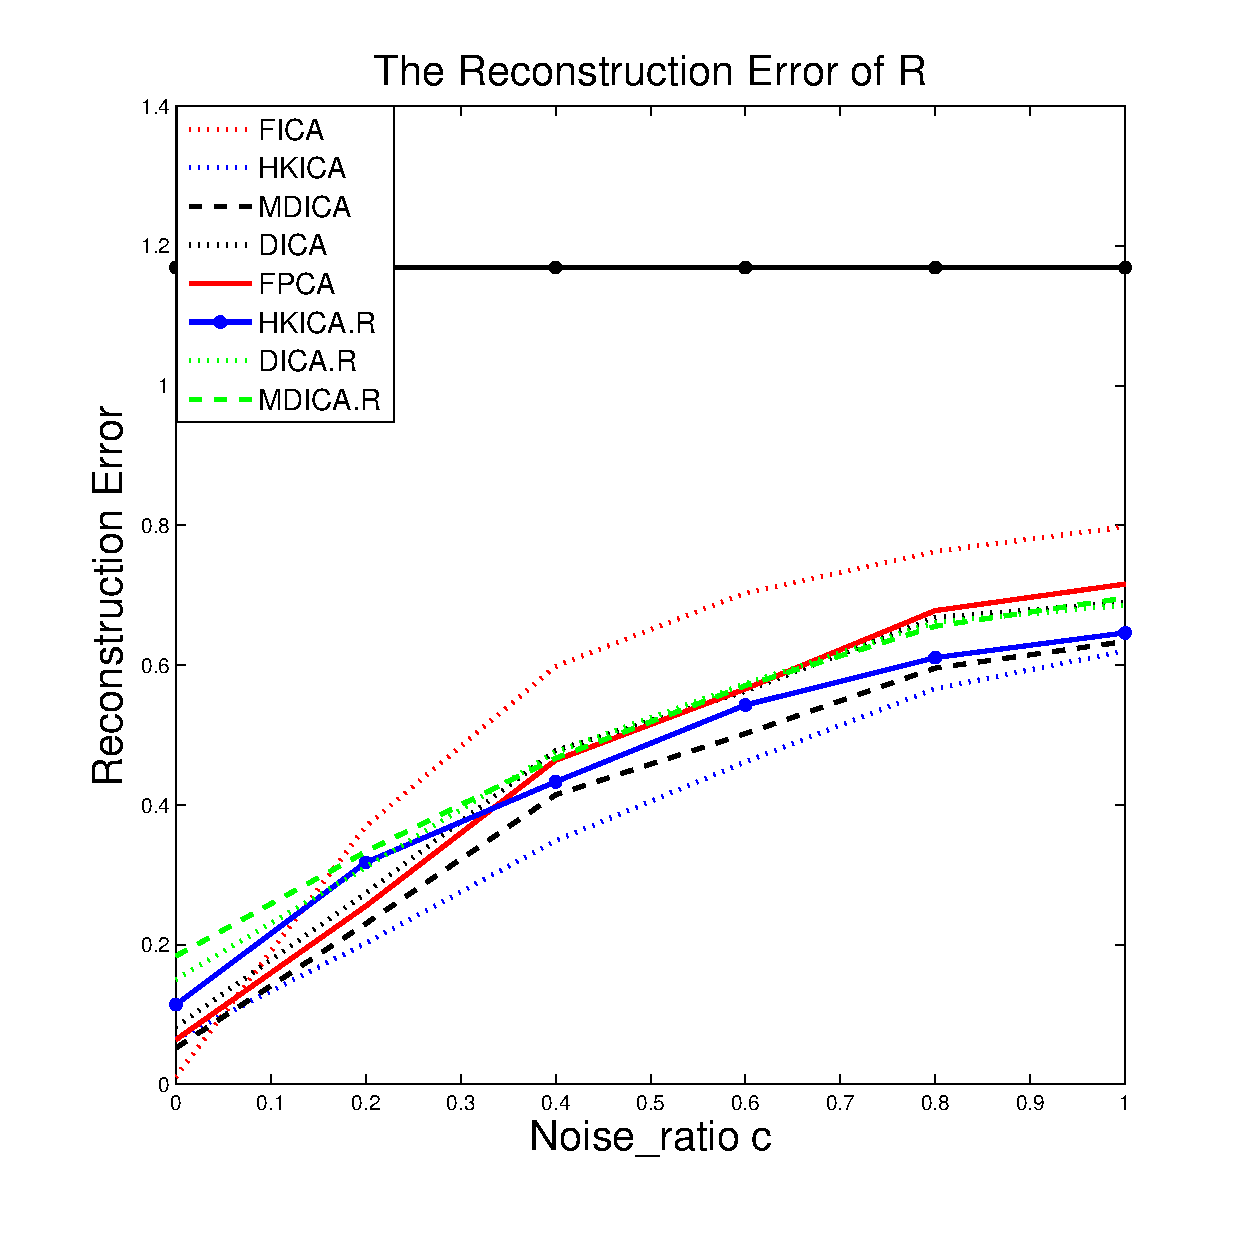
\includegraphics[width =0.45\columnwidth]{images/errorR_d3}
	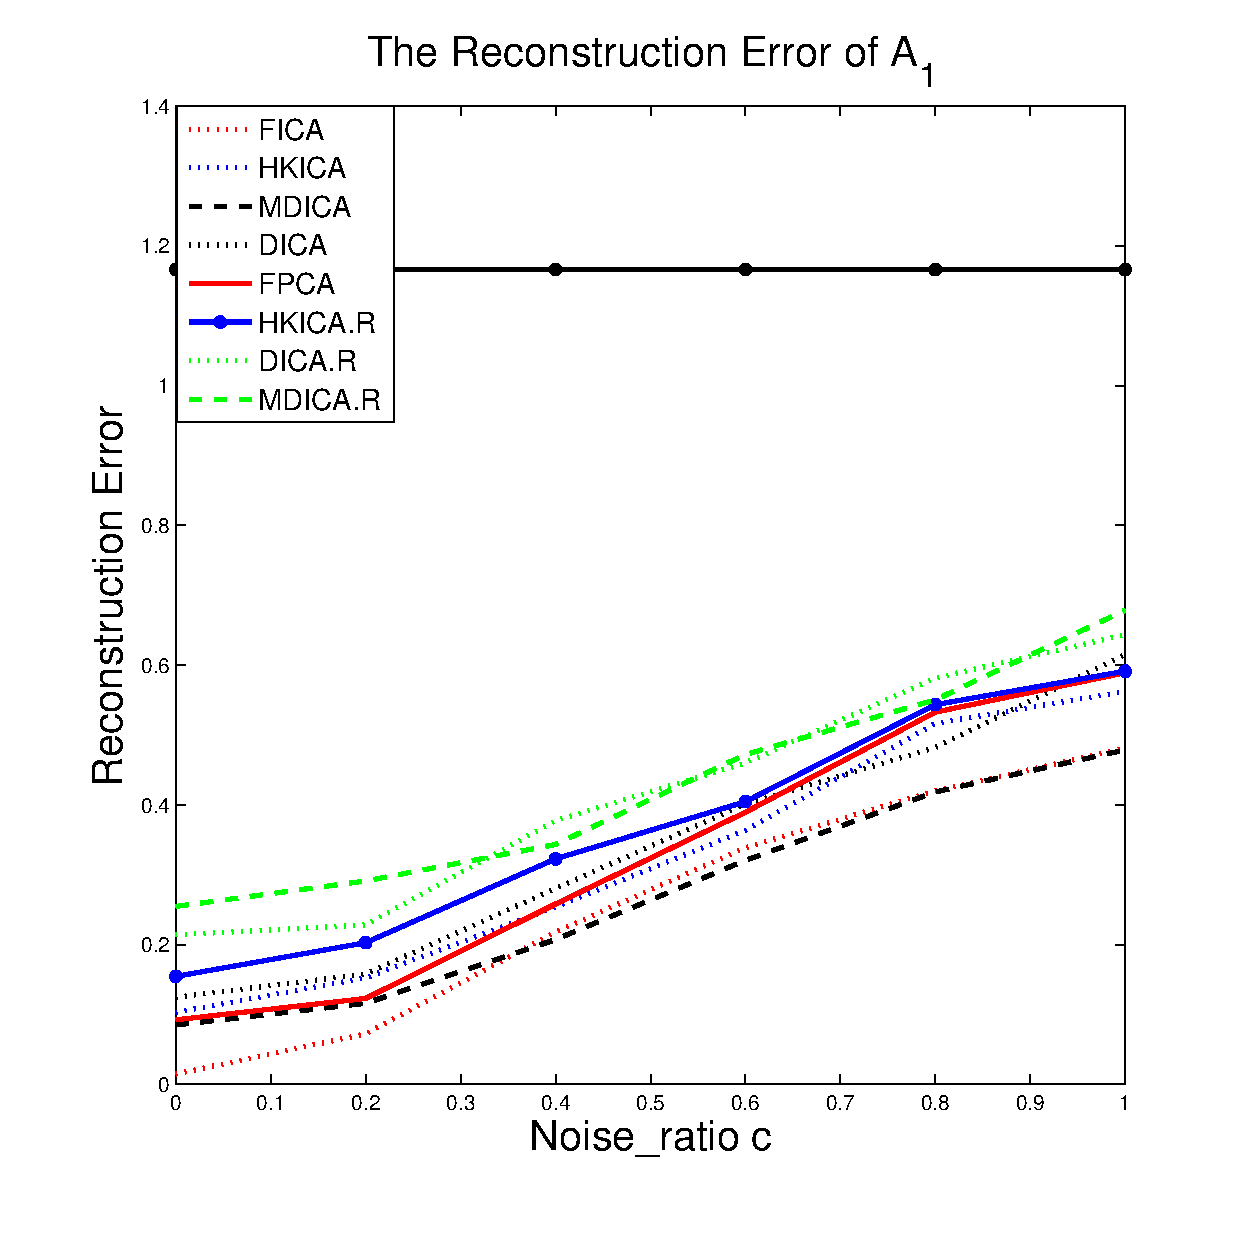
\includegraphics[width =0.45\columnwidth]{images/error1_d3} \\
	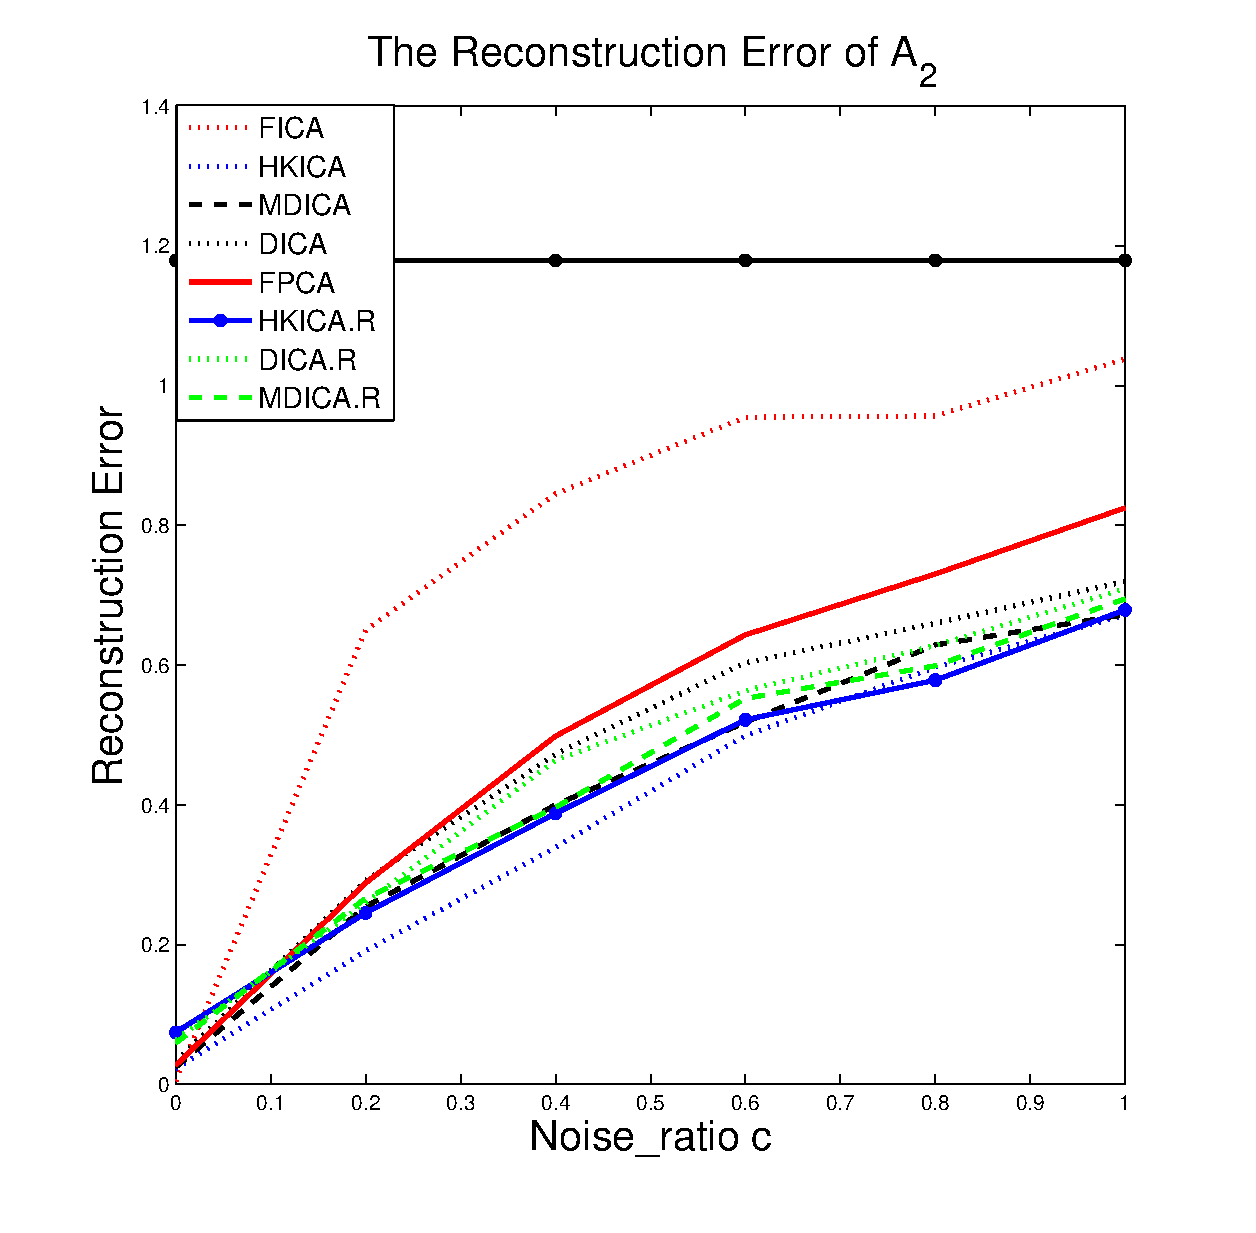
\includegraphics[width =0.45\columnwidth]{images/error2_d3}
	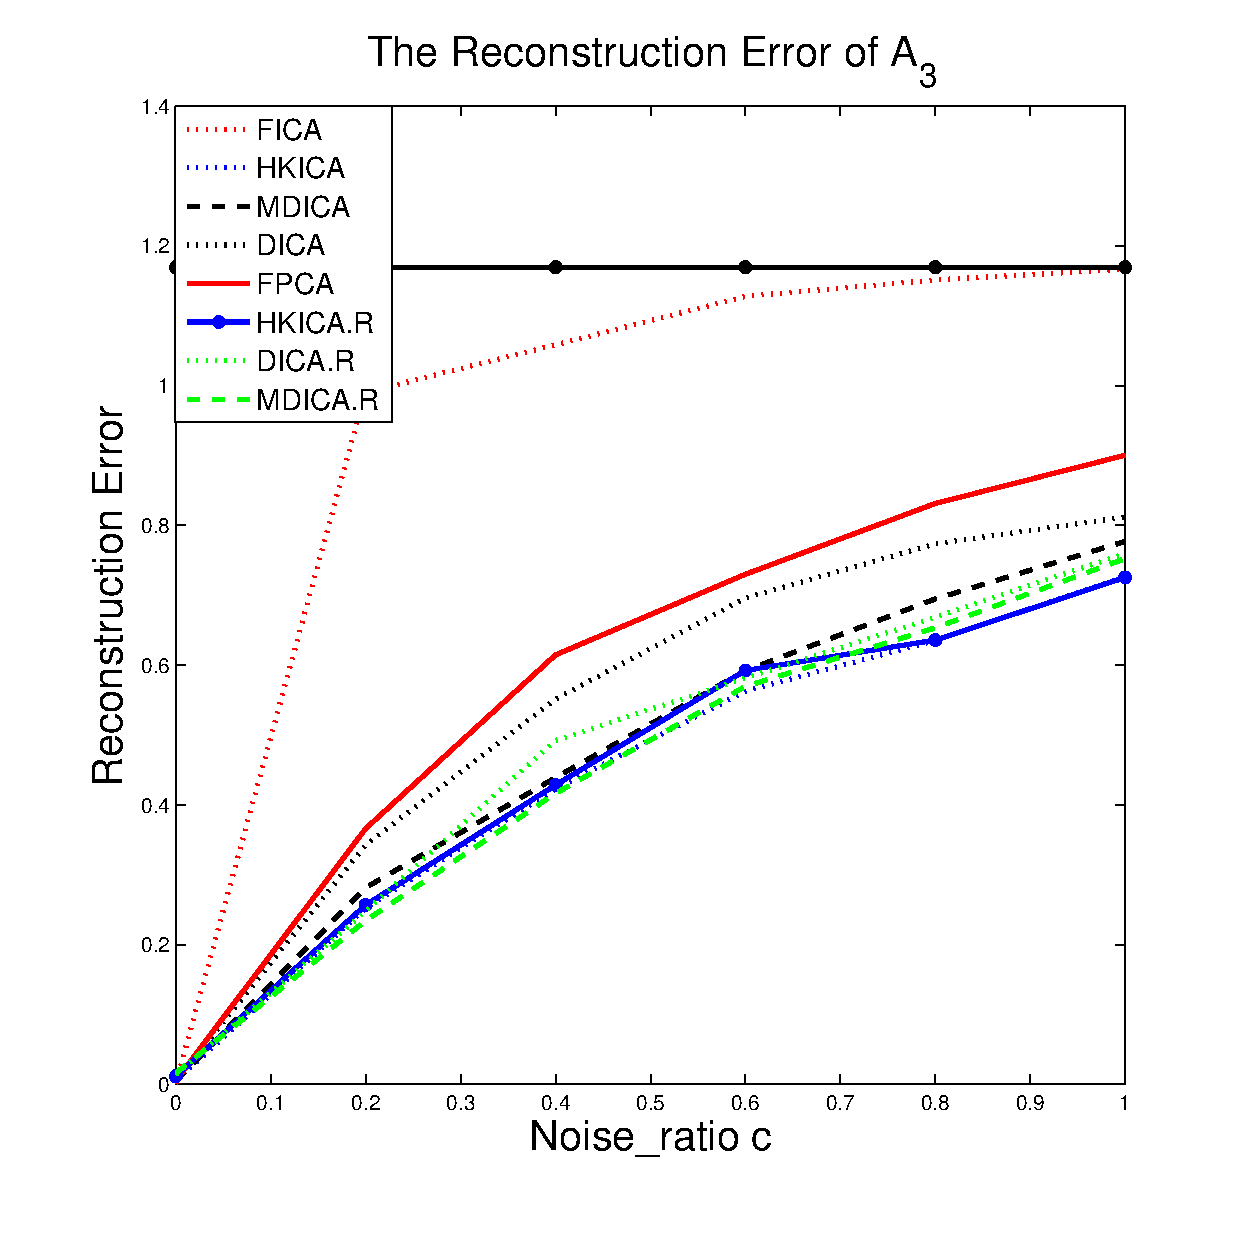
\includegraphics[width =0.45\columnwidth]{images/error3_d3}  \\
	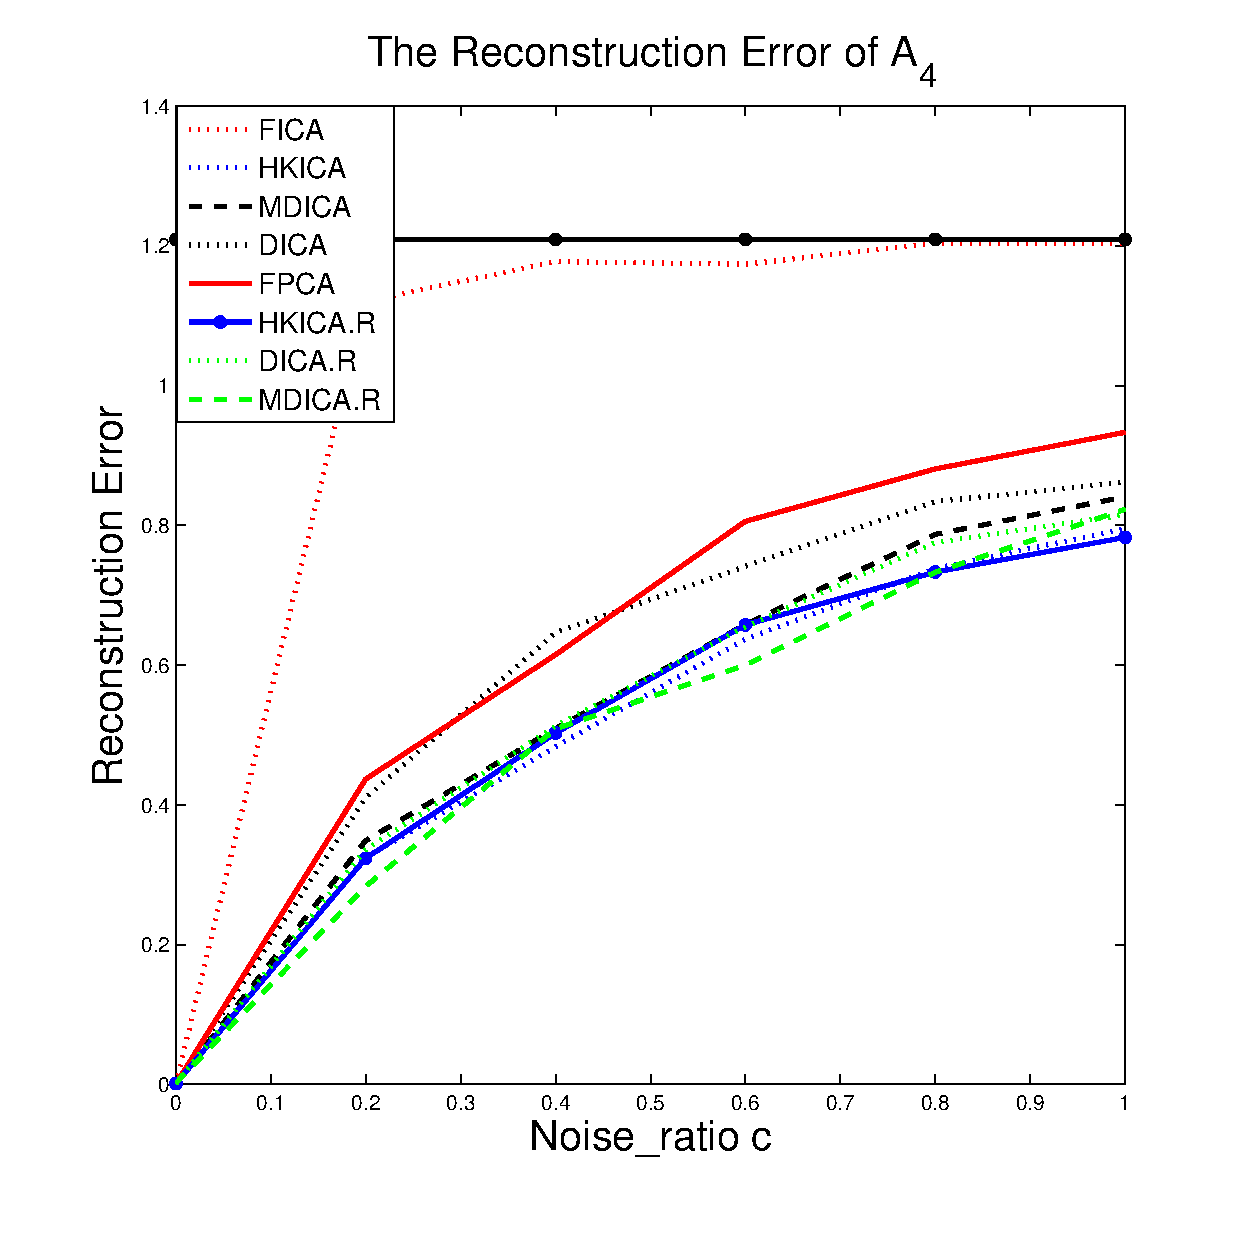
\includegraphics[width =0.45\columnwidth]{images/error4_d3}
\caption{
\label{fig:Error_d3}
 Reconstruction Errors: Dimension 3; X axis: noise ratio; Sample size: 20000.}
\end{figure}

\section{Experimental Results of different sample sizes}
\subsection{noise-free case}
The reconstruction errors for different sample sizes in a noise-free setting are as follows. 
\begin{figure}[t] %pt]
	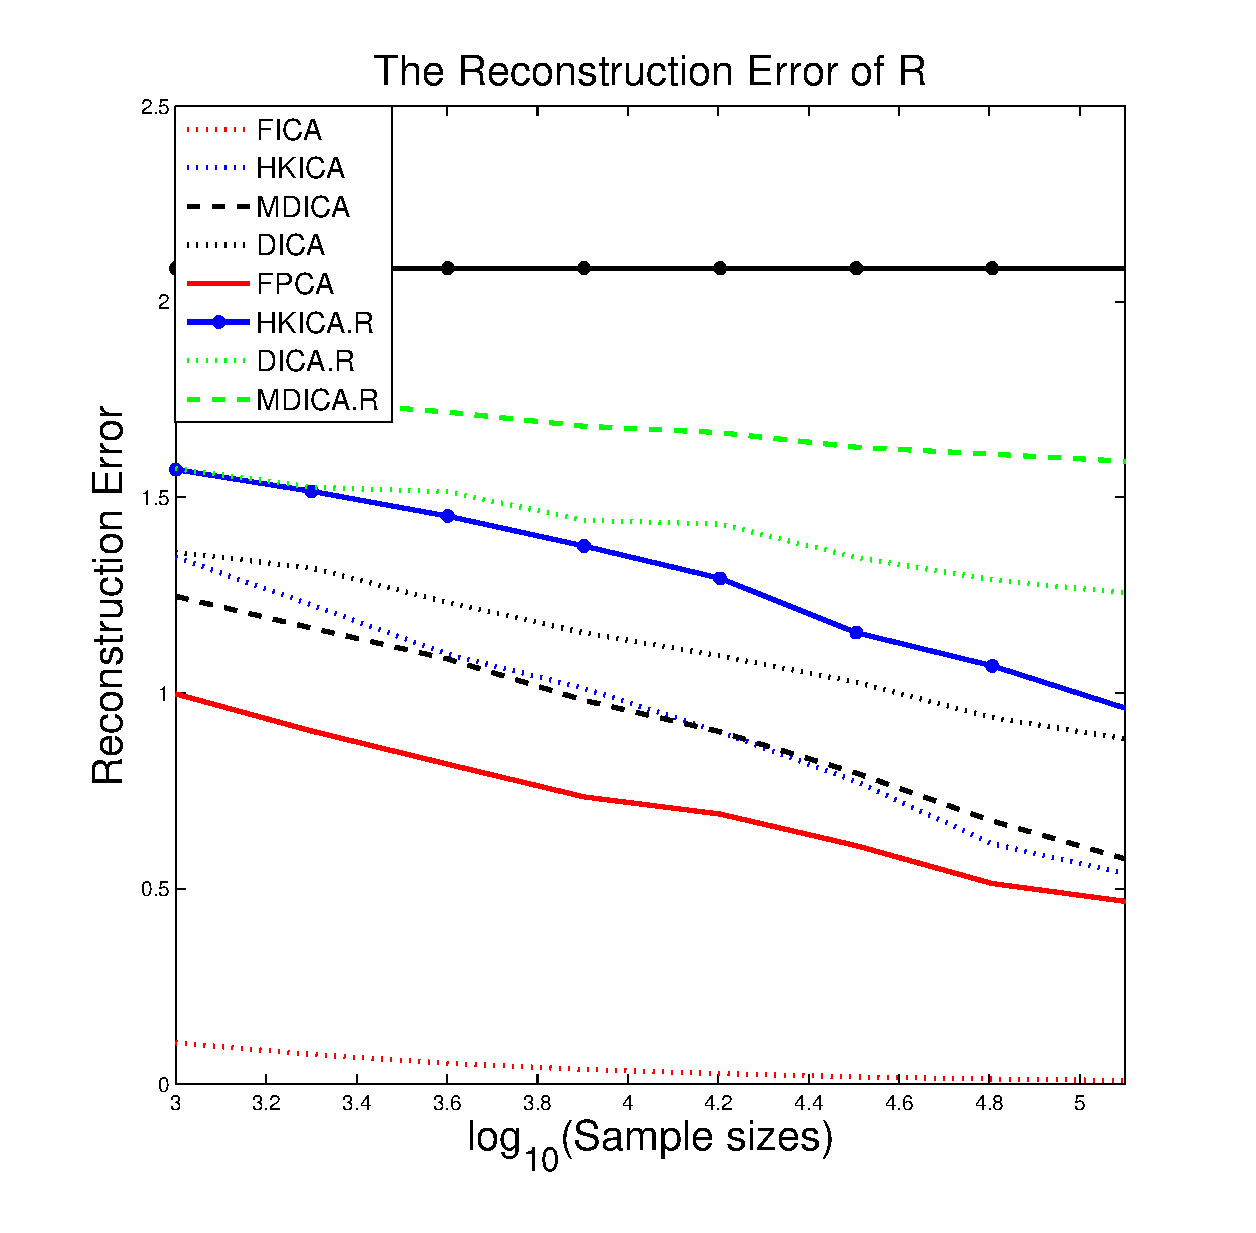
\includegraphics[width =0.45\columnwidth]{images/errorR_sample_noise0}
	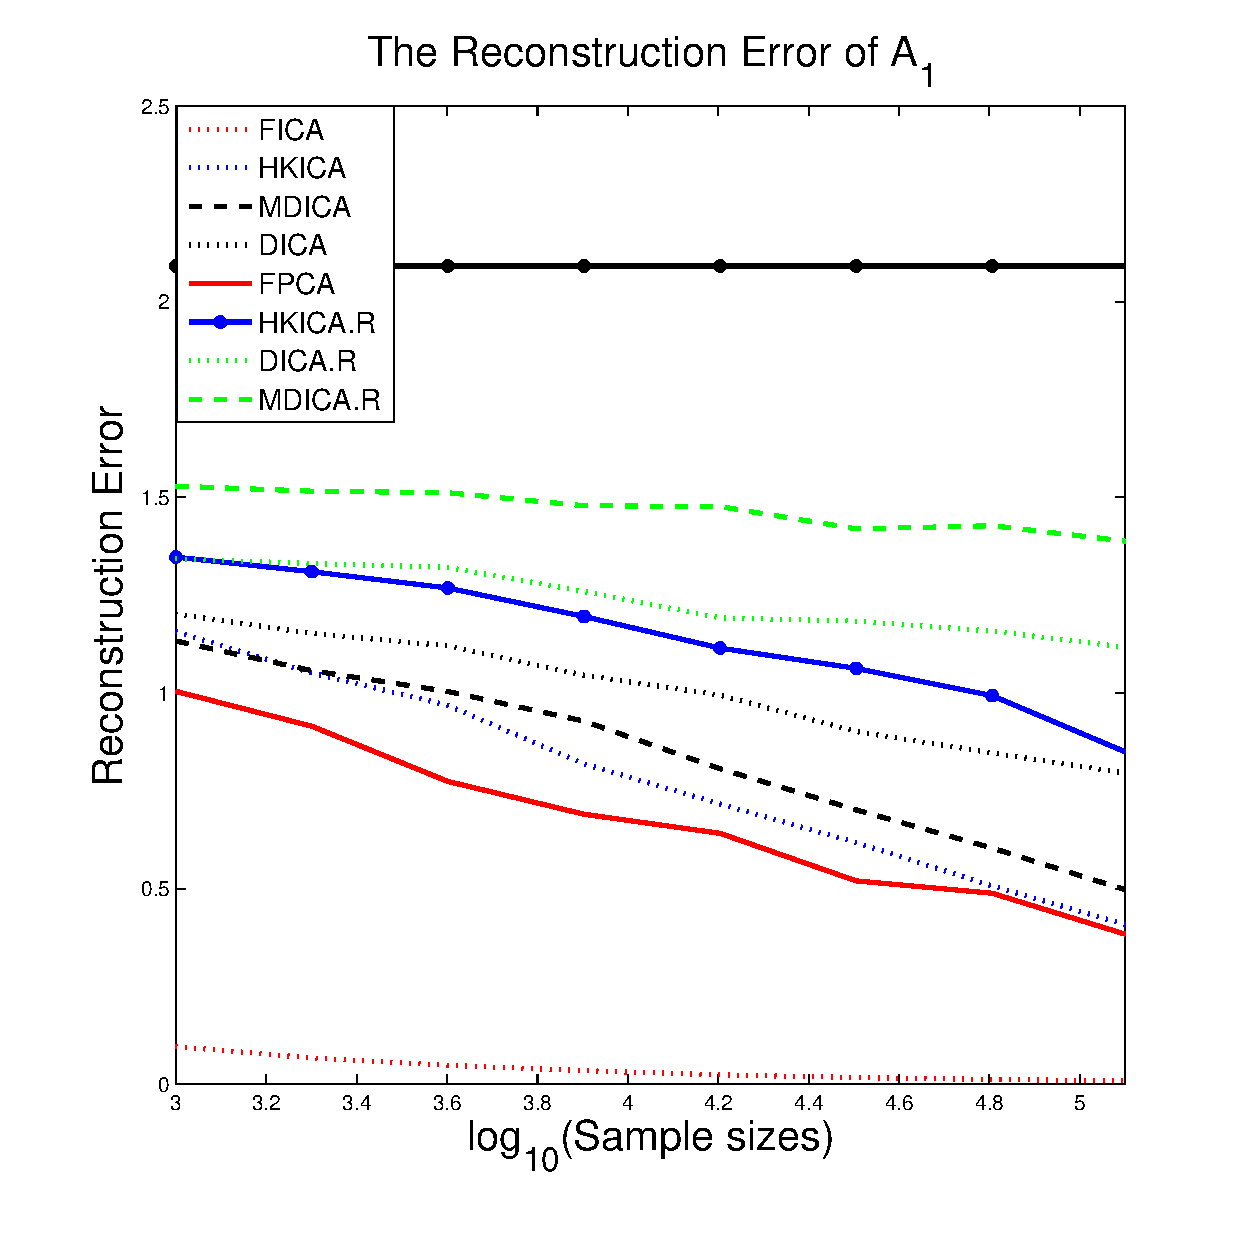
\includegraphics[width =0.45\columnwidth]{images/error1_sample_noise0} \\
	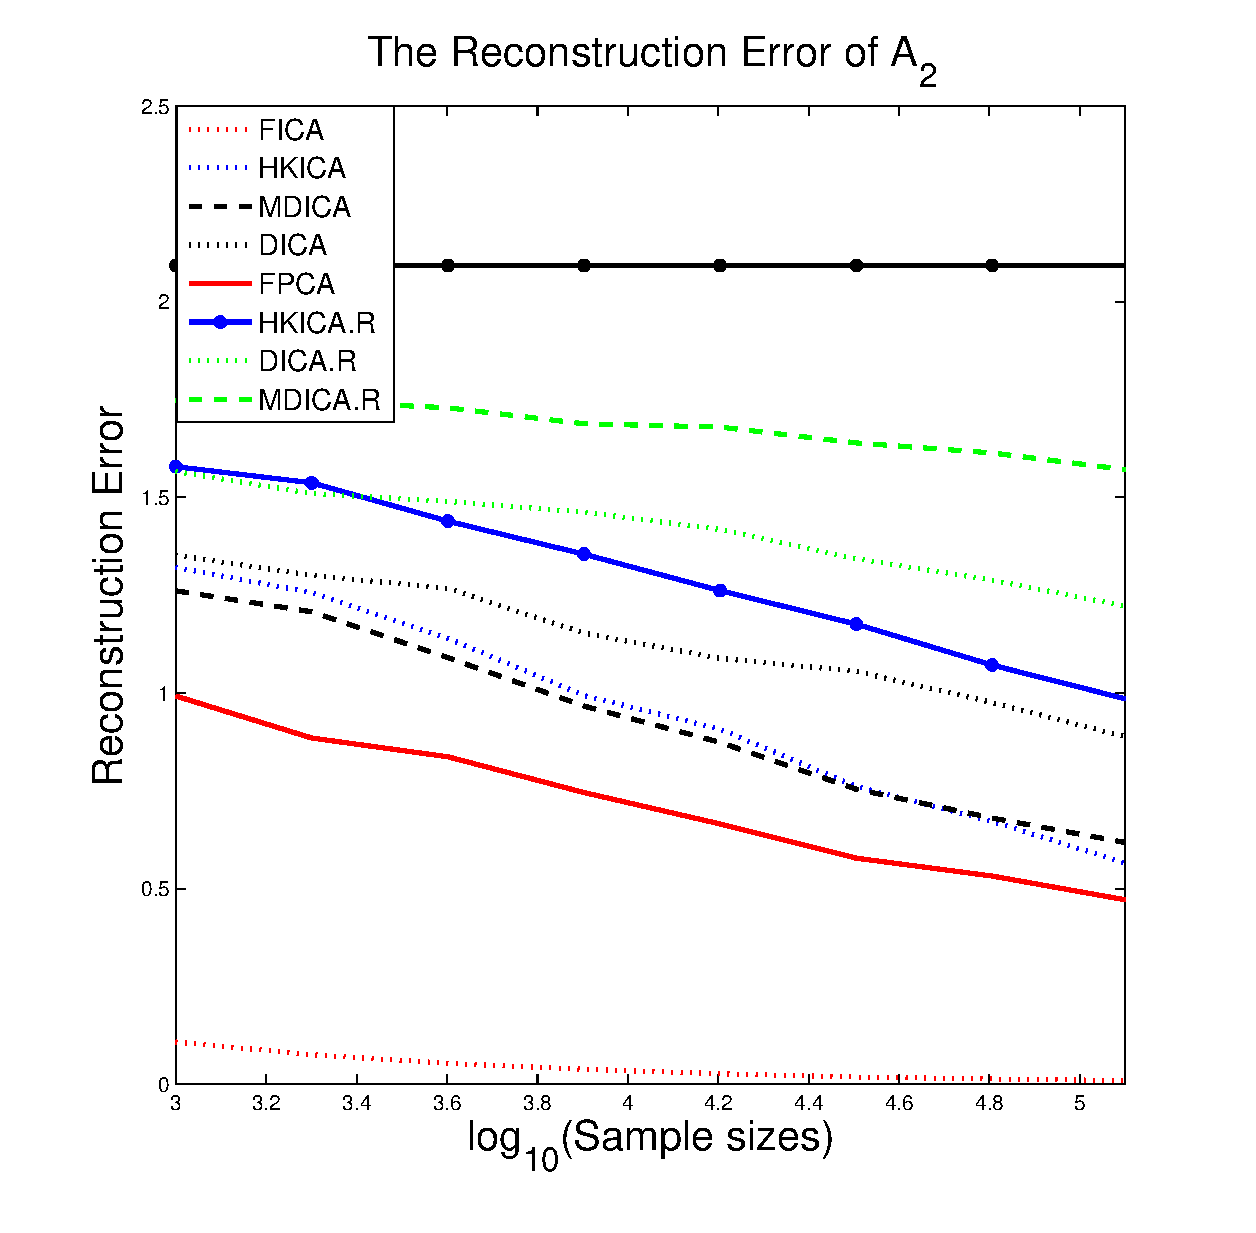
\includegraphics[width =0.45\columnwidth]{images/error2_sample_noise0}
	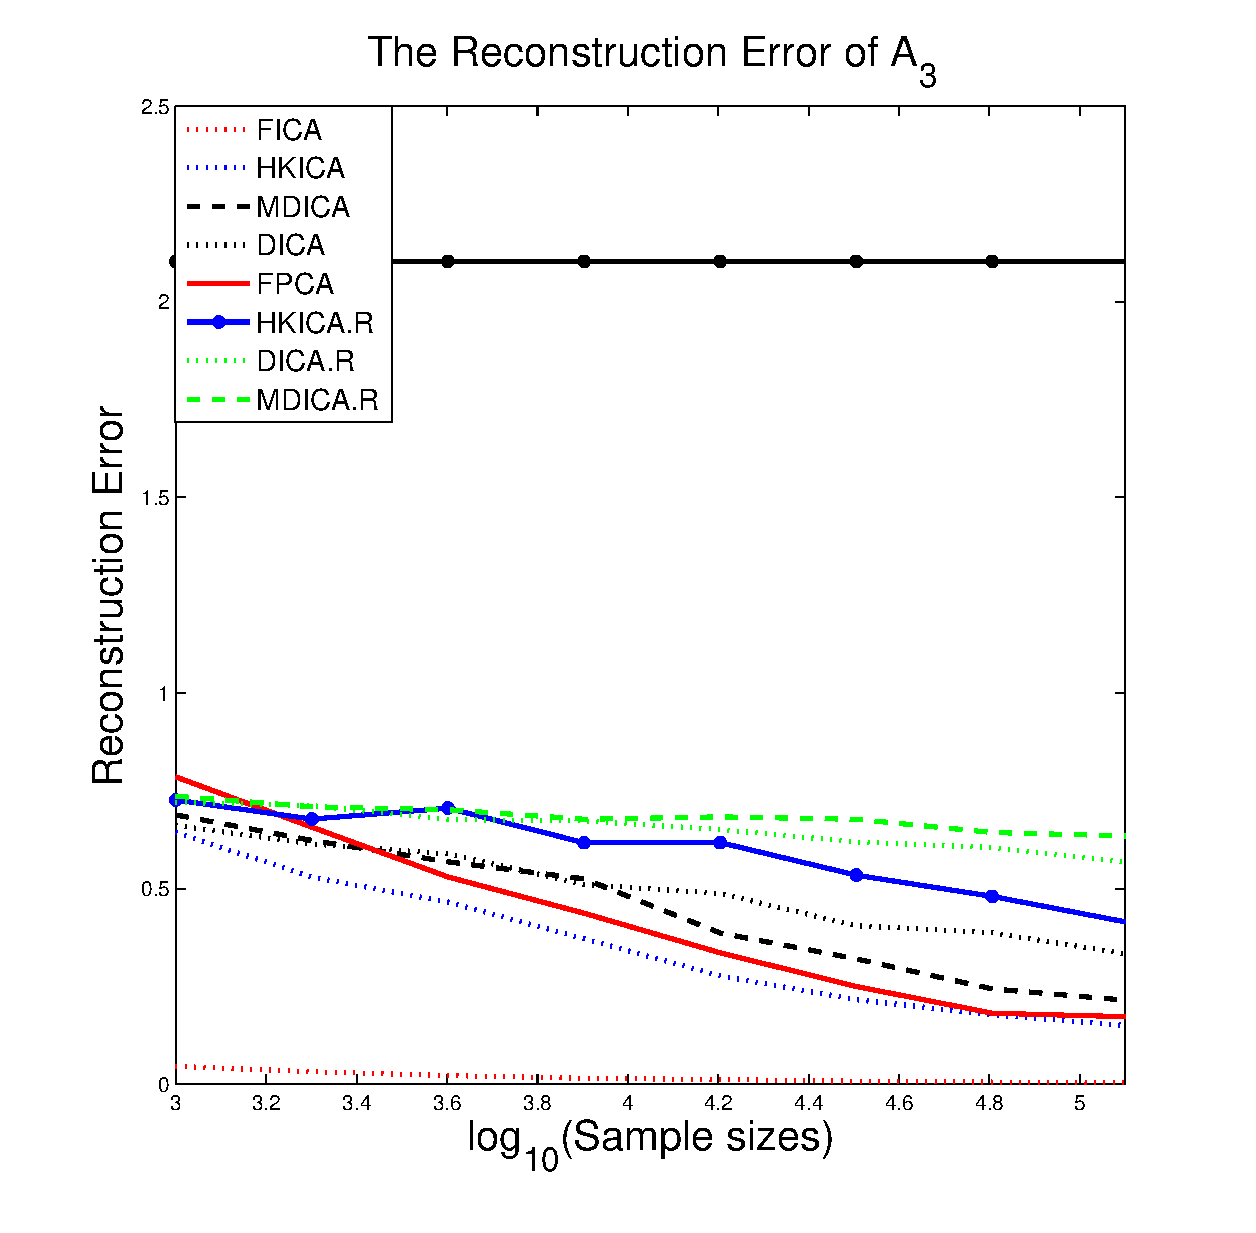
\includegraphics[width =0.45\columnwidth]{images/error3_sample_noise0} \\
	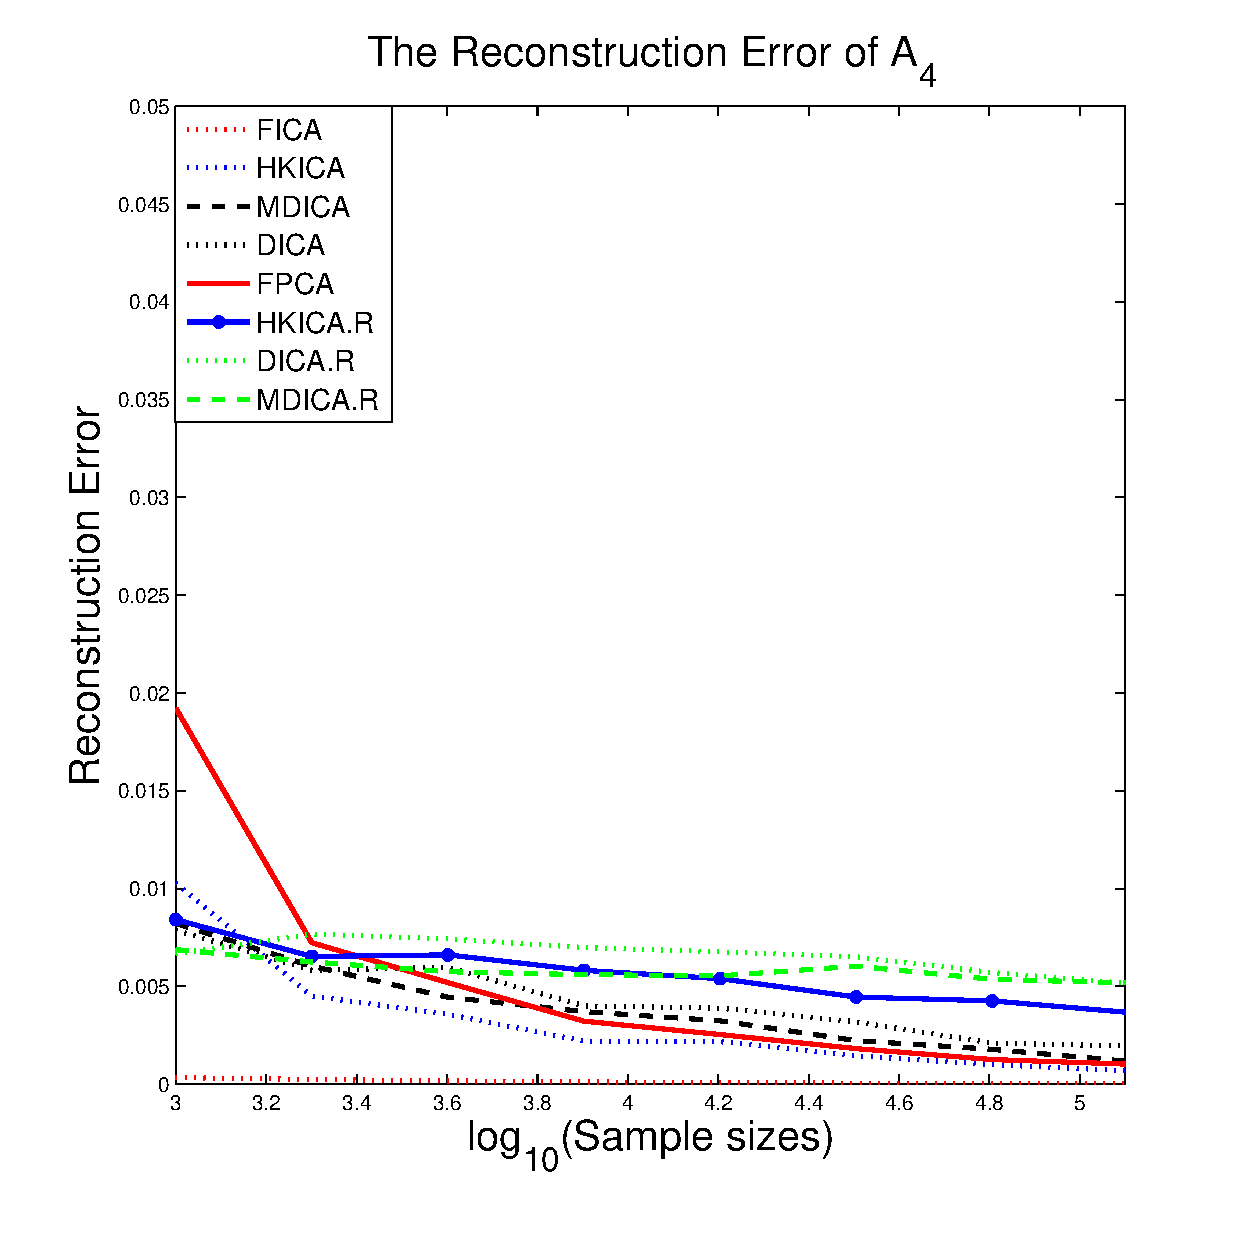
\includegraphics[width =0.45\columnwidth]{images/error4_sample_noise0}
\caption{
\label{fig:Error_sample_noise0}
 Reconstruction Errors: Dimension 6; X axis: sample size; Noise ratio: 0.}
\end{figure}

\subsection{the case of noise ratio 0.3}
The reconstruction errors for different sample sizes in a noise-free setting are as follows. 
\begin{figure}[t] %pt]
	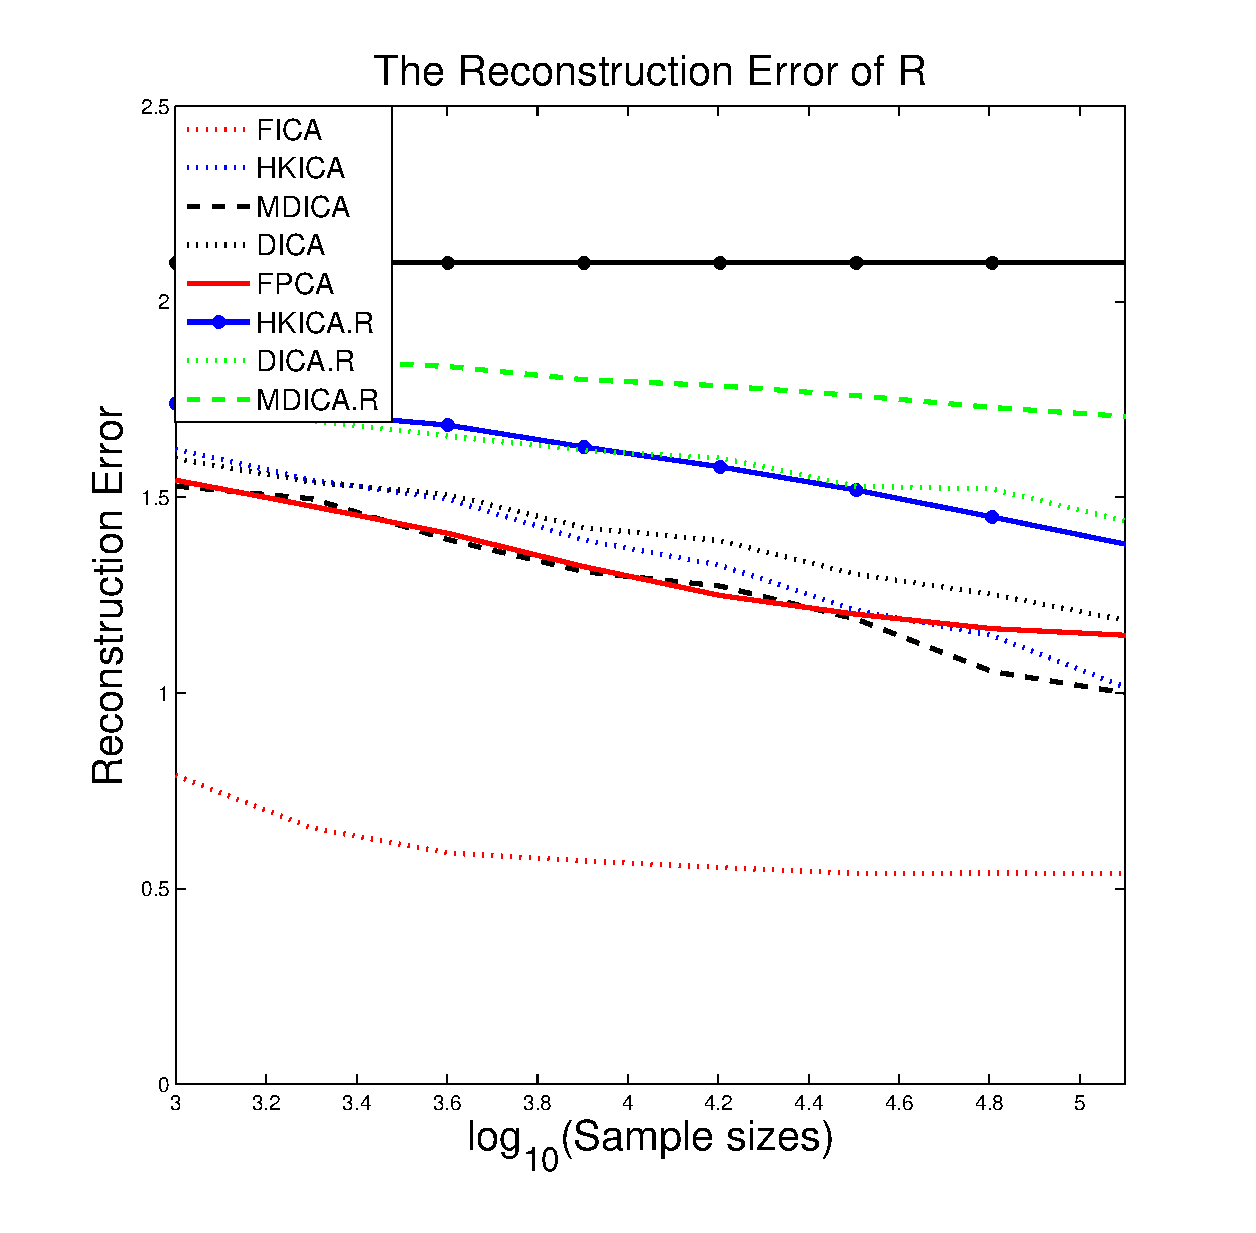
\includegraphics[width =0.45\columnwidth]{images/errorR_sample_noise3}
	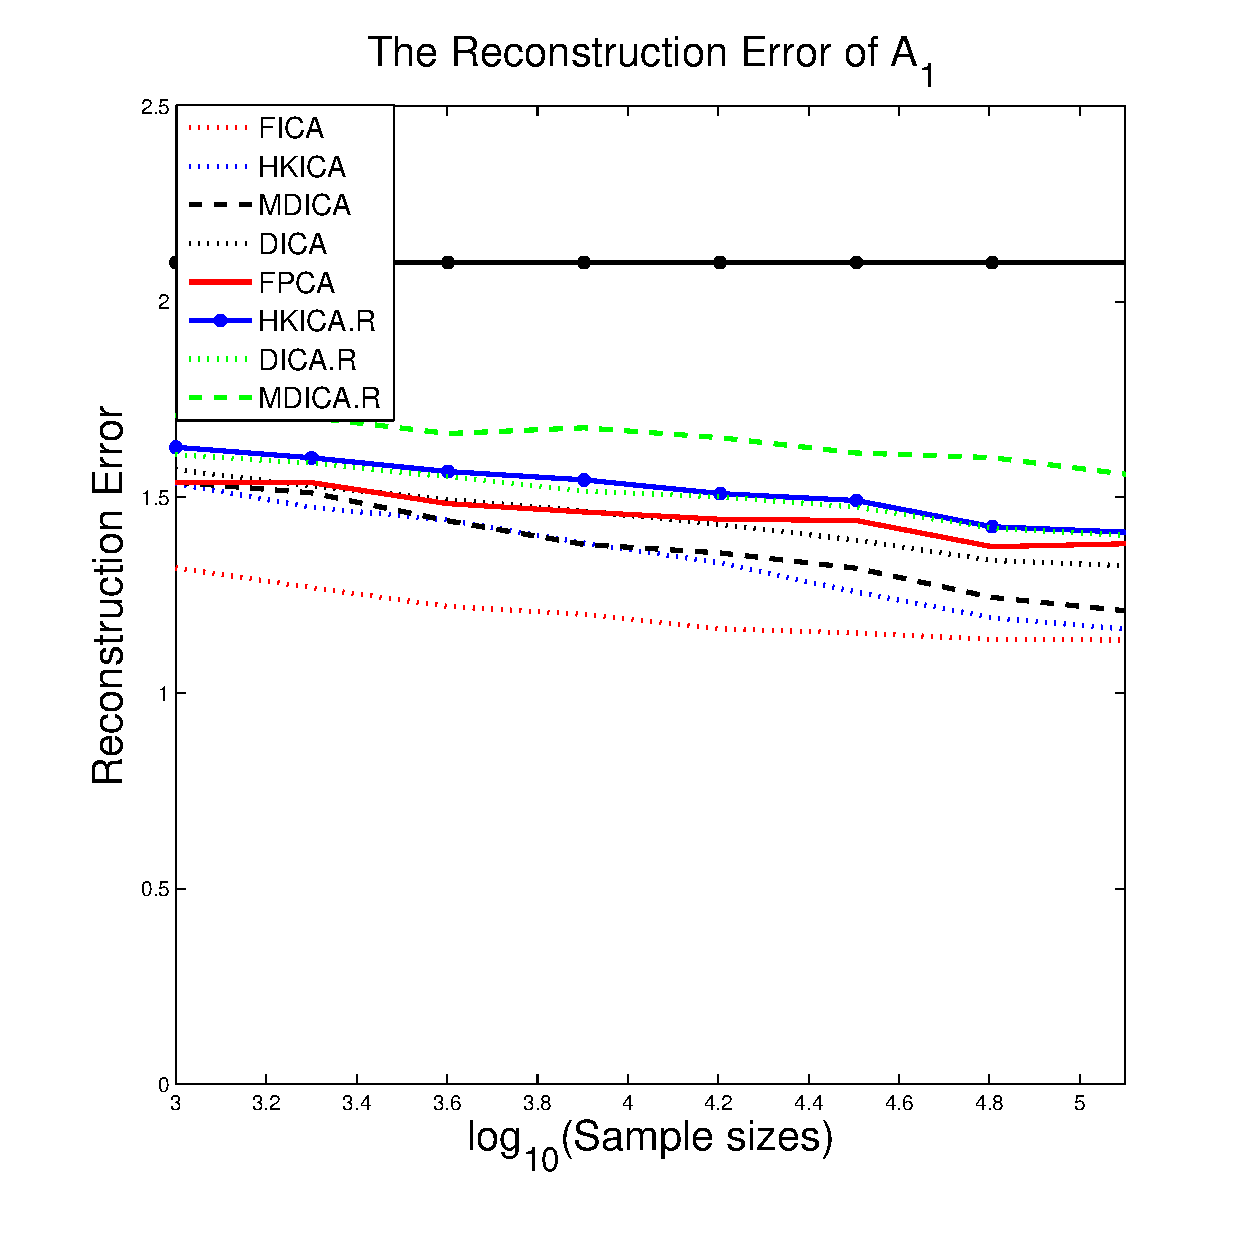
\includegraphics[width =0.45\columnwidth]{images/error1_sample_noise3} \\
	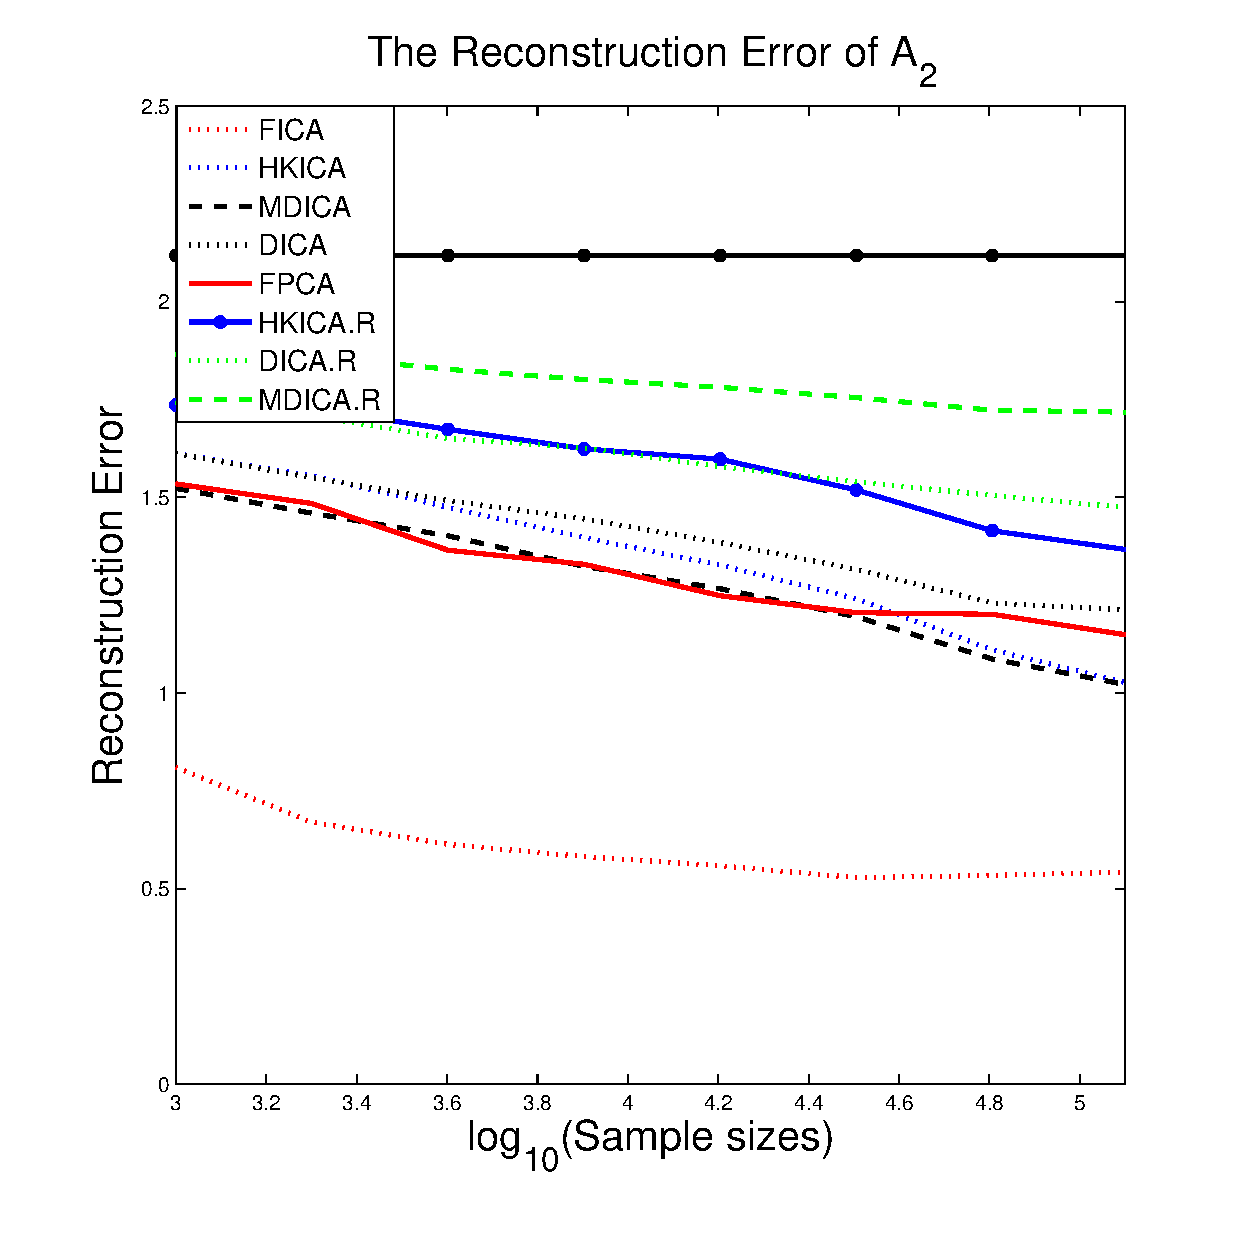
\includegraphics[width =0.45\columnwidth]{images/error2_sample_noise3}
	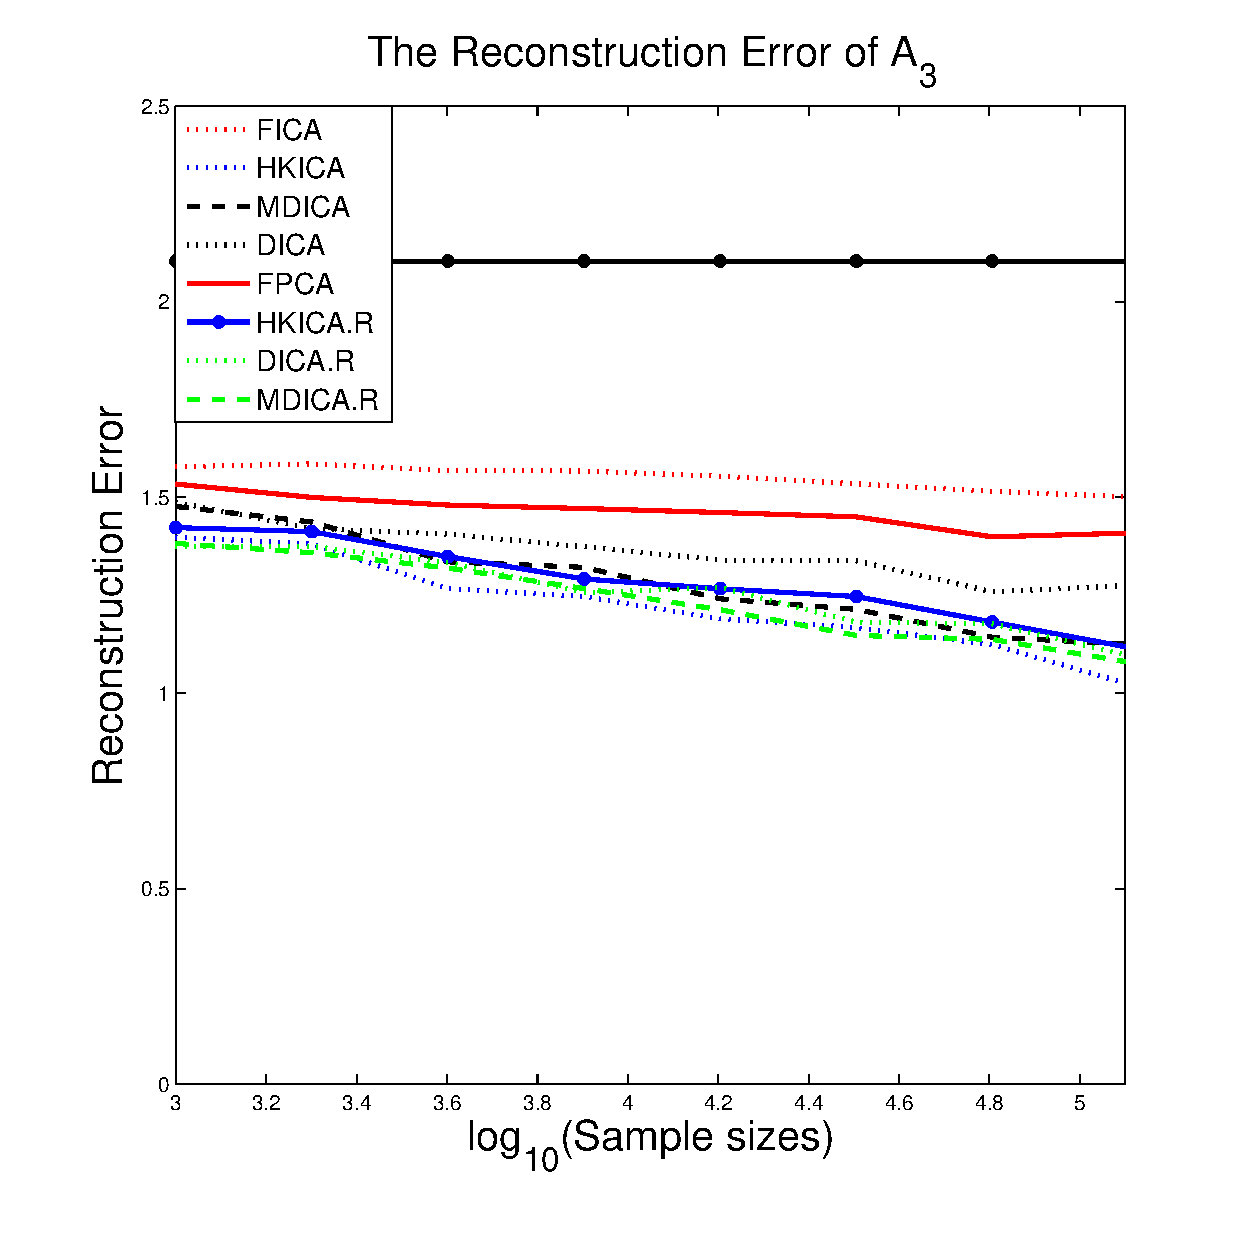
\includegraphics[width =0.45\columnwidth]{images/error3_sample_noise3} \\
	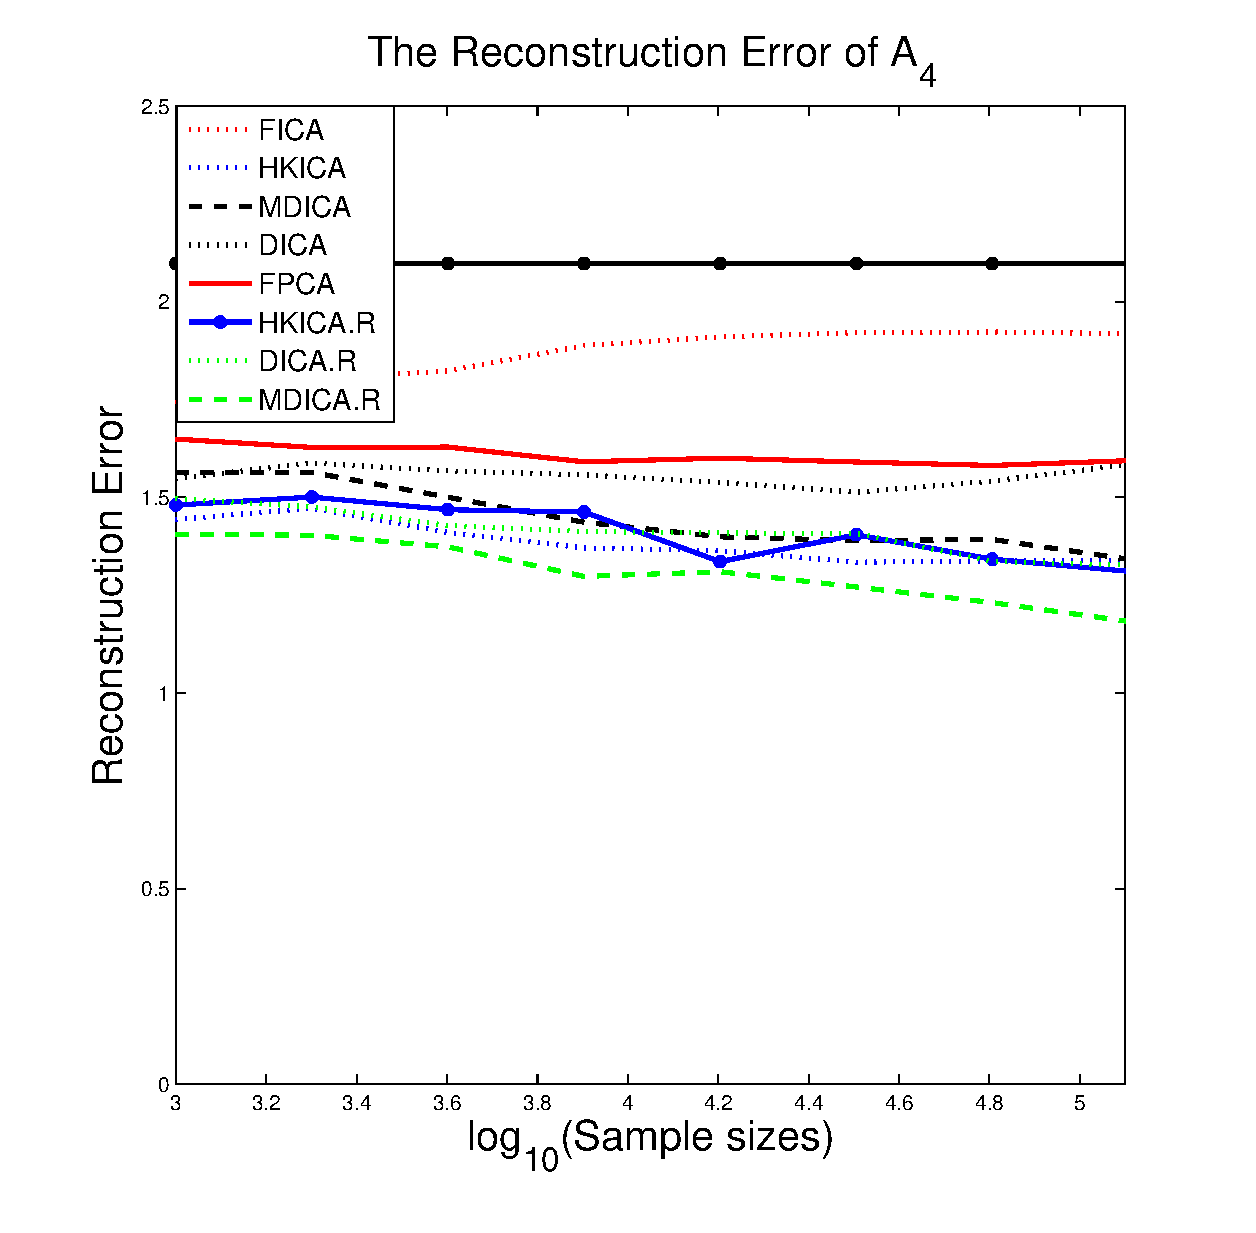
\includegraphics[width =0.45\columnwidth]{images/error4_sample_noise3}
\caption{
\label{fig:Error_sample_noise3}
 Reconstruction Errors: Dimension 6; X axis: sample size; Noise ratio: 0.3.}
\end{figure}

\subsection{the case of noise ratio 0.3}
The reconstruction errors for different sample sizes in a noise-free setting are as follows. 
\begin{figure}[t] %pt]
	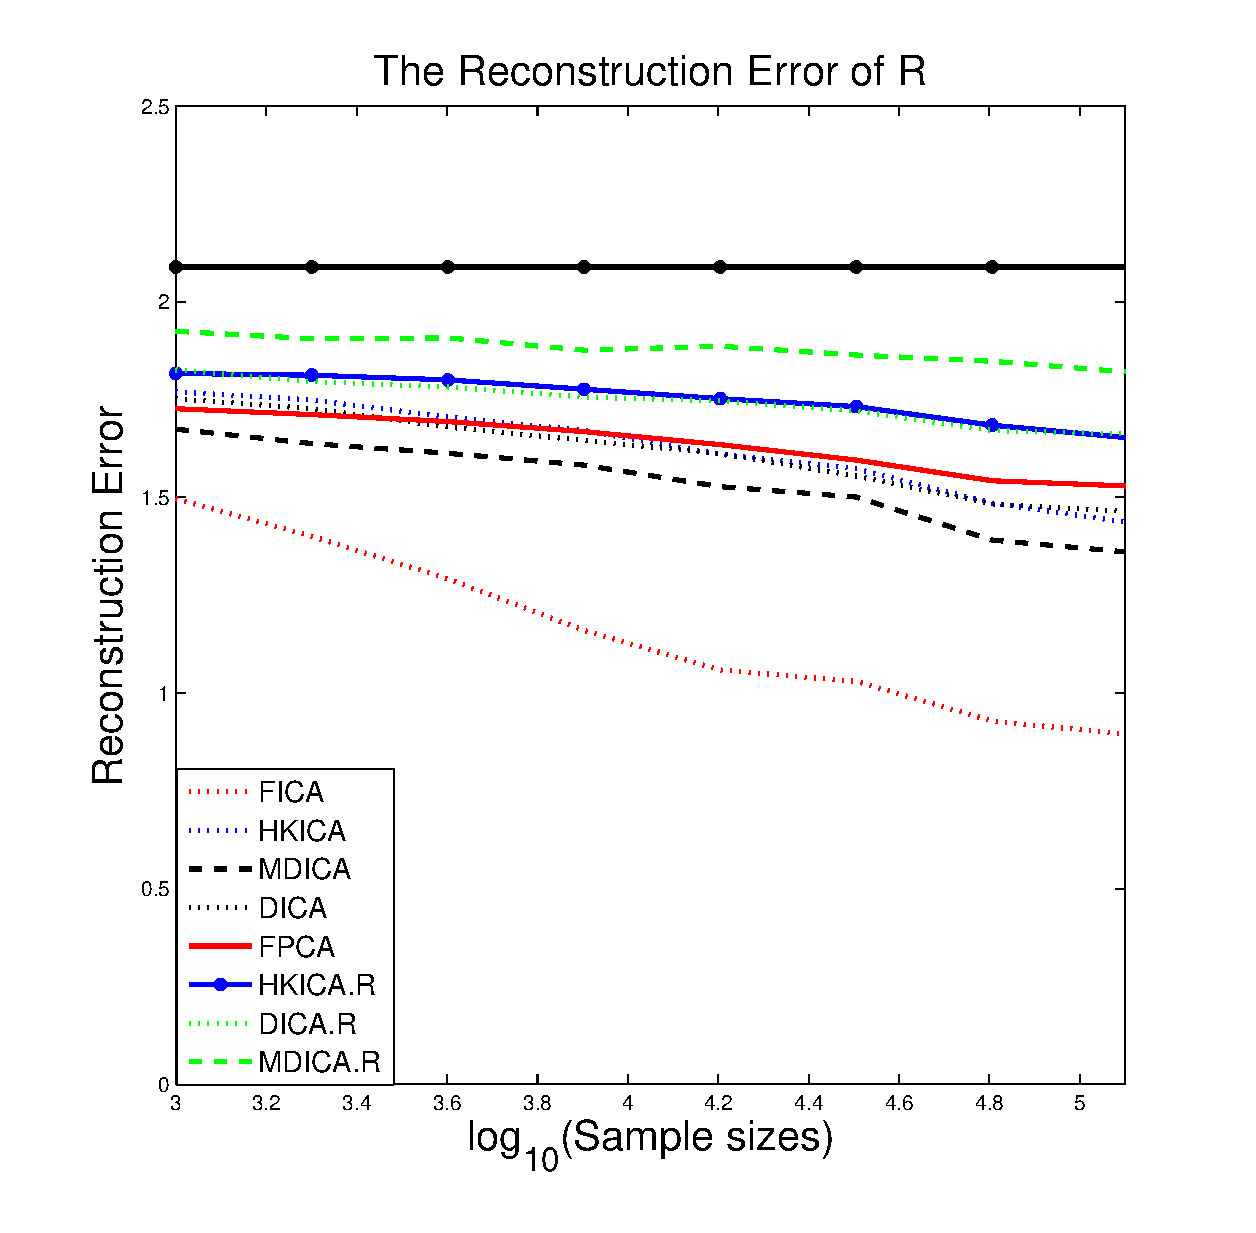
\includegraphics[width =0.45\columnwidth]{images/errorR_sample_noise6}
	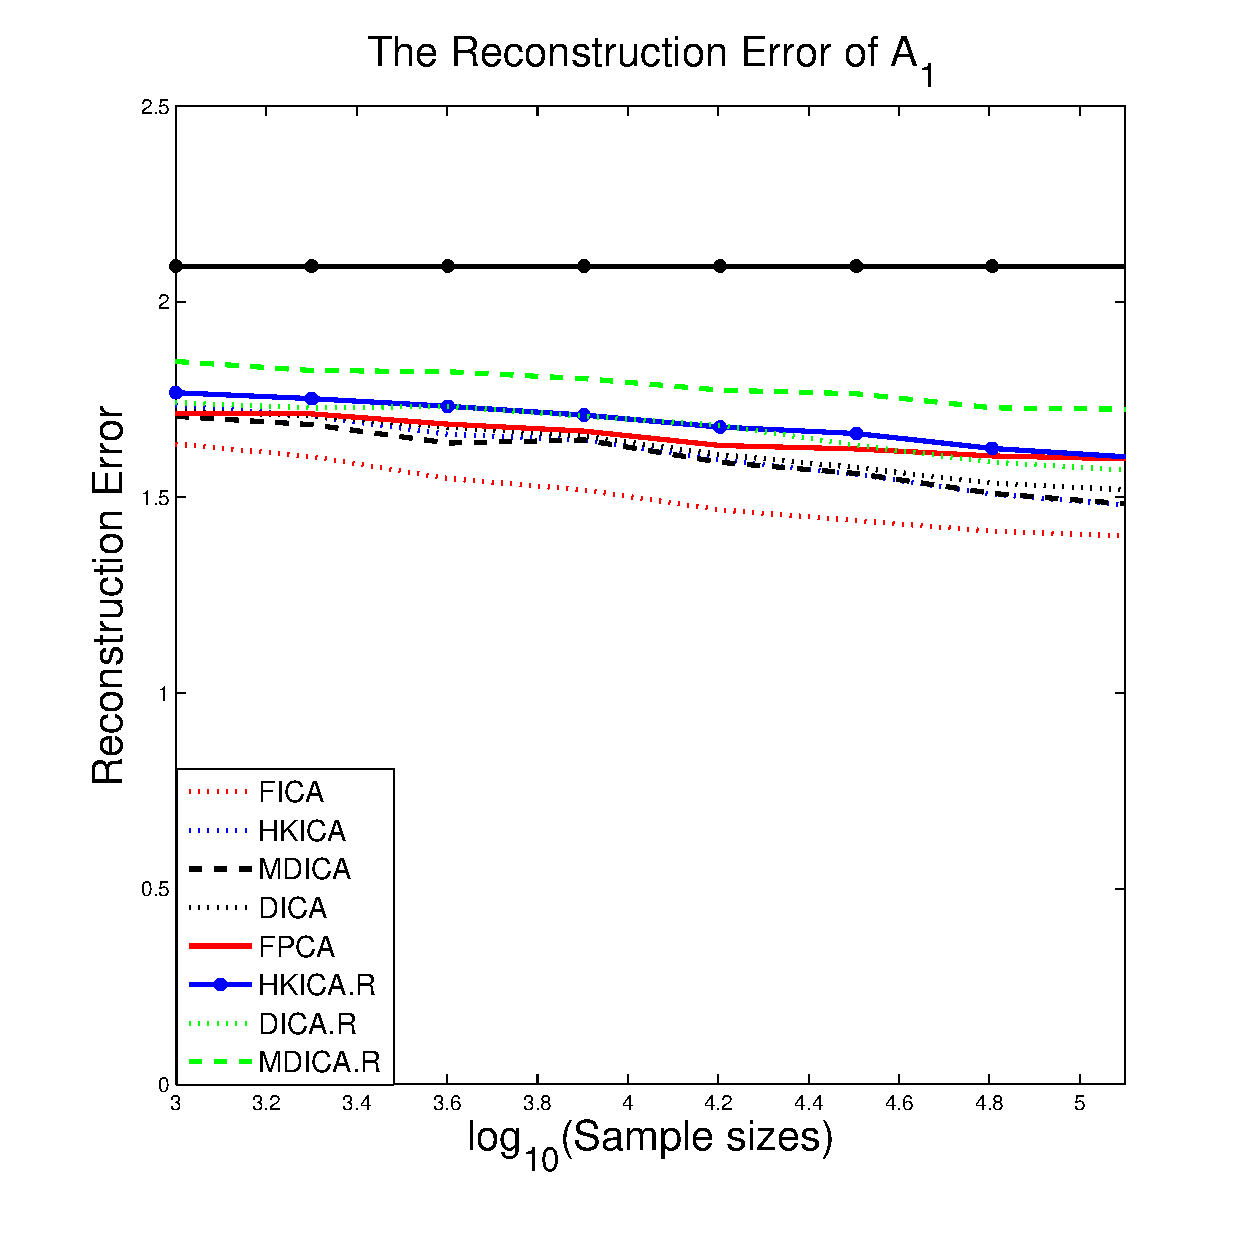
\includegraphics[width =0.45\columnwidth]{images/error1_sample_noise6} \\
	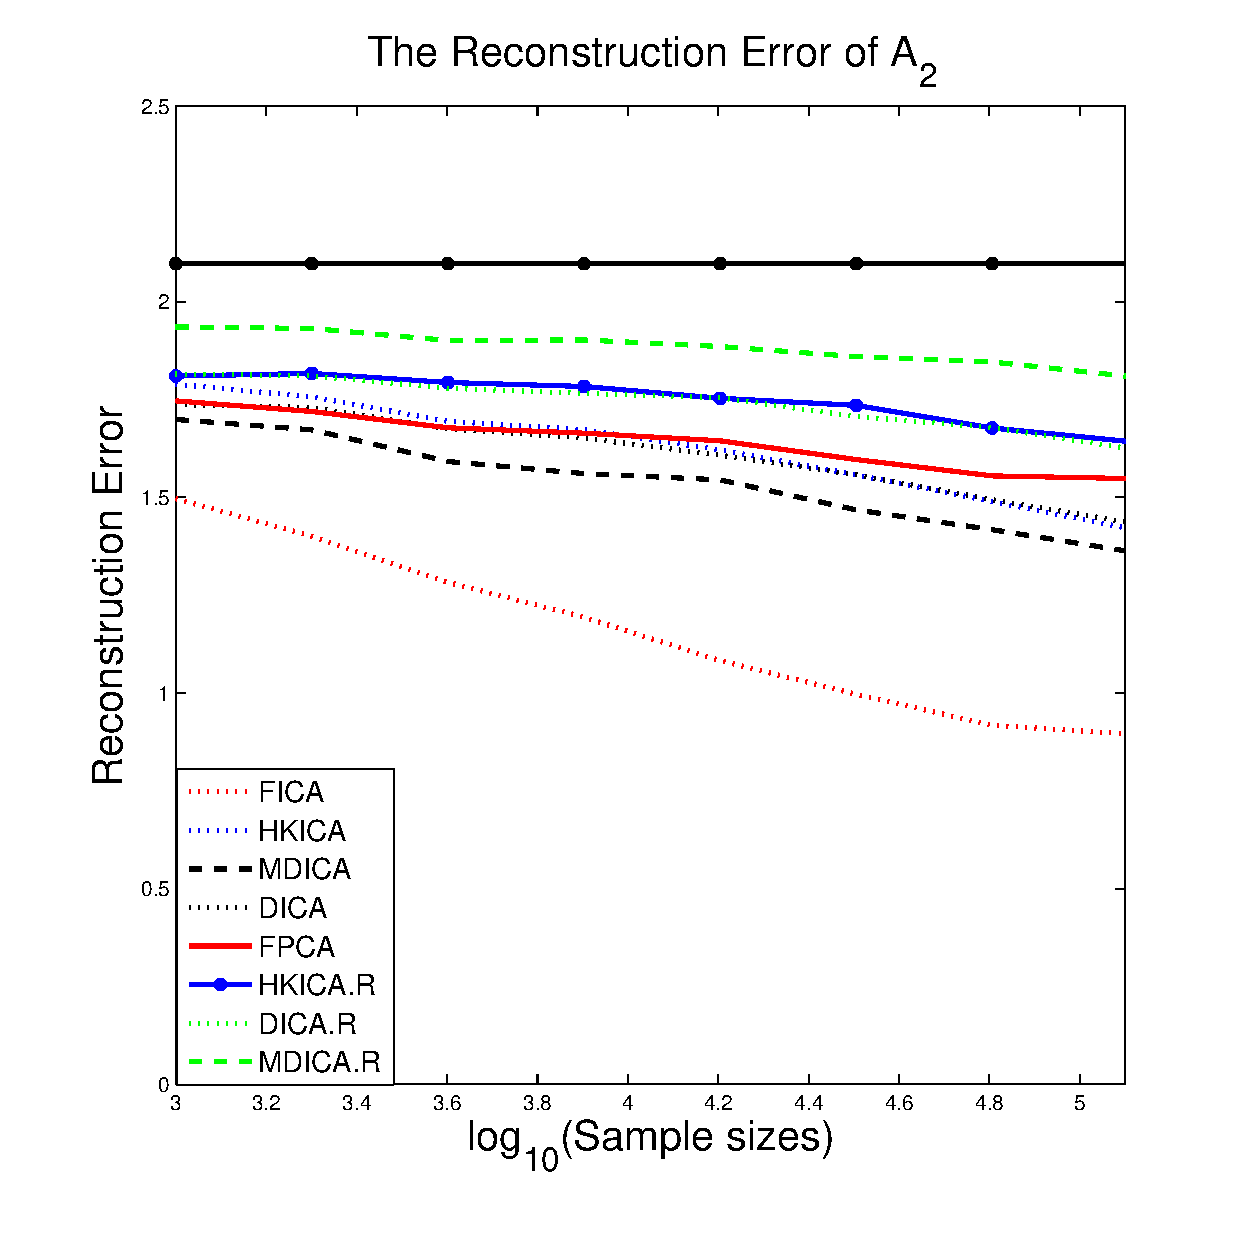
\includegraphics[width =0.45\columnwidth]{images/error2_sample_noise6}
	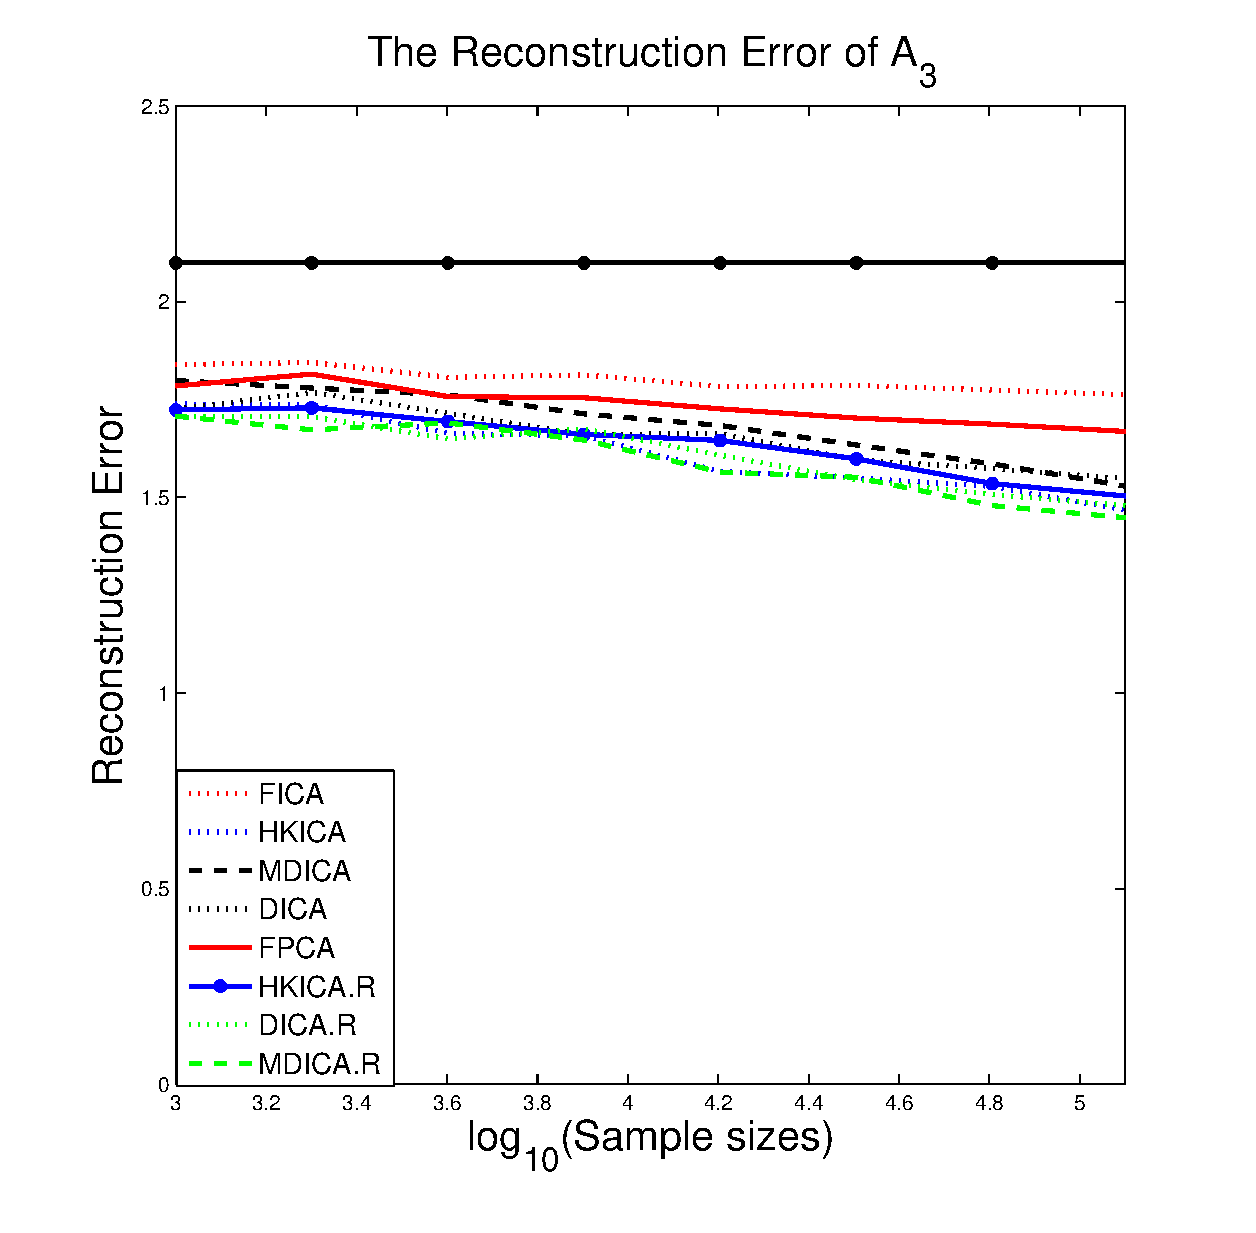
\includegraphics[width =0.45\columnwidth]{images/error3_sample_noise6} \\
	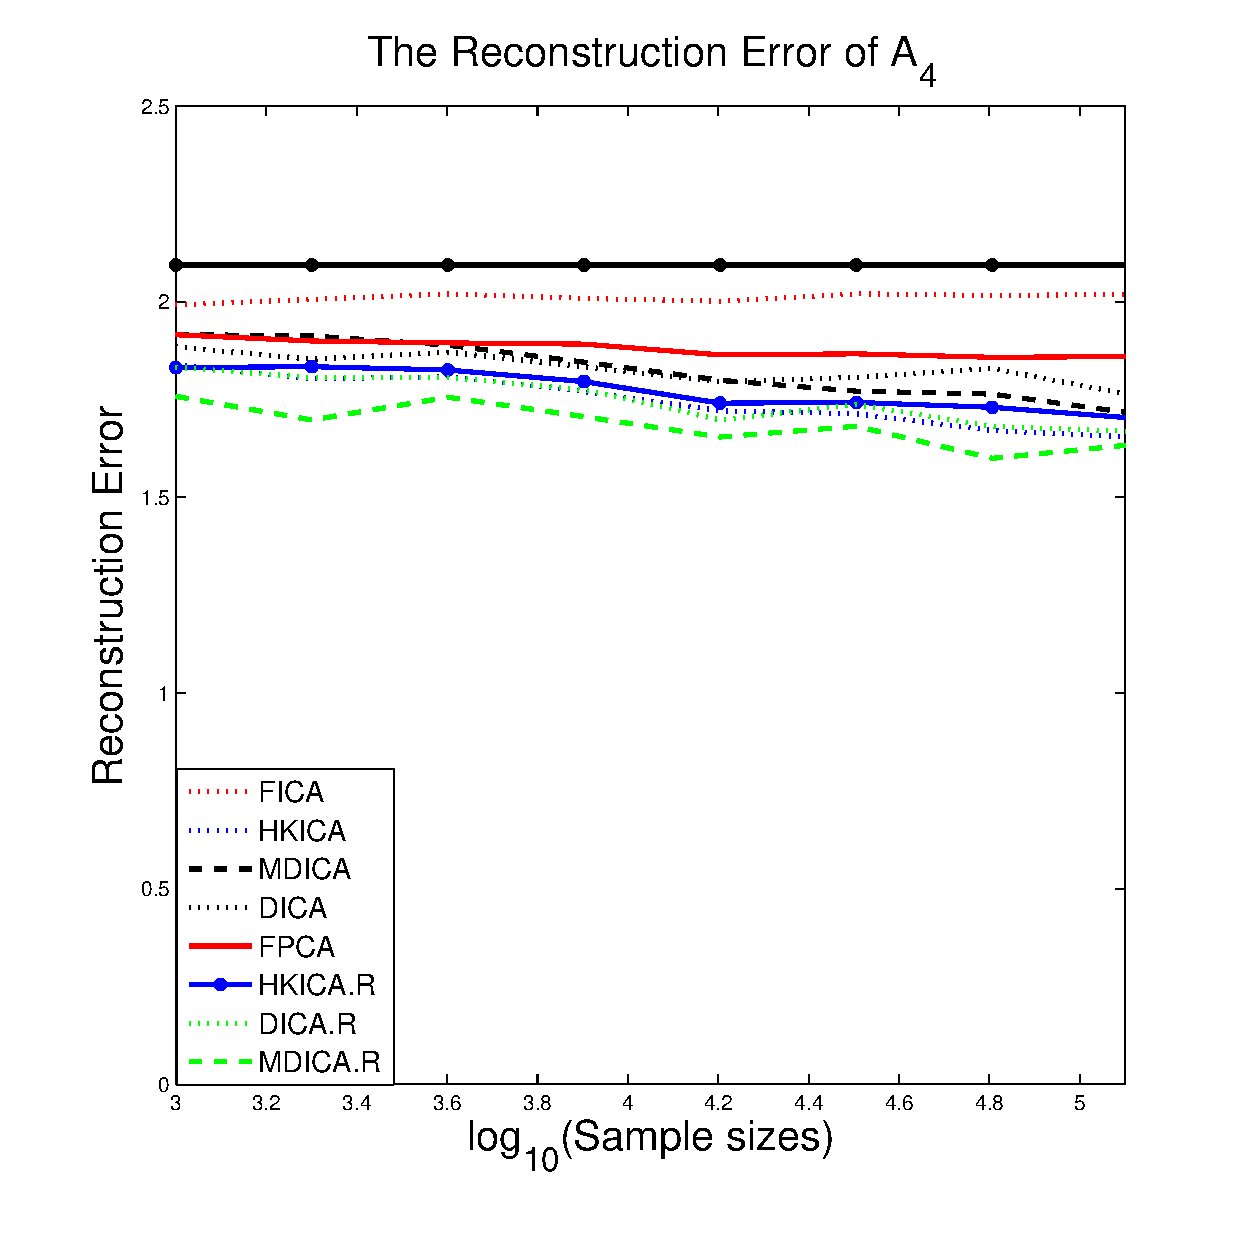
\includegraphics[width =0.45\columnwidth]{images/error4_sample_noise6}
\caption{
\label{fig:Error_sample_noise6}
 Reconstruction Errors: Dimension 6; X axis: sample size; Noise ratio: 0.6.}
\end{figure}
\fi

%%% Local Variables: 
%%% mode: latex
%%% TeX-master: "DICA"
%%% End: 
